 % The main file for CAMP reports
 % Don't put any content in here. 
 % Don't even include content files by using \input or \inlcude. 
 % Put your content to TEXT.TEX or include it there using \input.
 % Uses:
 %		SETTINGS.TEX	contains the settings for this document
 %		COMMANDS.TEX	contains commands which can be used while writing
 %		INFO.TEX			contains the author, title and so on for the cover
 %		COVER.TEX			formats the front cover of the document
 %		ABSTRACT.TEX	contains the abstract to be included (if needed)
 %		TEXT.TEX			contains the actual content of the document
 %		BIB.BIB				containt the BibTeX entries for the document
 
 
%% Draft document mode
%% Final document
\documentclass[11pt,a4paper,bibtotoc,idxtotoc,headsepline,footsepline,footexclude,BCOR12mm,DIV13]{scrbook}

%\documentclass[11pt,a4paper,bibtotoc,idxtotoc,headsepline,footsepline,footexclude,BCOR20mm,DIV10]{scrbook}

% KOMA-Optionen:
%  bibtotoc: include bibliography in table of contents
%  idxtotoc: include index in table of contents
%  headsepline: use horizontalline under heading
%  BCOR: binding correcion (Bindungskorrektur) (e.g.: BCOR5mm)
%  DIV: Number of sheet sections (used for layout) (e.g.: DIV12) 



% include title and author information for the cover
\input{components/info}

% include settings
% Included by MAIN.TEX
% Defines the settings for the CAMP report document

\renewcommand{\sectfont}{\normalfont \bfseries}        % Schriftart der Kopfzeile

% manipulate footer
\usepackage{scrpage2}
\pagestyle{scrheadings}
\ifoot[\footertext]{\footertext} % \footertext set in INFO.TEX
%\setkomafont{pagehead}{\normalfont\rmfamily}
\setkomafont{pagenumber}{\normalfont\rmfamily}

%% allow sophisticated control structures
\usepackage{ifthen}

% use Palatino as default font
\usepackage{palatino}

% enable special PostScript fonts
\usepackage{pifont}

% make thumbnails
\usepackage{thumbpdf}

%to use the subfigures
\usepackage{subfigure}
%\usepackage{subcaption}
\usepackage{caption}


\usepackage{colortbl}


%% show program code\ldots
%\usepackage{verbatim}
%\usepackage{program}

%% enable TUM symbols on title page
\usepackage{styles/tumlogo}


\usepackage{multirow}

%% use colors
\usepackage{color}

%% make fancy math
\usepackage{amsmath}
\usepackage{amsfonts}
\usepackage{amssymb}
\usepackage{textcomp}
\usepackage{yhmath} % fr die adots 
%% mark text as preliminary
%\usepackage[draft,german,scrtime]{prelim2e}

%% create an index
\usepackage{makeidx}

% for the program environment
\usepackage{float}

%% load german babel package for german abstract
%\usepackage[german,american]{babel}
\usepackage[german,english]{babel}
\selectlanguage{english}

% use german characters as well
%\usepackage[latin1]{inputenc}       % allow Latin1 characters
\usepackage[applemac]{inputenc}       % allow for macos characters
%\usepackage[utf8]{inputenc}

% use initals dropped caps - doesn't work with PDF
%\usepackage{dropping}
 %\usepackage[dvips]{dropping}

\usepackage{styles/shortoverview}
%----------------------------------------------------
%      Graphics and Hyperlinks
%----------------------------------------------------

%% check for pdfTeX
\ifx\pdftexversion\undefined
 %% use PostScript graphics
 \usepackage[dvips]{graphicx}

 \DeclareGraphicsExtensions{.eps,.epsi}
 \graphicspath{{figures/}{figures/review}} 
 %% allow rotations
 \usepackage{rotating}
 %% mark pages as draft copies
 %\usepackage[english,all,light]{draftcopy}
 %% use hypertex version of hyperref
 \usepackage[hypertex,hyperindex=false,colorlinks=false]{hyperref}
\else %% reduce output size \pdfcompresslevel=9
 %% declare pdfinfo
 %\pdfinfo { 
 %  /Title (my title) 
 %  /Creator (pdfLaTeX) 
 %  /Author (my name) 
 %  /Subject (my subject	) 
 %  /Keywords (my keywords)
 %}
 %% use pdf or jpg graphics
 \usepackage[pdftex]{graphicx}
 \DeclareGraphicsExtensions{.jpg,.JPG,.png,.pdf,.eps}
 \graphicspath{{figures/}} 
 
 %% Load float package, for enabling floating extensions
 \usepackage{float}
 
 %% allow rotations
 \usepackage{rotating}
 %% use pdftex version of hyperref
% \usepackage[pdftex,colorlinks=true,linkcolor=red,citecolor=red,%
% anchorcolor=red,urlcolor=red,bookmarks=true,%
% bookmarksopen=true,bookmarksopenlevel=0,plainpages=false%
% bookmarksnumbered=true,hyperindex=false,pdfstartview=%
% ]{hyperref}

\usepackage[pdftex,colorlinks=false,linkcolor=red,citecolor=red,%
 anchorcolor=red,urlcolor=red,bookmarks=true,%
 bookmarksopen=true,bookmarksopenlevel=0,plainpages=false%
 bookmarksnumbered=true,hyperindex=false,pdfstartview=%
 ]{hyperref}
\fi




%% Fancy chapters
%\usepackage[Lenny]{fncychap}
%\usepackage[Glenn]{fncychap}
%\usepackage[Bjarne]{fncychap}

%\usepackage[avantgarde]{quotchap}

% set the bibliography style
%\bibliographystyle{styles/bauermaNum}
%\bibliographystyle{alpha}
\bibliographystyle{plainyr}


% include commands
% Commands to be used within the TUM report document
% Included by MAIN.TEX
% Please include your own cool commands here. 
% Be only sure to comment it sufficiently so others can use it.

%-------------------------------------------------------------
%                      Own Commands
%-------------------------------------------------------------


%-------------------------------------------------------------
% math stuff -------------------------------------------------

% nice R, N, C
\newcommand{\nat}{\mathbb{N}}
\newcommand{\real}{\mathbb{R}}
\newcommand{\compl}{\mathbb{C}}



% norm
\newcommand{\norm}[1]{\left\| #1 \right\|}

% un demi
\newcommand{\half}{\frac{1}{2}}

% parantheses
\newcommand{\parenth}[1]{ \left( #1 \right) }
\newcommand{\bracket}[1]{ \left[ #1 \right] }
\newcommand{\accolade}[1]{ \left\{ #1 \right\} }
%\newcommand{\angle}[1]{ \left\langle  #1 \right\rangle }

% partial derivative: %#1 function, #2 which variable
% simple / single line version
\newcommand{\pardevS}[2]{ \delta_{#1} f(#2) }
% fraction version
\newcommand{\pardevF}[2]{ \frac{\partial #1}{\partial #2} }

% render vectors: 3 and 4 dimensional
\newcommand{\veciii}[3]{\left[ \begin{array}[h]{c} #1 \\ #2 \\ #3	\end{array} \right]}
\newcommand{\veciv}[4]{\left[ \begin{array}[h]{c} #1 \\ #2 \\ #3 \\ #4	\end{array} \right]}

% render matrices: 3  dimensional (arguments in row first order)
\newcommand{\matiii}[9]{\left[ \begin{array}[h]{ccc} #1 & #2 & #3 \\ #4 & #5 & #6 \\ #7 & #8 & #9	\end{array} \right]}
%DOESN'T WORK,DON'T KNOW WHY \newcommand{\mativ}[16]{\left[ \begin{array}[h]{cccc} #1 & #2 & #3 & #4 \\ #5 & #6 & #7 & #8 \\ #9 & #10 & #11 & #12 \\ #13 & #14 & #15 & #16 \end{array} \right]}


%-------------------------------------------------------------
%-------------------------------------------------------------


%-------------------------------------------------------------
% some abreviations ------------------------------------------
\newcommand{\Reg}{$^{\textregistered}$}
\newcommand{\reg}{$^{\textregistered}$ }
\newcommand{\Tm}{\texttrademark}
\newcommand{\tm}{\texttrademark~}
\newcommand {\bsl} {$\backslash$}

%-------------------------------------------------------------
%-------------------------------------------------------------


%-------------------------------------------------------------
% formating --------------------------------------------------

% Theorem & Co environments and counters
\newtheorem{theorem}{Theorem}[chapter]
\newtheorem{lemma}[theorem]{Lemma}
\newtheorem{corollary}[theorem]{Corollary}
\newtheorem{remark}[theorem]{Remark}
\newtheorem{definition}[theorem]{Definition}
\newtheorem{equat}[theorem]{Equation}
\newtheorem{example}[theorem]{Example}
%\newtheorem{algorithm}[theorem]{Algorithm}

% inserting figures
\newcommand{\insertfigure}[4]{ % Filename, Caption, Label, Width percent of textwidth
	\begin{figure}[htbp]
		\begin{center}
			\includegraphics[width=#4\textwidth]{#1}
		\end{center}
		\vspace{-0.4cm}
		\caption{#2}
		\label{#3}
	\end{figure}
}




% referecing figures

\newcommand{\refFigure}[1]{ %label
	figure \ref{#1}
}
\newcommand{\refChapter}[1]{ %label
	chapter \ref{#1}
}

\newcommand{\refSection}[1]{ %label
	section \ref{#1}
}

\newcommand{\refParagraph}[1]{ %label
	paragraph \ref{#1}
}

\newcommand{\refEquation}[1]{ %label
	equation \ref{#1}
}

\newcommand{\refTable}[1]{ %label
	table \ref{#1}
}




\newcommand{\rigidTransform}[2]
{
	${}^{#2}\!\mathbf{H}_{#1}$
}

%code, in typewriter
\newcommand{\code}[1]
 {\texttt{#1}}

% comment that appears on the border - very practical !!!
\newcommand{\comment}[1]{\marginpar{\raggedright \noindent \footnotesize {\sl #1} }}

% page clearing
\newcommand{\clearemptydoublepage}{%
  \ifthenelse{\boolean{@twoside}}{\newpage{\pagestyle{empty}\cleardoublepage}}%
  {\clearpage}}


%-------------------------------------------------------------
%-------------------------------------------------------------


\newcommand{\etAl}{\emph{et al.}\mbox{ }}


%\makeindex
	%% inter line spacing
%\linespread{1.2}

\makeglossary

\begin{document}

	\frontmatter
	
	%\part*{Prerequisites }
	
	\input{components/cover}
	
	\input{components/titlepage}
	
	\phantomsection
%\addcontentsline{toc}{chapter}{Disclaimer}	

\vspace*{2cm}
\begin{center}
{\Large \bf Disclaimer}
\end{center}
\vspace{1cm}
\thispagestyle{empty}
\selectlanguage{english}
	\vspace*{0.4\textheight}
	\noindent
	I hereby declare that this thesis is entirely the result of my own work except where otherwise indicated. I have only used the resources given in the list of references.\\
	\\
	Ich versichere, dass ich diese Master's Thesis selbst{\"a}ndig verfasst und nur die angegebenen Quellen und Hilfsmittel verwendet habe.
	
	
	\vspace{10mm}
	\noindent
	\today \hspace{5cm} \author
\selectlanguage{english}
\newpage
	
	\input{components/acknowledgements}
	
	% Abstract for the TUM report document
% Included by MAIN.TEX


\clearemptydoublepage
\phantomsection
\addcontentsline{toc}{chapter}{Abstract}	


\vspace*{2cm}
\begin{center}
{\Large \bf Abstract}
\end{center}
\vspace{1cm}

Finally some general important points and remarks will be discussed. These remarks will show the important factors at play in these kind of problems and maybe give insight for future work.
1. This new algorithmic concept is based on the independent solution of many problems with reduced size and their linear combination. \cite{Griebel1992}\\
2. The basic idea of combniaton technique is same as for multilevel splitting of finite element spaces is to replace the usual nodal bases of the finite element spaces by hierarchical bases.\cite{Yserentant1986} \\
3. nearly of the same optimal computational complexity as the conventional multigrid methods but which is free of many of its restrictions. \cite{Yserentant1986} \\
4. We think that one of the main advantages of our method is its robustness and the fact that its speed of convergence does not depend on the regularity properties of the considered boundary value problem or on a regular refinement.\cite{Yserentant1986} \\
5. The natural coarse grain parallelism of the combination method makes it prefectly suited for MIMD parallel computers and distributed processing on workstation networks.\cite{Griebel1992} \\

6. Consequently, one of the main advantages of the combination technique stems from the properties of sparse grids [1] In comparison to the standard full grid approach the number of grid points can be reduced significantly. Another advantage has to be seen in the simplicity of the combination concept its inherent parallel structure and its framework property allowing the integration of existing solvers for partial differential equations.\cite{Bungartz1994}\\

7. In elliptic problems the smoothness of the solution may be disturbed where the data is non-smooth. The form of the domain or the need for local refinement may make the use of uniform meshes difficult.  The local smoothness of the solution is a basic characteristic of many elliptic problems, so that extrapolation can be used locally, even when the global solution is non-smooth.\cite{Rude1994} \\

8. The simulation of complex real life experiments usually needs a great deal of computing time and returns vast amounts of data. Thus, in order to obtain sufficiently accurate simulation results, it is necessary to find algorithms which economize on both computing time and storage space.\cite{Griebel1995} \\

9. One way of using sparse grids efficiently involves hierarchical, tree-like data structures and special algorithms for both the discretization and the solution. Since conventional solvers usually do not provide means for dealing with hierarchical data structures, they cannot be employed for solving problems on sparse grids. Thus, new algorithms and new codes have to be developed in order to compute solutions on sparse grids efficiently 


	\tableofcontents
% Abstract for the TUM report document
% Included by MAIN.TEX


\clearemptydoublepage
\phantomsection
\addcontentsline{toc}{chapter}{List of Figures}	


%\vspace*{2cm}
%\begin{center}
%{\Large \bf List of Figures}
%\end{center}
%\vspace{1cm}

\listoffigures
	
%	\listoffigures
%	\listoftables
  
  \input{components/outline}

	\mainmatter
	
	
		% ---------------------------------------------------------------------------
		%
		%Introduction and Background Theory
		%
		% ---------------------------------------------------------------------------
		\part[Part One: Introduction and Theory]{Introduction and Theory}
		\label{firstpart}
		\input{chapters/Introduction}
		\section{Motivation}
%\subsection{Subsection}
In numerical or computational science and more specifically numerical mathematics efficient discretization procedures are of crucial importance for different types of problems we encounter in various applications. All of these applications have multiple tasks in common, for example definition of sets of points known as grid generation, computation and evaluation of function values on these point, interpolation of function to estimate a value at an arbitrary point, or integrating or differentiating functions for solving differential equations using different schemes.\\
In particular we are interested in interpolation problem in our research certainly because it is the baseline problem to prove the combination technique can even be used for other more advanced problems. Through extensive search and review of previous related works, it seems that the base of our method comes from classical Richardson extrapolation\cite{Rude1994}. On the other hand, Russian mathematician Smolyak using the basic of Richardson extrapolation presented a method which he used for numerical integration. One can imagine this gave birth to a foundation of sparse grids \cite{smolyak63quadrature}.
The underlying idea of Richardson was to use of different discretizations with different resolution such that fine mesh approximations are fine-tuned recursively by approximations on coarser levels. This idea is really close to multigrid methods and uses the same hierarchical structure.  Such strategies, where multiple distinct grids participate to define a combined  result, are generally called extrapolation methods such as Classical Richardson extrapolation.\\
Classical Richardson extrapolation can be extended and generalized in many ways. If this generalization is being done using  mesh widths in different dimensions, coordinate directions as the major playing parameters it will lead to the so-called multivariate extrapolation\cite{Rude1994}. Note that combination extrapolation can be interpreted as a special case of multivariate extrapolation \cite{Griebel1992, Rude92extrapolationand}. Even further, it has been shown that one case of combination extrapolation is exactly the combination technique proposed in \cite{Griebel1992b}. The primary idea of combinaton technique is identical for multilevel splitting of finite element spaces and it is to replace hierarchical bases of the finite element spaces instead of the usual nodal ones \cite{Yserentant1986}. As explained earlier various names, such as (discrete) blending method \cite{Gordon1971}, Boolean method \cite{delvos1989boolean}, sparse grid method \cite{Zenger1990}, technique of hyperbolic crosses\cite{Temlyakov1993}, or splitting extrapolation \cite{Zumbusch2000} are practically interchangeable \cite{Griebel1998}.
As the name is just a representation for the idea, we stick to the combination technique introduced by Zenger et. al in  \cite{Griebel1992b}\\
The advantages of this method discussed extensively in literature are as follows:

\begin{enumerate}
	\item \textbf{Reducing the number of grid points:} The combination technique borrows this characteristic from the properties of sparse grids. In comparison to the full grid approach, the number of grid points (unknowns) can be drastically reduced.
	\item \textbf{Inherently parallelizable:} Since the grids to be combined are usually independent of each other, it makes it easy to imagine how it can be parallelized using MIMD\cite{Griebel1992a}, Network\cite{Griebel1992} or GPGPUs\cite{Gaikwad2009}. The coarse grain parallelism of the combination method makes it perfectly suited for MIMD parallel computers and distributed system on workstation networks. Parallelization of combination technique supports both modularity and portability by separation of sequential modules. The gain is expected to be even more dramatic for higher dimensions. However, the collection of the results is not trivial as we need a strategy like trees to combine the solutions.
	\item \textbf{Simplicity of the concept:} its framework allows the usage and integration of existing solvers and methods\cite{Bungartz1994}.
	\item \textbf{Good accuracy:} the combination technique usually doesn't require as much storage space and computing time as the usual full grid but achieves nearly the same accuracy\cite{Griebel1995}.
    \item \textbf{Robustness:} Later it will be shown how this method can be exploited to various problems under certain conditions. Specially compared to sparse grids since it doesn't involves hierarchical, tree-like data structures and special algorithms for both the discretization and the solution it can be used in conjunction with conventional solvers.
    \item \textbf{Speed of convergence:} its speed of convergence does not depend on the regularity properties of the considered boundary value problem or the refinement resolution\cite{Yserentant1986}.
    \item \textbf{Optimal computational complexity:} The computational complexity of combination technique is almost the same as the conventional multigrid methods but without their restrictions\cite{Yserentant1986}.
\end{enumerate}

Given these many advantages we are going to proceed and further improve the combination technique towards spatial adaptivity. Note that only major draw back which can not be ignored here is the error and convergence analysis. Later we see for various applications, there are certain conditions needed to be ensured of convergence.

		\input{chapters/IntroGoals}
		\chapter{Related Works}
\label{chapter:relatedworks}
Comprehensive literature study will be presented here. The researches have been categorized in separate sections. By doing so, faster access to the different applications for a seeking scientist can be achieved. While each work is referenced, the significant points and conclusions of each research have been summarized here so that it can be a good preparation and start for deeper search.
\section{Works on Complicated Domains} 
The combination technique is not restricted to the unit square. Successful treatment of problems on distorted quadrilaterals, triangles, polygonal boundaries domain have been investigated by Griebel. The solution of problems with a nonlinear operator and partial differential equations like the Stokes and Navier-Stokes equations have been presented. \cite{Griebel1992a, Griebel:1993*3}\\

It has been shown that to some extent the combination technique works even in the case of non-smooth solutions like complicated domains explained earlier but replacement of ${h}^2_i$ and ${h}^2_j$ by ${h}^\alpha_i$ , ${h}^\beta_j$ with appropriate $\alpha$ and $\beta$ in the given problem is required. Because of the properties of the combination technique, the major error terms still cancel each other this way. However, for the problems with severe singularities, the appropriate combination of adaptively refined grids is recommended\cite{Griebel1992a}. This results that our research can also be applied to this type of problems.
\section{Works on Error Analysis and Convergence} 
Although, the implementation of the combination technique seems trivial, general convergence of the method cannot be proved with usual standard arguments from finite element theory. Therefore, there have been many works which we present in chronological order to give insight on what has been done. Recent studies \cite{Reisinger2013} use more general convergence scheme with definition of error bounds but still there are plenty of assumptions there.
Convergence  and error analysis of the combination technique for the finite element solution of Poisson's equation and 2nd-order elliptic differential equations which is general form of Poisson equation has been investigated in early works and it has been the base for error analysis of the combination technique.\cite{Pflaum1993, Pflaum1997}\\

Bungartz et al have investigated a model problem of Laplace equation on the unit square with a Dirichlet boundary function  based on finite difference and Fourier techniques on a point-wise manner \cite{Bungartz1994}. They proposed that there exists an error splitting if the Dirichlet boundary function satisfies a certain smoothness requirement i.e. Fourier coefficients in case of Laplace equation. Multiple numerical solutions for both smooth and non-smooth boundary functions have been studied in the convergence of the point-wise error.\cite{Bungartz1994}\\

A technique to analyze the convergence rate of the combination technique applied to general second order elliptic differential equations in two dimensions and its proof for Poisson's equation convergences in arbitrary dimensions is later inspected by Pflaum \cite{Pflaum1999}. The difference to his early work is the removal of requirement that the normal derivative of some coefficients should be zero at the boundary. The significant consequence is the proof of the convergence of the combination solution on a complicated domain or more precisely curvilinear bounded domain. The scheme is to divide the curvilinear bounded domain in several blocks and to transform each block onto the unit square. \cite{Pflaum1999}\\

Further improvement has been done which is the base for the Introduction of optimized combination technique. Since we hardly know about the reasons of this effectiveness or divergence criteria of the combination technique. A technique which inherently uses the error terms has been introduced which is the so-called optimized combination technique. This is based on the fact that the combination technique gives an exact result in the case of a projection into a sparse grid space if their partial projections commute. They have analysed the performance of the combination technique in a projection framework and used the C/S decomposition. Based on that analysis, modified optimal combination coefficients are derived and substantially expand the applicability and performance of the combination technique.\cite{Hegland2007}\\

Most recently in the error analysis of combination technique, it has been shown that it requires derivation of a specific multivariate error expansions on Cartesian grids and for linear difference schemes through an error correction technique. By this, an error formulae will be derived to use for analysis of the convergence. Note that its dependence on dimension and smoothness in case of linear elliptic and parabolic problems has been on the focus. Finally, introduction of a new framework to analyze error bounds for general difference schemes in arbitrary dimensions is given. \cite{Reisinger2013}\\ 
\section{Works on Parallel Environment}
Coarse grain parallelism, which basically is a kind of decomposition of tasks for the combination method makes it perfectly suited for MIMD parallel computers and distributed processing on workstation networks. There have been early studies parallel for the solution of elliptic partial differential equations on MIMD structured computers and parallel sparse grid preconditioning or solution of partial differential equations on Workstation networks \cite{Griebel1992, Griebel1992a}.\\

The concept of parallelization can be applied to different parts of solutions; for instance, the parallelization of the basic iterative method, the parallelization of the preconditioning step and so on. However, most types of preconditioners are not parallelizable that efficiently. They require modifications of the numerical algorithms resulting in slower convergence rates. A well parallelizable preconditioner using combination technique has been introduced by Griebel. They have compared their method with preconditioners inefficiently parallelizable and with preconditioner like classical multigrid which are well parallelizable but do not possess the natural parallel characteristic of the combination method. In contrast to these techniques, the parallelism in the combination technique is more explicit. Similar to the domain decomposition approach, the combination method possesses a simple parallelization potential, because all the sub-problems are independent \cite{Griebel1992}.\\

Further parallel experiments on MIMD-machines and networks, however, have shown that it is insufficient to achieve substantially better efficiency rates for combination method. Therefore, the idea of complex or advanced load balancing strategy is necessary to exploit the benefits of massive parallel systems equipped with quick communication hardware \cite{Griebel1992}. \\

Till that point of time, no comparison has been done with usual sparse grid methods, simply because the parallelization of an sparse grid code usually is non-trivial and requires a substantial effort on coding. Early works in this regard in comparison with combination technique are investigated by Zumbusch \cite{Zumbusch2000}.
A parallel version of a finite difference discretization of partial differential on arbitrary, adaptively refined sparse grids is proposed. The efficient parallelisation is based on a dynamic load-balancing approach with space-filling curves. with applications can be in higher-dimensional problems such as financial engineering, in quantum physics, in statistical physics and in general relativity. Presented issue there is that usually hierarchies of refined grids in neighbour nodes may reside on different processors so it needs to be managed. One solution can be creation and updating of appropriate ghost nodes on a communication operation. The space-filling curve is simply a unique mapping of nodes to processors so it immediately shows which processor needs to be communicated with \cite{Zumbusch2000}. Relevantly, a load model for linear initial value runs with GENE is introduced for effective load balancing for the combination technique in \cite{Heene2014}. \\

Another interesting concept is the idea of using GPGPUs also known as multi-core programming. In multi dimensional option pricing problems of computational finance, the sparse grid combination technique can be a practical tool to solve arising PDEs. Using Hierarchization leads to linear systems smaller in size compared to standard finite element or finite difference discretization methods. Excessive demands of memory for direct methods which challenges the iterative methods suggests the usage of massive parallelism of general purpose Graphics Processing Units (GPGPU)s. It also requires proper data structures and efficient implementation of iterative solvers. Performance analysis and the scalability of combination technique based solvers on the NVIDIAs CUDA platform compared to CPUs for certain applications shows promising results because of locality and linearity properties.\cite{Gaikwad2009}\\

Advanced idea of hierarchization as preprocessing step to facilitate the communication needed for the combination technique has been presented in \cite{Hupp2013}. The derived Parallel hierarchization algorithm outperforms the baseline drastically and achieves good performance. The algorithm needs iterative hierarchization and dehierarchization. (For further details please check \cite{Hupp2013}) \\

Lastly, in discussion of fault tolerance methods, it is known that extreme scale computing usually leads to the increase in probability of soft and hard faults. Parallel fault tolerant algorithms with modification of sparse grid combination method is in focus to solve partial differential equations in the presence of faults. It modifies combination formula to accommodate the loss of few component grids. A prototype implementation within a MapReduce framework using the dynamic process features and asynchronous message passing of MPI is presented.\cite{Larson2013}. 
\section{Works on Fluid Mechanics, Heat Transfer and other PDEs} 
Arguably, one of the most important application areas for combination technique can be in solution for partial differential equations with high dimension, high computation complexity or high memory demands regrading high order number of grid points. As first demonstration of the advantages of combination approach investigation on modal problem has been done in two dimensional cases \cite{Griebel1992b}. Modal problems are as follows:
\begin{enumerate}
\item Smooth Solution
\item Singular Solution
\item Boundary layer (solution of combination technique is equal to full grid, in general holds for solution only depends on one direction or boundary layer)
\item Distorted quadrilateral and triangular elements
\item Nonlinear heat transfer
\end{enumerate}
In case of nonlinear heat transfer, the combination technique produces good solutions. The error quotient is major factor to check here. It has been shown that the efficiency, the degrees of freedom, the run time and the achieved accuracy for the combination technique is far better than the full grid approach. Also note that additional Newton iterations seems to be a remedy the approach even further \cite{Griebel1992b}.\\

First studies of the sparse grid combination technique as an efficient method for the solution of fluid dynamics problems has been done in \cite{Griebel1995}. It shows the numerical experiments for the application of the combination method to CFD problems, e.g. two-dimensional laminar flow problems with moderate Reynolds numbers. The research is based on the fact that implementation of the combination technique can be based on any black-box solver. Usually, fluid dynamics problems have to be solved on rather complex domains; thus, a reasonable approach is to decompose the domain into blocks to handle the problem. Obviously, the combination technique works on such block structured domains as well as complicated domains like a graded grids. Since the sparse grid methods are highly economical on storage requirements, given that they produce a fairly accurate solution, the usage is highly recommended \cite{Griebel1995}.\\

In \cite{Griebel1999}, promising numerical results are presented for the combination technique applied to a constant coefficient advection equation for four test cases of. Their work differs from \cite{Griebel1999} in that it also presents error estimates \cite{Lastdrager2000}.
\begin{enumerate}
\item Horizontal advection
\item Diagonal advection 
\item Time dependent advection
\item The Molenkamp-Crowley test case
\end{enumerate}
Similar to heat transfer problem explained above, in \cite{Lastdrager2001} a significant progress in the numerical simulation of systems of partial differential equations in the advection diffusion reaction equations of large-scale transport problems in the modelling of pollution of the atmosphere, surface water and ground water has been achieved. Since these models are three dimensional and modelling transport and chemical exchange over long time periods requires very efficient algorithms computational capacity is a restricting factor. For example in simulation of global air pollution, huge numbers of grid points is needed, each of which many calculations must be carried out in. The application of sparse grid combination techniques might be a solution. However, in their research, the authors only considered pure advection and left the diffusion and reaction processes for future research\cite{Lastdrager2001}.\\

More recently, a convection diffusion problems on the conventional unit square has been investigated and observed using a sparse grid Galerkin finite element method in\cite{Franz2009}. Lastly, application to probabilistic equations like the stochastic collocation method based is on the horizon. For instance, an anisotropic sparse grid solution is an important tool to solve partial differential equations with random input data\cite{Erhel2015}.
\section{Works on Numerical Integration} 
Based on original idea of Smolyak there has been some similar work in numerical integrations. For example, in \cite{Gerstner1998}, Gerstner and Griebel review and compare existing algorithms for the numerical integration with the the ones of multivariate functions over multi-dimensional cubes using several variants of the sparse grid method.\cite{Gerstner1998, smolyak63quadrature}

Multivariate integrals arise in many application fields, such as statistical mechanics, computational finance and discretization of partial differential and integral equations or the numerical computation of path integrals. The so-called curse of dimension are also in play in these conventional numerical algorithms for computation of integrals there. So the rectifying remedy of sparse grid combination method is used in \cite{Gerstner1998}.
\section{Works on Regression Problem}
In the context of regression or basically fitting the function to given values, there has been some works. In \cite{Hegland2002}, Hegland compares the iterative algorithm for multidimensional sparse grid regression with penalty and showed improved performance compared to iterative methods based on the combination technique.\\
The combination technique approach shows instabilities in some situations and is not guaranteed to converge specially with higher discretization levels. As stated before, the optimized combination technique can repair these instabilities, based on the fact that combination coefficients also depend on the function to be reconstructed, thus a nonlinear solution. It has been shown that the computational complexity of the optimized method still scales in linear manner to the number of data.\cite{Garcke2006}\\

In \cite{Garcke2009}, there has been investigation in theory and experiment of the reason why combination technique solution for regularized least squares fitting is not as effective as it is in the case of elliptic partial differential equations. Their argument is that this is due to the irregular and random data distribution, and dependency of number of data to the grid resolution. They note that overfitting can arise when the mesh size goes to zero. So they conclude an optimal combination coefficients can prevent the amplification of the sampling noise present.\\

\section{Works on Data Mining and Machine Learning}
Data is currently produced with a huge rate. The issues in data processing sciences are mainly the increasing amount of data recorded and also the increasing complexity of these data. Application of analysis of image, multimedia, or spatial data are some examples of it.. An important task in data modelling is to develop prediction models or functional relationships between their selected features. The so-called curse of dimensionality arises when one wants to identify such predictive models. In \cite{Hegland2003}, Hegland discusses, how to choose the function spaces with an iterative approach to increase complexity of functions. His approach is to use adaptive complexity management closely related to the Analysis of Variance, also known as ANOVA decomposition. As the sparse grid approximations is good framework in this regard, it has been combined with regression trees and multivariate splines to analyze the complexity of solution\\

Similar to the idea above, the generative dimensionality reduction methods in machine learning have been investigated in \cite{Bohn2016}. Bohn, Garcke and Griebel propose a framework to build a  mapping from a lower dimensional space problem to higher dimensional data space and vice versa to achieve a dimension adaptive sparse grid reduction method. The reason to do so in data analysis is because some directions play more important role than the others and it is reasonable to refine the underlying discretization space only in these directions based on the value of reconstruction error in that dimension.\\
\section{Works on Eigenvalue Problems}
In computational physics, the concept of eigenvalue problem arises for example for the Born-Oppenheimer approximation of the stationary Schr\"odinger equation for atoms. A discrete eigenvalue problem is based on finite element discretization of the problem. In \cite{Garcke2007}, Garcke proposes to use optimized combination technique for the solution of this problem but applying it directly to eigenvalue problems is not possible. The remedy is to use partial solutions as ansatz functions and reconstruct the projection of the optimized combination technique as a Galerkin-approach\cite{Garcke2007}.\\

Similarly, in the context of hot fusion plasmas there is a five-dimensional gyro-kinetic equations. As five dimensional problem in plasma needs a lot grid points and it grows exponentially because of the high dimensionality, i.e. a factor of five. However, as shown before, the combination technique can be applied to this eigen-value problem for the gyro-kinetic code GENE\cite{Kowitz2013}.
\section{Works on Adaptive Methods}
This section is of major importance since it is closely related to the work of this thesis, which is also based on adaptive methods. First major study in this regard has been done by Griebel \cite{Griebel1998}.
 Griebel has investigated how to use standard operations between two functions, i.e. addition or subtraction, scalar multiplication, and division. This is done by transformation of values to nodal basis and accumulation in nodal basis and then returning to hierarchical basis representation. By this setup, we can estimate the error indicators and perform adaptive multilevel treatment of PDEs. First hand usage of hash table benefits in the case of adaptive multilevel treatment are also another important part of the research\cite{Griebel1998}.\\
 
Another important research has been in the context of machine learning and regression by Garcke  \cite{Garcke2007a}. Note that this work has been categorized with adaptive methods, rather than in regression section simply because of the importance of their work in correspondence with the research at hand. It has been proposed how to use hierarchy of generalized sparse grids and choose the partial functions with adaptive iterative procedure. By doing so, one can pick out features insignificant to the prediction and thus the adaptivity.




		\chapter{Methods}
\label{chapter:methods}
This chapter discusses the mathematical techniques used in this thesis. The main theories discussed here are firstly, concepts of nodal and hierarchical basis for a function representation in multidimensional spaces and consequently based on hierarchical bases theories of sparse grids and combination techniques. Respectively, these main methods construct an image about mathematical reasoning behind methods used in this thesis.

\section{Concept of nodal basis}
First idea about nodal basis comes form the finite element method and it's splitting of function into a space. The function representation in that space can be done based on nodal basis which are set of functions existing in the space. For the mathematical representation of the nodal basis, the hierarchical basis and the sparse grids, work of Garcke \cite{Garcke2013} has been used. Following same notation, let's consider a multi-index $\underline{l} = (l_{1}, \dots, l_{d}) \in \mathbb{N}^{d}$ and an anisotropic grid $\Omega_{\underline{l}}$ with mesh size $h_{\underline{l}} := \left( h_{l_{1}}, \dots, h_{l_{d}}  \right) = 2^{-l} := \left( 2^{-l_{1}}, \dots, 2^{-l_{d}} \right)$.
$\Omega_{\underline{l}}$ contains equidistant but different $h_{l_{t}}$ in coordinate direction $t, t = 1,\dots,d$ . Thus grid $\Omega$ consists of points

%equation1 
\begin{equation}
    x_{l,j} := (x_{l_{1},j_{1}}, \dots ,x_{l_{d},j_{d}})
\end{equation}
where \( x_{l_{t},j_{t}} := j_{t}\cdot 2^{-l_{t}}\) and \( j = 0,\dots,2^{l_{t}} \). An associated space $V_{\underline{l}}$ of piecewise n-linear function can be defined as  

%equation2
\begin{equation}
    V_{\underline{l}} := span\left\{\phi_{\underline{l},\underline{j}}| j_{t} = 0,\dots,2^{l_{t}} , t = 1,\dots,d \right\} = span\left\{\phi_{\underline{l},\underline{j}}| 0 \leq \underline{j} \leq 2^{\underline{l}} \right\}
\end{equation}

%equation3
\begin{equation}
    \phi_{\underline{l},\underline{j}} ( \underline{x} ) := \prod\limits_{t=1}^d \phi_{l_{t},j_{t}}(x_{t})
\end{equation}
The one dimensional functions $\phi_{l,j}$ have support
%equation4
\begin{equation}
    \left[ x_{l,j} - h_{l}, x_{l,j} + h_{l} \right] \cap [0,1] = \left[ (j-1)h_{l}, (j+1)h_{l} \right] \cap [0,1]
\end{equation}
These one dimensional functions are defined by :
%equation5
\begin{equation}
     \phi_{l,j} (x) =
     \begin{cases}
     1 - \left|x/h_{l} - j \right|, &  x \in \left[ (j-1)h_{l}, (j+1)h_{l} \right] \cap [0,1] \\
     0, & \text{otherwise}
     \end{cases}
\end{equation}
This representation is basically a representation on nodal basis.
\section{Concept of hierarchical basis}
The conversion of the function coefficients on a grid from standard nodal basis to the representation in hierarchical basis is carried out by a constant operation count per grid point. The transformation to the hierarchical basis representation is done by the algorithm described thoroughly in \cite{Griebel1992b} which gives us further insight into the hierarchical basis.  So, after defining the multi-indices, space, grids and one dimensional basis functions, one needs to define hierarchical difference space $W_{\underline{l}}$
%equation6
\begin{equation}
     W_{\underline{l}} := V_{\underline{l}} \setminus \bigoplus\limits_{t=1}^{d} V_{\underline{l}} - \underline{e}_{t}
\end{equation}

where $\underline{e}_{t}$ is the t-th unit vector. From the definition of the index set
%equation7 --- here I have taken liberty of conveying the information slightly differently
\begin{equation}
     \phi_{l,j} (x) =
     \begin{cases}
     j_{t} = 1,\dots,2^{l_{t}} -1, &  j_{t} \text{ odd }, t= 1,\dots,d, \text{ if } l_{t} > 0\\
     j_{t} = 0,1,, & t=1,\dots,d \text{ if } l_{t} = 0 
     \end{cases}
\end{equation}
It leads to 

%equation8
\begin{equation}
     W_{\underline{l}} = span\left\{\phi_{\underline{l},\underline{j}} | \underline{j} \in \text{ B}_{\underline{l}}\right\}
\end{equation}

The hierarchical difference spaces leads us to multilevel subspace decomposition. We can write the spaces as the direct sum of the subspaces
%equation9
\begin{equation}
     V_{n} := \bigoplus\limits_{l_{1} = 0}^n \dots \bigoplus\limits_{l_{n} = 0}^n W_{\underline{l}} = \bigoplus\limits_{\left|\underline{l} \right|_{\infty} \leq n} W_{\underline{l}}
     \label{eq9}
\end{equation}
where
%equation10
\begin{equation}
     \left|\underline{l} \right|_{\infty} := \text{ max}_{1 \leq t \leq n} l_{t} \text{ and } \left|\underline{l} \right|_{1} := \sum\limits_{t=1}^{n} l_{t}
\end{equation}
The set of functions
%equation11
\begin{equation}
     \left\{phi_{\underline{l},\underline{j}} | \underline{j} \in \text{ B}_{\underline{l}} \right\}_{\underline{l} = \underline{0}}^{\underline{n}}
\end{equation}
is hierarchical basis of $V_{n}$. Therefore, every function $f \in V_{n}$ can be represented as
%equation12 
\begin{equation}
	f(\underline{x}) = \sum_{|\underline{l}|_\infty\le n} \sum_{|\underline{j}| \in \text{B}_{\underline{l}}} \alpha_{\underline{l},\underline{j}} \cdot \phi_{\underline{l},\underline{j}} (x) = \sum_{|\underline{l}|_\infty\le n} f_{\underline{l}}(\underline{x}), \quad \text{with} \ \ f_{\underline{l}} \in W_{\underline{l}}
\end{equation}

where $\alpha_{\underline{l},\underline{j}} \in \mathbb{R} $
are the coefficients of the representation in the hierarchical tensor product basis. 

Furthermore,
%equation13 
\begin{equation}
    V := \lim\limits_{n\rightarrow\infty} \bigoplus_{|\underline{k}|\le n} W_{\underline{k}}
\end{equation}

The generalized d-dimensional hierarchization operator can be written as
%equation14 
\begin{equation}
    \alpha_{\underline{l},\underline{j}} = \left( \prod_{t=1}^{n}
    \left[
    \begin{array}{ccc}
	    -\dfrac{1}{2} & 1 & -\dfrac{1}{2}
    \end{array}
    \right]_{l_t,j_t}
     \right) f
\end{equation}
The hierarchical basis simplifies the calculations with the functions that are defined in different grids. As an example, one can simply add the single coefficients for calculation the addition of two functions that are defined the different grids, because basis functions associated with the same grid points are exactly same\cite{Griebel1992b}.\\
Note that, with a cursory glance, the hierarchical matrices seems complicated however one needs to factorize the matrices into the general nodal basis stiffness matrix and sparse matrices. It is not required to assemble the discretization matrix.\cite{Yserentant1986}. 
Comparison of nodal and hierarchical basis for one dimensional level three has been shown in figure. \ref{fig:NodalHierBasisLevel3}.

\begin{figure}[h]
	\centering
    \begin{subfigure}[b]{0.49\textwidth}
	    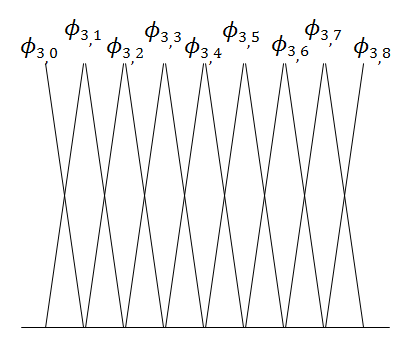
\includegraphics[width =\textwidth]{/NodalBasisLevel3.png}
	    %\vspace{3em}
		\centering
        \caption{Nodal basis}
    \end{subfigure} 
    \begin{subfigure}[b]{0.49\textwidth}    
	    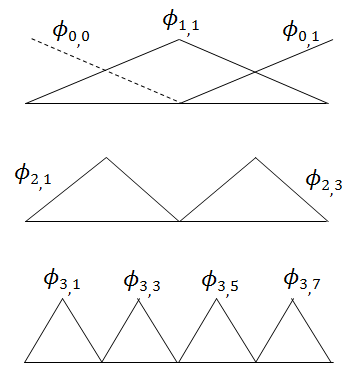
\includegraphics[width =\textwidth]{/HierBasisLevel3.png}
		\centering    
	 \caption{Hierarchical basis}
    \end{subfigure} 
    \caption{Nodal and hierarchical basis of level $n=3$. }
    \label{fig:NodalHierBasisLevel3}
\end{figure}		

\section{Sparse Grids based on hierarchical subspace splitting}
 Efficient discretization techniques are imperative for majority of problems in numerical mathematics such as interpolation, point approximation etc. Introduced by Zenger in \cite{Zenger1990} and based on hierarchical tensor product approximation spaces, sparse grids provide an efficient approach to improve the ratio of invested storage and computing time to the achieved accuracy.\cite{Bungartz1998}\\
  Following \cite{Zenger1990} finite element space is the direct sum of the subspaces where the error propagation is equal or larger than some prescribed tolerance. This leads to an approximation space that corresponds to a sparse grid in place of a full grid.\\
Hierarchical basis functions with small support and small contribution to function representation are not included in discrete space level n .This type of grids are classisified as sparse grids. 
%equation15 
\begin{equation}
    V_{n}^s := \bigoplus_{|\underline{l}|_1\le n} W_{\underline{l}}
\end{equation}
Using \eqref{eq9}, we get 
%equation16
\begin{equation}
    f_{n}^s \left(\underline{x}\right) 
    = \sum_{|\underline{l}|_1\le n} \sum_{|\underline{j}|\in B_{\underline{l}}} \alpha_{\underline{l},\underline{j}}\phi_{\underline{l},\underline{j}}\left(\underline{x}\right) 
    = \sum_{|\underline{l}|_1\le n} f_{\underline{l}}(\underline{x}), \quad \text{with} \ f_{\underline{l}} \in W_{\underline{l}}
\end{equation}

The sparse grids can also be formulated as follows:
%equation17
\begin{equation}
    V_{0,n}^s := \bigoplus_{|\underline{l}|_1\le n+d-1} W_{\underline{l}}, \quad l_t > 0
\end{equation}

The approximation error can defined as
%equation18
\begin{equation}
	\parallel f - f_{0,n}^s \parallel \le \sum_{|\underline{l}|_1\le n+d-1} \parallel f_{\underline{l}}\parallel
\end{equation}

where as the interpolation error is defined as 
%equation19
\begin{equation}
	{\parallel f - f_{n}^s \parallel}_{2} = \mathcal{O}\left(h_n^2\log{}(h_{n}^{-1})^{d-1} \right)
\end{equation}

\section{Combination technique}
To discretize a function $f$ on particular combination of anisotropic grids $\Omega_{\underline{l}}$ with uniform mesh size $h_{t} = 2^{l_{t}}$ in the t-th coordinate direction.  different grids have different mesh sizes for different directions. 
all grids can be considered with
%equation20
\begin{equation}
	|\underline{l}| := l_1 + ... + l_d = n-q, \ \ q = 0,...,d - 1, \ \ l_t \ge 0
\end{equation}

Using finite element approach with piece-wise linear function in each dimensions, one gets the nodal basis as discrete partial functions from different grids using the combination formula
%equation21
\begin{equation}
	f_n^c(\underline{x}) := \sum_{q=0}^{d-1}(-1)^q \left( \begin{array}{c}
	d-1 \\
	q  \end{array} \right) \sum_{|\underline{l}|_1=n-q} f_{\underline{l}}(\underline{x})
\end{equation}
The function $f_n^c(\underline{x})$ is a part of the sparse grid scpace $V_{n}$ .
%equation22
\begin{equation}
	|f-f_n^c| = \mathcal{O}\left(h_n^2 \cdot \log(h_{n}^{d-1}) \right)
\end{equation}

One can also consider ANOVA representation in form the combination method, where the function can be represented as
%equation23
\begin{equation}
	f(\underline{x}) = \sum_{\{j_1,...,j_q\}\subset\{1,...,d\}} c_{j_1,...,j_q} f_{j_1,...,j_q} \left( x_{j_1},...,x_{j_q} \right)
\end{equation}
where each $f$ depends only depends only on a subset of size $q$ of the dimensions. It is also possible that there exist different refinement levels for each dimension. If dimension $q$ is significantly smaller than $d$, then the complexity is only dependent on $q$, which is also called superposition dimension. An advantage of such case is beneficial where one can choose grids of their own and not follow the grid sequence.. This is known as the dimension adaptive procedure. Here an index set $I$ is expressed such that one needs to fulfill an admissibility condition
%equation24
\begin{equation}
	\underline{k} \in \text{I} \ \ \text{and} \ \ \underline{j}\le \underline{k} \quad \implies \quad \underline{j}\in \text{I}
\end{equation}
It means that index $\underline{k} \in I$ if all smaller grids belong to $I$. The combination coefficients for dimension adaptive combination technique depends only upon the index set $I$. 
%equation25
\begin{equation}
    f_I^c\left(\underline{x}\right) := \sum\limits_{\underline{k} \in I}\left( \sum\limits_{\underline{z} = \underline{0}}^{1}\left(-1\right)^{\left|\underline{z}\right|1}\cdot \chi^{I}\left(\underline{k}+\underline{z}\right)\right)f_{k}\left(x\right)
\end{equation}
where $\chi^{I}$ is the characteristic function of I and is expressed as follows
%equation 26
\begin{equation}
     \chi^{I}(\underline{k}) =
     \begin{cases}
        1 &  \text{ if } k \in I\\
        0 & otherwise 
     \end{cases}
\end{equation}

\section{Combination Technique}
Another motivation for sparse grids is to represent any sparse grid function as a linear combination of its interpolants on the regular full grids. This requires us to seek a certain linear combination of full grid spaces to create a sparse grid space. This approach do away with the need for data structures more complicated than a few arrays to store a sparse grid function and requires only regular data structures.\cite{Griebel1992b} \\
The crux of the combination technique is similar to the multilevel splitting of the finite element spaces which changes the nodal bases of the space with hierarchical bases. \cite{Yserentant1986} The basis for combination techniques comes from the liner combination of independent solution of many problems with reduced size. \cite{Griebel1992}. Figure \ref{fig:Sparsegrid} shows an example of this multilevel combination which is basically addition and subtraction in this special case.

		\begin{figure}
			\centering
			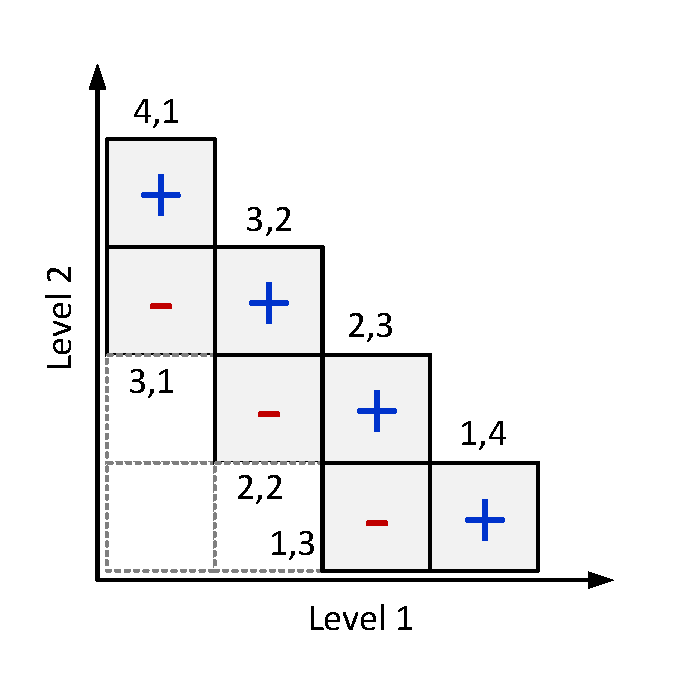
\includegraphics[width=0.6\textwidth]{/SparseGrid.pdf}
			\caption{Classical sparse grid combination method for l=4}
			\label{fig:Sparsegrid}
		\end{figure}

In total combination technique involves $O({h}^{-1}_nlog({h}^{-1}_n))$  unknowns in contrast to $O({h}^{-2}_n) $ unknowns for the conventional full grid approach however combination solution is nearly as accurate as the standard solution. it can be proven that error is only slightly worse than for the associated full grid.\cite{Griebel1992a, Griebel1992b}. To some extent the combination technique even works for non-smooth solutions. Now, ${h}^2_i$ and ${h}^2_j$ in have to be replaced by ${h}^\alpha_i$ , ${h}^\beta_j$ with appropriate $\alpha$ and $\beta$, but because of the properties of the combination technique the leading error terms still cancel. However, for the problems with severe singularities, the appropriate combination of adaptively refined grids is recommended.\cite{Griebel1992a}\\ It is seen that in some situations the combination technique leads to the cancellation of certain error terms in the asymptotic error expansion\cite{Griebel1992b} \\
 Lastly, one should note that the error analysis of this method has been relatively explained in \cite{Garcke2013} and the references there within. For further details please check the chapters of related works under "Works on Error Analysis and Convergence" presented earlier in the thesis. The discussion of these analysis is out of scope for this thesis but perhaps relatively important in future works.
%
%\section{Some General Discussions and Points}
%1. The resulting algorithm can be used as a solver and within a preconditioner. it can also be applied as a preconditioner for the full grid problem to speed up a basic iterative solver. \cite{Griebel1992} \\
%
%\subsection{Argument of error and convergence}
%1. We show that the condition number of such a stiffness matrix for multilevel splitting of finite element spaces behaves like $O((log \kappa)^2) $ where $\kappa$ is the condition number of the stiffness matrix with respect to a nodal basis. \cite{Yserentant1986} \\
%2. error satisfies $O({h}^2_nlog({h}^{-1}_n))$ (pointwise and with respect to the $L_2$- and $L_\infty$-norm).\cite{Griebel1992b} \\
%
%3. For the Poisson equation on the unit square it is proved that the combined solution converges with order $O(h)$ in the energy norm and with order $O(h^2log h)$ in the $L^2$-norm. (journals 5 and 9 are very similar aka poisson vs. second-order elliptic differential equations-9 general of 5) \cite{Pflaum1993}\\
%
%\subsection{Argument of Preconditioner plus solver}
%1. The resulting algorithm can be used as a solver and within a preconditioner. it can also be applied as a preconditioner for the full grid problem to speed up a basic iterative solver. \cite{Griebel1992} \\
%
%2. In addition to being a solver in its own right, the combination method can be used as a parallel preconditioner for the full grid problem. Then, a basic iterative method is accelerated substantially and shows nearly optimal, i.e. multigrid-like convergence behavior, if the accuracy of the solution is required only up to the truncation error.\cite{Griebel1992} \\
%
%\subsection{Argument of relation between hierarchical basis and nodal basis}
%1. As the representation of a finite element function with respect to a hierarchical basis can be converted very easily and quickly to its representation with respect to a nodal basis, our results mean that the method of conjugate gradients needs only logarithm of the dimension of the finite element space steps and computer operations to reduce the energy norm of the error by a given factor if one uses hierarchical bases or related preconditioning procedures. \cite{Yserentant1986} \\
%
%2.Two dimensional sparse grids contain only $O({h}^{-1}log({h}^{-1}))$ grid points in contrast to the usually used full $O({h}^{-2}) $ grids, whereas for a sufficiently smooth function the accuracy of the representation is only slightly deteriorated. from $O(h^2) $ to $O(h^{2}log({h}^{-1}))$. \cite{Griebel1992b} \\
%
%3. Using this type of hierarchical basis the calculation with functions defined on different grids and spaces is simplified. For example, the addition of two functions defined on different grids is reduced to the addition of the single coefficients. This is due to the fact that now the basis functions that are associated with the grid points which belong to both grids are just the same. \cite{Griebel1992b} \\
%
%4. The transformation of the coefficients of a function on grid represented in standard nodal basis to its representation in hierarchical basis can be implemented by a constant number of operations per grid point. The transformation to the hierarchical basis representation is done by the algorithm in \cite{Griebel1992b}. \\
%
%5. The advantage of using the hierarchical basis representation during the combination process is that no interpolation to additional grid points has to be performed explicitly: For each 'missing' grid point, the interpolated value would be zero in hierarchical basis representation, and thus can be omitted during the combination of solutions\cite{Griebel1995} \\
%
%6. One of the main advantages of hierarchical bases compared with standard nodal point bases is probably the fact that the basis gets a multilevel structure. Thus, we can now distinguish between high-level basis functions with a large support that usually (in the smooth case, at least) already contain a significant part of the information, and functions living on lower levels whose contribution to an interpolant or a finite element approximation is rather small. The decrease of the hierarchical coefficients from level to level can be used, of course, to control adaptive grid refinement, but, if it is combined with a tensor product approach for the higher dimensional case, it can be used for an a priori reduction of the number of grid points involved in the calculation, too.\cite{Bungartz1998}\\
%
%7. The hierarchical coefficient or hierarchical surplus itself can be used to indicate the smoothness of u at the corresponding grid point and, consequently, the necessity to refine the grid here.\cite{Bungartz1998}\\
%
%8. The elements of the sparse grid space can be represented in a hierarchical basis [27] and many algorithms for hierarchical basis methods including wavelets can be used for the solution [5,20]. Compared to the commonly used nodal basis, a hierarchical basis of, e.g. multilinear functions has its disadvantages, as the corresponding matrices have reduced sparsity and a less regular structure. This is due to the fact that the supports of the lower level basis functions are large and intersect nontrivially with many higher level basis functions. These difficulties increase with dimension.
%An efficient way to avoid the problem of reduced sparsity is given by the combination technique. \cite{Hegland2007}\\

		
		
		
		%
		%% ---------------------------------------------------------------------------
		%%
		%% Fully Automated Calibration for Ultrasound
		%%
		%%% ---------------------------------------------------------------------------
		\part[Part Two: Implementation, Results and Conclusion]{Implementation, Results and Conclusion}
		\label{secondpart}
		\chapter{Current Implementation}
\label{chapter:myImplementation}

%1. for non smooth solutions and more complex problems theory is still missing. Here like for the standard grid adaptive refinement seems to be necessary to get around solution method. First attempts in this direction are promising\cite{Griebel1992b} \\
%
%2. Consequently, one of the main advantages of the combination technique stems from the properties of sparse grids [1] In comparison to the standard full grid approach the number of grid points can be reduced significantly. Another advantage has to be seen in the simplicity of the combination concept its inherent parallel structure and its framework property allowing the integration of existing solvers for partial differential equations.\cite{Bungartz1994}\\ % write however the idea is in some way different in current implementation
%
%3. we have implicitly assumed that this is the coarse mesh with spacing h that is naturally embedded in the fine mesh, so that the fine mesh solution may be transferred to the coarse mesh with injection.
%
%4. In elliptic problems the smoothness of the solution may be disturbed where the data is non-smooth. The form of the domain or the need for local refinement may make the use of uniform meshes difficult.  The local smoothness of the solution is a basic characteristic of many elliptic problems, so that extrapolation can be used locally, even when the global solution is non-smooth. With this background, several interesting new extrapolation-based approaches have been developed within the past few years, including the sparse grid combination technique and multivariate extrapolation. In this paper we will focus on explicit extrapolation methods that are based on the (linear) combination of solutions on different grids. Implicit extrapolation methods, in contrast, obtain higher order by applying the extrapolation idea on quantities like the truncation error or the numerical approximation of the functional. Such methods are discussed in Rude\cite{Rude1994, Rude92extrapolationand} \\
%
%5. Using bilinear interpolation for each single component function, we can extend the the domain of definition to the union of all participating grids. This is possible, because bilinear interpolation can be shown to be compatible with the error splitting.\cite{Rude1994} \\
%
%6. Obviously, an algorithm is needed which combines the advantages of both methods: low storage requirements, a low number of operations involved, but still simple data structures. In the following, we present an algorithm that fulfills these requirements\cite{Griebel1995} \\
%
%7. Firstly, the block structure of a grid reduces main memory requirements. In an inner iteration step, the problem is solved one block at a time. An outer iteration establishes the overall solution. Secondly, the block structure of a grid is a natural basis for the parallelization of the solver. Each processor solves the problem on one of the blocks, and communication is necessary merely along block interfaces, in order to achieve a smooth solution on the whole domain.\cite{Griebel1995} \\
%
%8. The hierarchical coefficient or hierarchical surplus itself can be used to indicate the smoothness of u at the corresponding grid point and, consequently, the necessity to refine the grid here.\cite{Bungartz1998}\\
 
 \section{General Ideas}
 
 		
		Productivity experts claim that breakthroughs come by thinking "nonlinearly". Tree structures have been an enormous leap in data organization since they allow the implementation of algorithms more rapidly than linear data structures such as lists, vectors and sequences.
		
		In categorizing trees as "nonlinear" with respect to organizational relationship, the main feature that must be highlighted is more sophisticated relationships than elementary "before" and "after" relationships between objects in sequences. A tree follows a \textbf{hierarchical} architecture, with some objects being "above" and some "below" others.
		
		A \textbf{tree} is an abstract data type. In a tree, each element has a \textbf{parent} element. It can have zero or more \textbf{children} elements.
		\\
		\textbf{Formal Tree Definition}
		
		A \textbf{tree T} can be defined as a set of \textbf{nodes} storing elements in a \textbf{parent-child} relationship and has the properties as defined below:
		\begin{itemize}
			\item A nonempty \textbf{T} has a special node known as the \textbf{root} of \textbf{T} which has no parent. 
			\item Every other node \textit{$\nu$} of \textbf{T} has a unique parent node \textit{w} and every node with parent \textit{w} is a \textbf{child} of \textit{w}.
		\end{itemize}

		If a parent has two nodes which are its children, then these children are \textbf{siblings}. If a node \textit{$\nu$} does not have children then it is \textbf{external} while it is \textbf{internal} if it has one or more children. External nodes can also be termed as \textbf{leaves}.
		
		Figure \ref{fig:GeneralTree} shows an example of a tree representing computer files organized in the form of nested directories. 
		
		\begin{figure}[h]
			\centering
			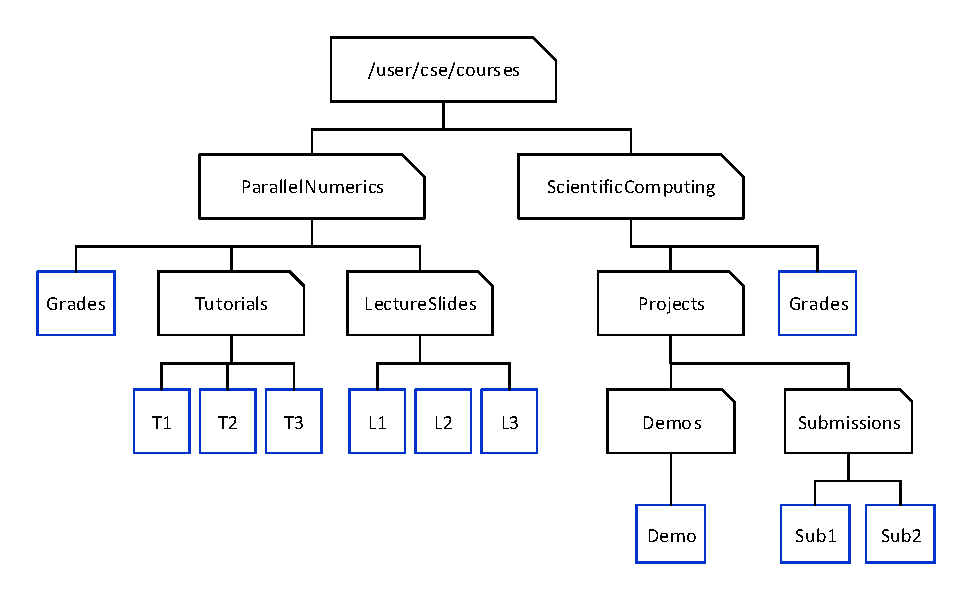
\includegraphics[width=\textwidth]{/GeneralTree.pdf}
			\caption{Tree representing a portion of a file system}
			\label{fig:GeneralTree}
		\end{figure}
		
		\textbf{Ordered Trees}
		
		A tree having a linear ordering for the children of each node is termed as \textbf{ordered}. The children of a node  can be identified as first, second and so on. In ordered trees, linear order relationship between siblings is illustrated by listing them in a sequence.
		
		For implementation "position" and "node" can be used interchangeably for trees. \\
		
		\textbf{A Linked Structure for General}
		
		A \textbf{linked structure} can be used to comprehend a tree \textbf{T}. Each node of \textbf{T} can be depicted as a position object \textit{p} with the below mentioned fields:
		reference to the node's element, link to node's parent and some kind of collection to store links into node's children.  Figure \ref{fig:LinkedStrucGenTree} shows a representation of  a node of a tree and a schematic representation of the data structure associated with a node and its children. \\
		
		% The height of a tree is equal to the maximum depth of its external nodes.
		\begin{figure}[h]
			\centering
		    \begin{subfigure}[b]{0.33\textwidth}
			    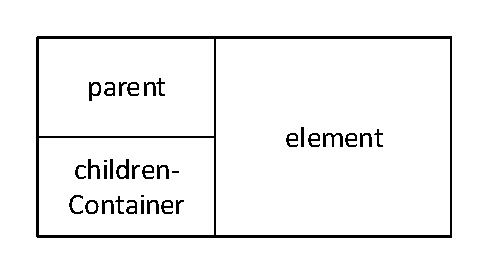
\includegraphics[width =\textwidth]{/LinkedStrucGenTree1.pdf}
			    %\vspace{3em}
				\centering
		        \caption{}
		    \end{subfigure} 
		    \begin{subfigure}[b]{0.66\textwidth}    
			    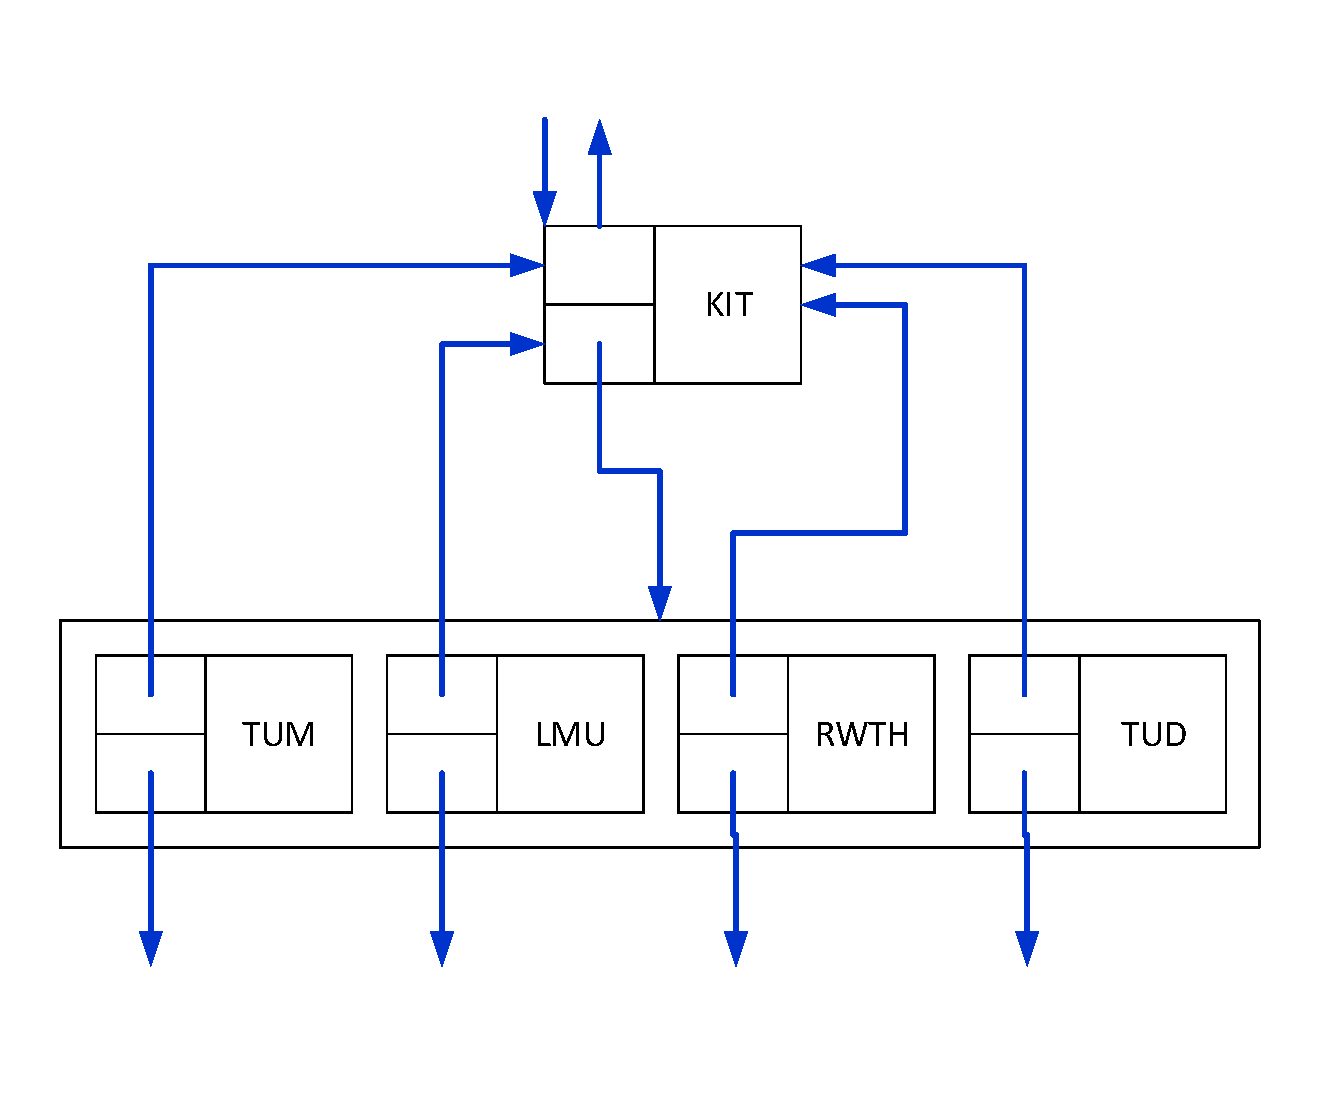
\includegraphics[width =\textwidth]{/LinkedStrucGenTree2.pdf}
				\centering    
			 \caption{}
		    \end{subfigure} 
		    \caption{The linked structure for a general tree: (a) the node structure; (b) the portion of the data structure associated with a node and its children.}
		    \label{fig:LinkedStrucGenTree}
		\end{figure}
		
		
		\textbf{Preorder Traversal}
		
		A traversal of a tree \textbf{T} is a method of acquiring all the nodes of \textbf{T}. Preorder traversal which is a basic traversal scheme for trees has been represented here.\\
		In a preorder traversal of \textbf{T}, the root of \textbf{T} is called initially and further the subtrees rooted at its children are traversed repeatedly. In an ordered tree, the subtrees are traversed according to the order of the children. The definitive action associated with the "visit" of a node depends on the application of this traversal.\\
		
		\textbf{Algorithm}  preorder(T, p):\\
		perform the "visit" action for node p\\
		for each child q of p do\\
		recursively traverse the subtree rooted at q by calling preorder (T,q)\\ 
		
		This algorithm is suitable for creating a linear ordering of the nodes of a tree in which parents always come before their children.\\
		
		The preorder traversal is an effective way to access all the nodes of a tree.\\
		
		Figure \ref{fig:TransversalOrderedTree} shows an example of the preorder traversal of the tree associated with a research paper. The document is sequentially read from beginning to the end.
		
				\begin{figure}[h]
				\centering
					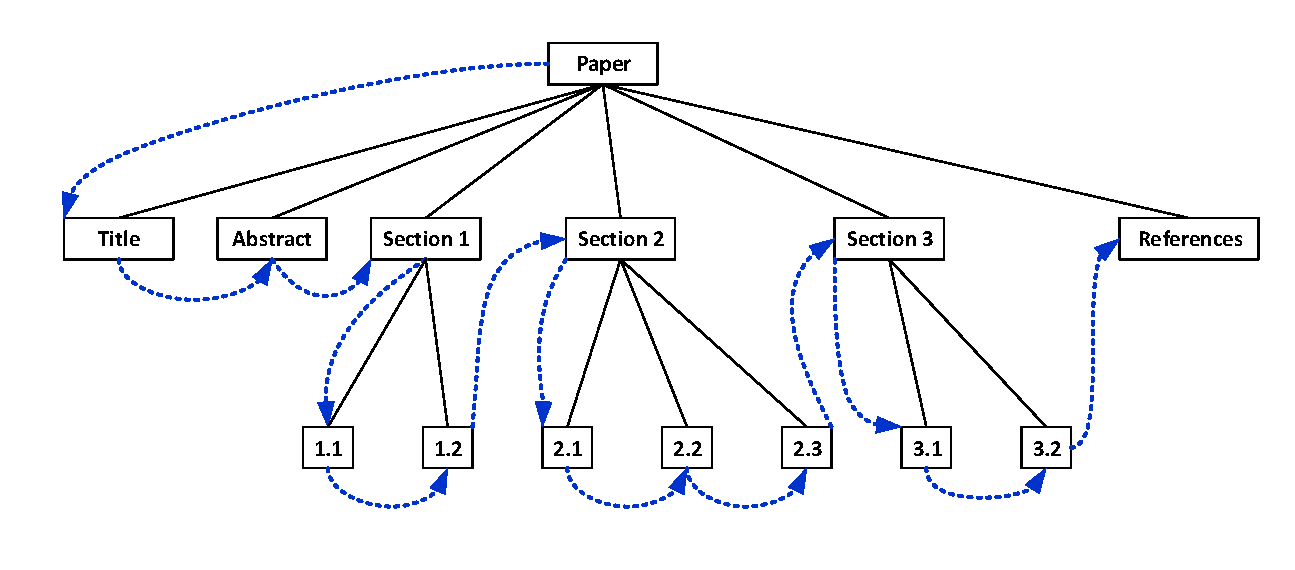
\includegraphics[width=\textwidth]{/TransversalOrderedTree.pdf}
					\caption{Preorder traversal of an ordered tree, where the children of each node are ordered from left to right.}
					\label{fig:TransversalOrderedTree}
				\end{figure}
		
		\textbf{Quad Trees}\\
		
		A \textbf{quad tree} is an ordered tree in which each node has at most four children
		\begin{enumerate}
			\item Every node has at most four children.
			\item Each child node can be labeled as south-west(SW), south-east(SE), north-west(NW) or north-east(NE).
			\item The ordering of a node is implemented as SW$\rightarrow$SE$\rightarrow$NW$\rightarrow$NE. 
		\end{enumerate}
		A quad tree is termed to be \textbf{proper} if each node has either zero or four children.\\
		
		\textbf{A Recursive Quad Tree Definition}\\
		A recursive quad tree can be defined as a quad tree which
		\begin{itemize}
			\item is either empty
			\item consists of a node which is \textbf{root} and four further quad trees which are called as south-west(SW), south-east(SE), north-west(NW) or north-east(NE) subtrees. 
		\end{itemize}
		 
		 Figure \ref{fig:NodeQuadTree} shows a representation of a node in a linked data structure for representing a quad tree.
		 		
		 \begin{figure}[h]
		 	\centering
		 	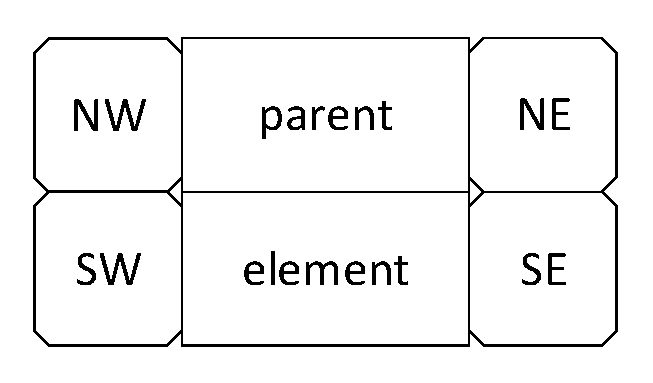
\includegraphics[width=0.33\textwidth]{/NodeQuadTree.pdf}
		 	\caption{A node in a linked data structure for representing a quad tree.}
		 	\label{fig:NodeQuadTree}
		 \end{figure}

 
 \section{Different Schemes}
 



		\chapter{Results}
\label{chapter:results}
In this chapter the result of the current implementation will be presented and discussed in details to have an insight of the important observable issues. Trying to tackle the different schemes and naturally compare it to a full grid method is the primary objective here. \\

%%%The problem at hand might seem very trivial at first as the interpolation problem is being investigated in two dimensions. However, the flexibility and robustness of the implementation shows how it can easily be extended to the higher dimension. It is also how a complex data structure has been implemented to give a proper base for future works.\\

In addition, not only the solution at hand is the base for higher dimension, it can also be a base for different applications, such as regression and data fitting problem in data mining, preconditioner for multigrid-like methods, partial differential equation solver in elliptic and parabolic problems, and more importantly in computational mechanics, chemistry or physics. However, by realizing this hierarchy of complexity of problems, it can be observed that interpolation problem is the fundamental method which is the task discussed here. The author acknowledges the drawbacks of method mainly in regard to convergence, but also addresses the reasons which could resolve a part of those problems for the current implementation.\\

As discussed earlier in chapter \ref{chapter:myImplementation}, the objective here is to project the result of the combination technique to the full grid. This has already been done by the fact that the underlying idea of the current implementation is to first project the function values of different level vector grids all to be combined with into a corresponding full grid and then combine them pointwise. This way some advantages and some disadvantage compared to other combination schemes presented in the literature can be observed. \\

Firstly, the obvious disadvantage would be the fact that by projection of all grids to a full grid requires a lot of extra memory consumption and this is exactly against the idea of rectifying curse of dimensionality. However, a solution is described here to address this problem, which will be better observed after the examination of the results of the adaptive refinement strategy. Assuming the method works for the adaptive refinement, it gives the rise to idea that it is required to use a coarse grid and use adaptive refinement in the areas needed. This way, total error of same order will be achieved with less storage and operations in comparison to full grid which needs high resolution in the first place. In the worst case scenario, the full grid resolution will be achieved and the solution structure requires exactly the number of grids in combination technique scheme multiplied by the storage required for the normal full grid. Since high valued level vector is not used in this case, it is not a significant weakness.\\

In contrast, the advantage that can be achieved in this method is that while the required tasks performed separately for each of the grids in the implemented version of combination method is same as normal combination technique, the extra effort is just from a projection. Therefore, using a very efficient projection method, there are not many operations added to the solution which ultimately means less computational effort compared to solution on normal full grid method. Another advantage of this, as discussed earlier, can be possibility to start with a coarse grain solution and adaptively refine to areas needed. A detailed investigation of using lower resolution schemes for lower subtree problems can possibly show better result for storage space and memory usage. \\

Note that conventionally we are using the unit square domain as shown in figure \ref{fig:results1Square}. The reason for this is that mathematically, the division of square domain is easier and straightforward. However, our implementation can work with any rectangular domain as shown in an example in figure \ref{fig:results1Rect}. 

%1figure rectangle and figure square together
\begin{figure}[h]
	\centering
    \begin{subfigure}[b]{0.49\textwidth}    
	    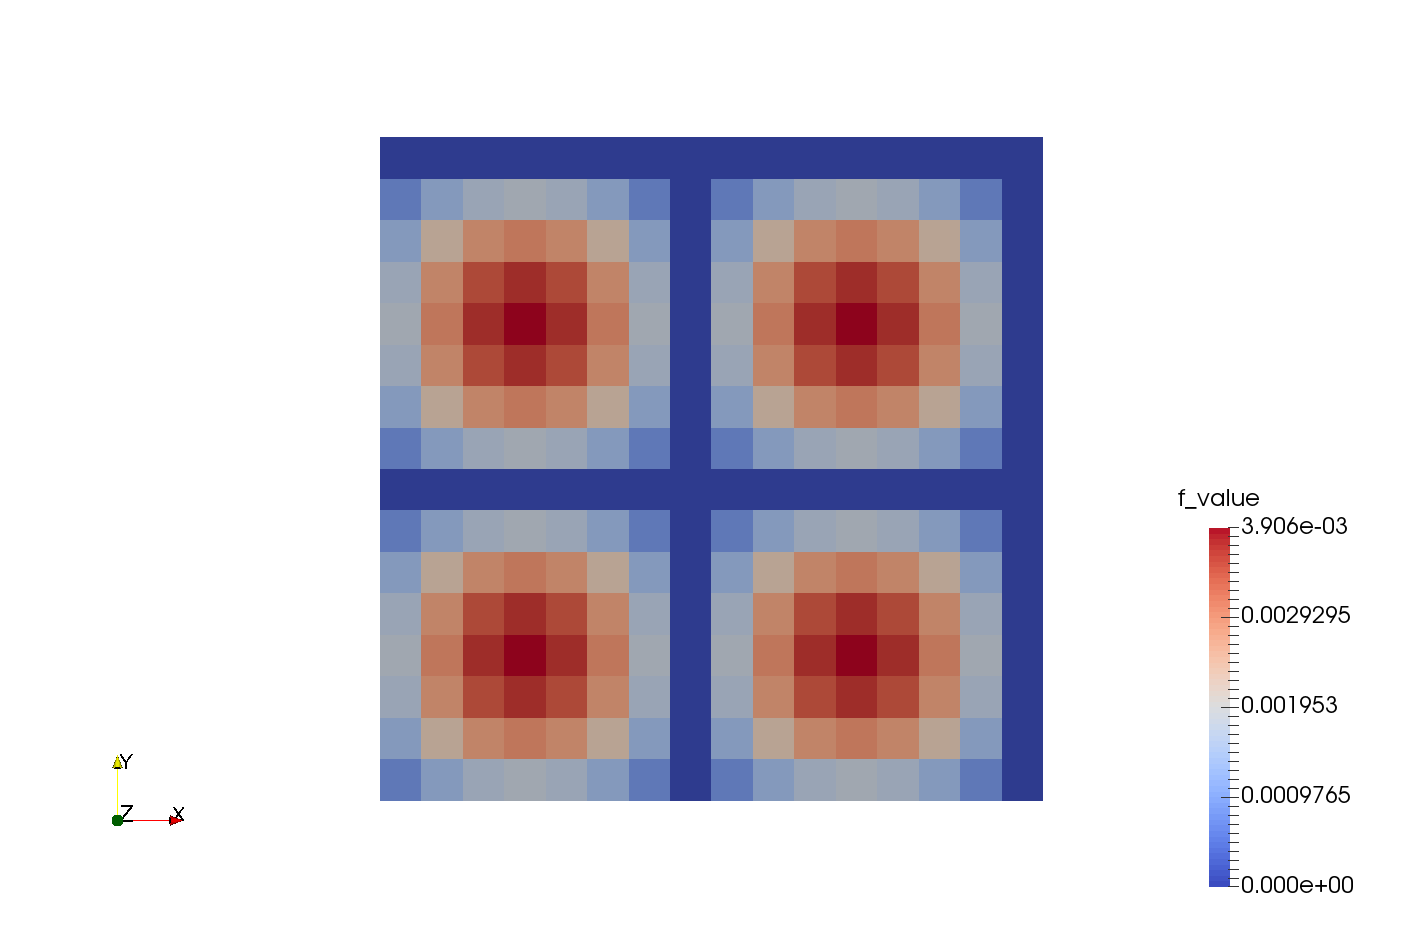
\includegraphics[width =\textwidth]{/results/1/square.png}
		\centering    
	 \caption{}
	 \label{fig:results1Square}
    \end{subfigure} 
    \begin{subfigure}[b]{0.49\textwidth}
	    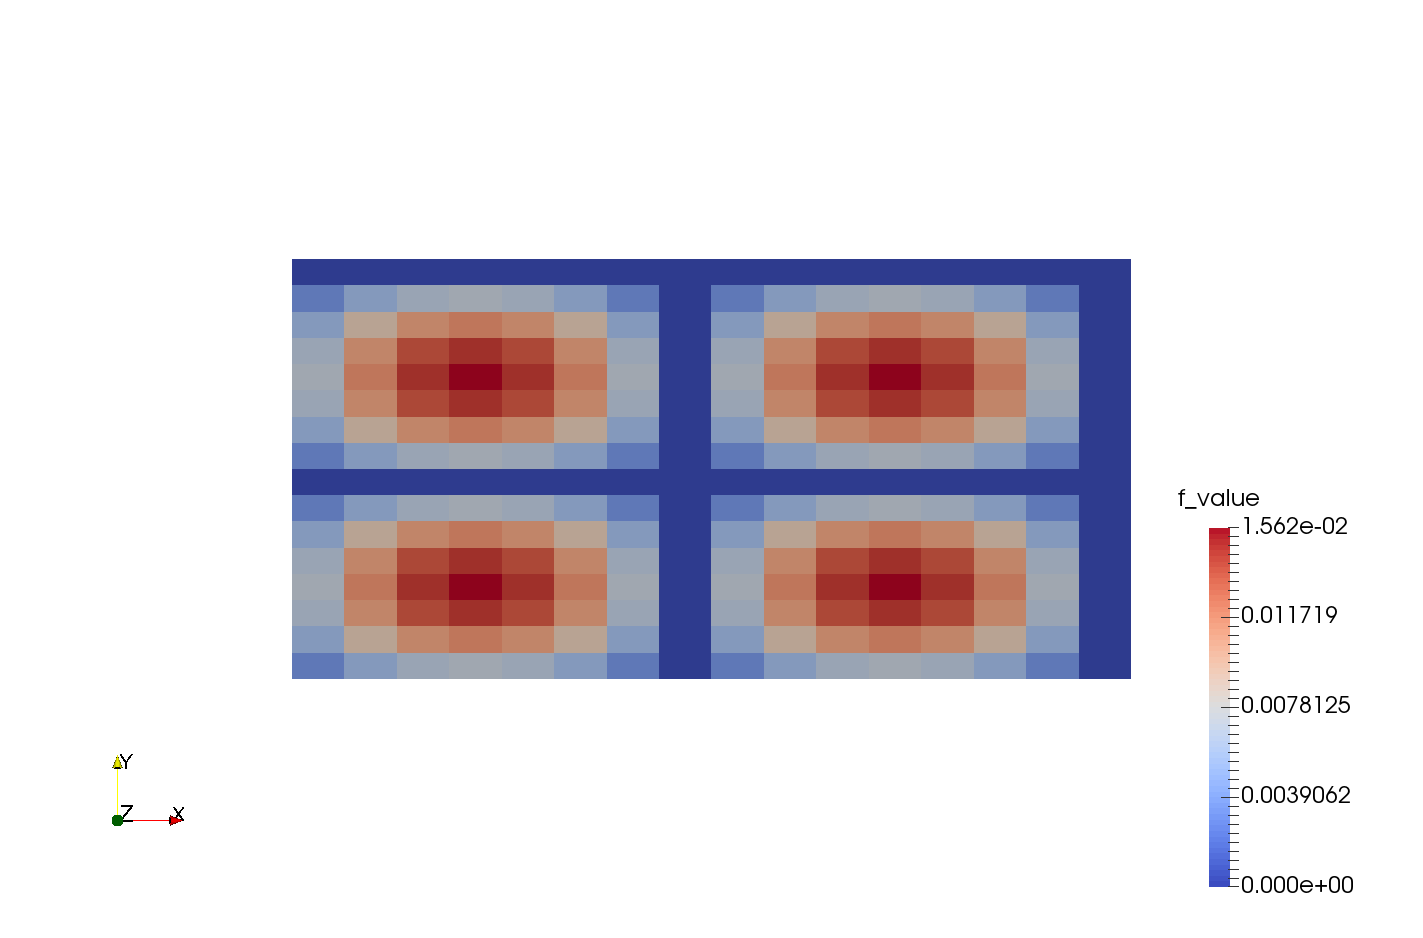
\includegraphics[width =\textwidth]{/results/1/rectangle.png}
	    %\vspace{3em}
		\centering
        \caption{}
        \label{fig:results1Rect}
    \end{subfigure}     
    \caption{The linked structure for a general tree: (a) the node structure; (b) the portion of the data structure associated with a node and its children.}
    \label{fig:results1SquareRect}
\end{figure}

\section{Verification of components}
In any case, as for any scientific approach, we first need to verify that our implementation works as expected. This has been done by comparison of the solution to normal full grid problem. We present here different test cases to ensure the functionality under a variety of cases.
\begin{enumerate}
\item $f(x)=x^2+y^2$
\item $f(x)=x^2 \cdot y^2 $
\item $f(x)=\sqrt[2]{x} \cdot \sqrt[2]{y}$
\item $f(x)=16 \cdot x(1-x)y(1-y)$
\end{enumerate}
In each case we try to compare the error of combination technique, given the default scheme of $\overrightarrow{l}=(4,4)$.\\

In every case, the figures showing the difference are compiled in figure \ref{fig:results2case1-4Diff} to better observe and compare the extent of the spread of error in the domain. For special test case 1, the results are shown in figure \ref{fig:results2case1}. Since the bilinear interpolation is used in this case, figure shows that the combination technique gives the perfect solution. The reason for this is the nature of problem. Since bilinear interpolation is performed in one direction first and then in the other direction, it can be observe that interpolation of a function which is not of terms $x^even \cdot y^even$ gives no error. Figures \ref{fig:results2case2}-\ref{fig:results2case4} show the results for cases 2-4
%2figure case 1 verification difference, combigrid, fullgrid alll together
\begin{figure}[h]
	\centering
    \begin{subfigure}[b]{0.49\textwidth}
	    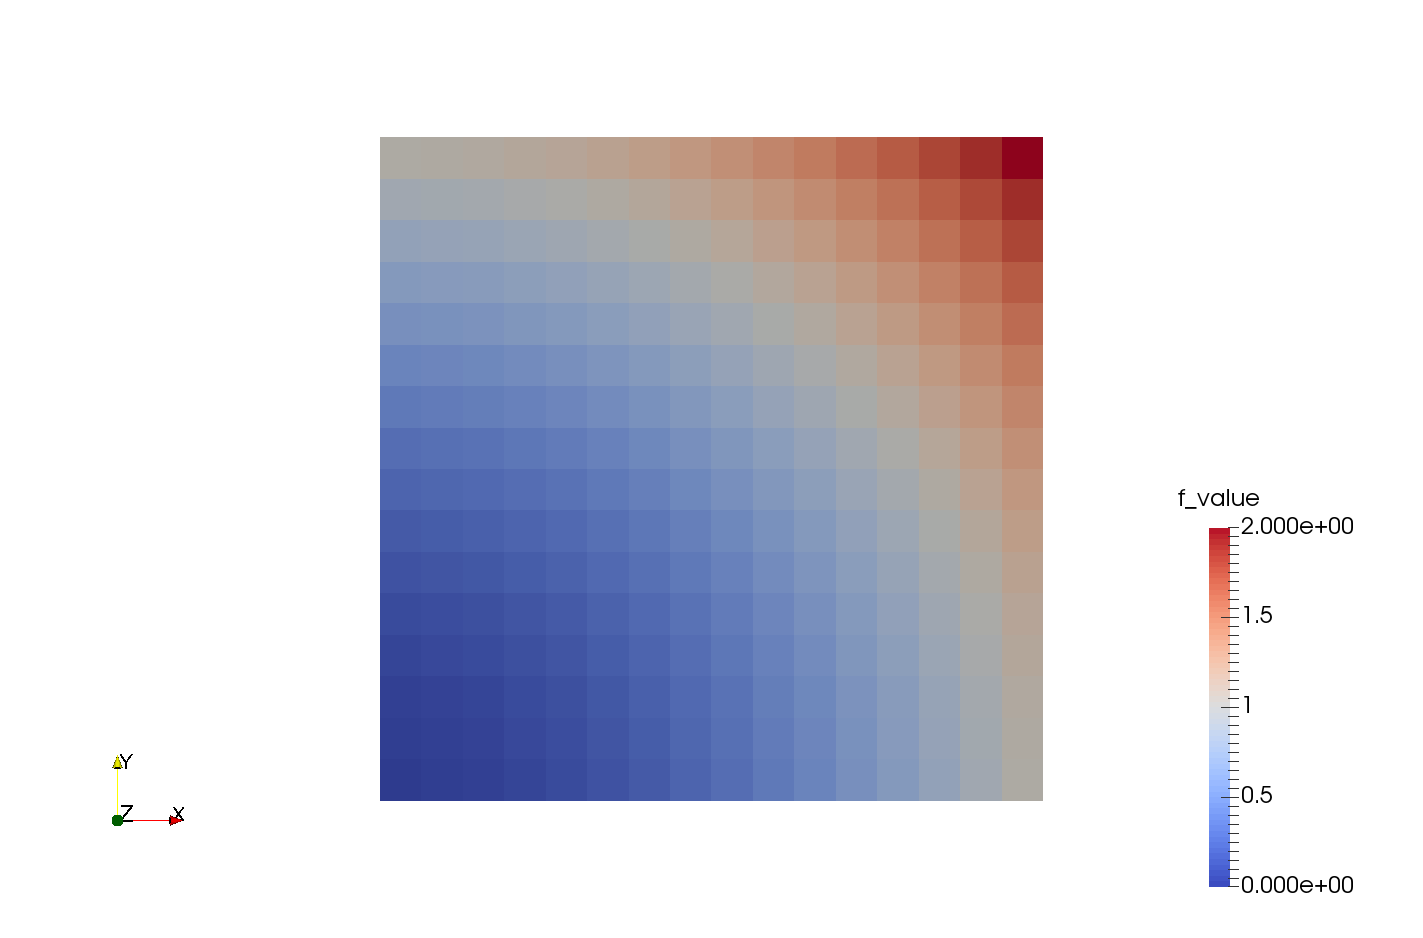
\includegraphics[width =\textwidth]{/results/2/case1-verification-combination.png}
	    %\vspace{3em}
		\centering
        \caption{Combination}
        \label{fig:results2case1Combi}
    \end{subfigure} 
    \begin{subfigure}[b]{0.49\textwidth}    
	    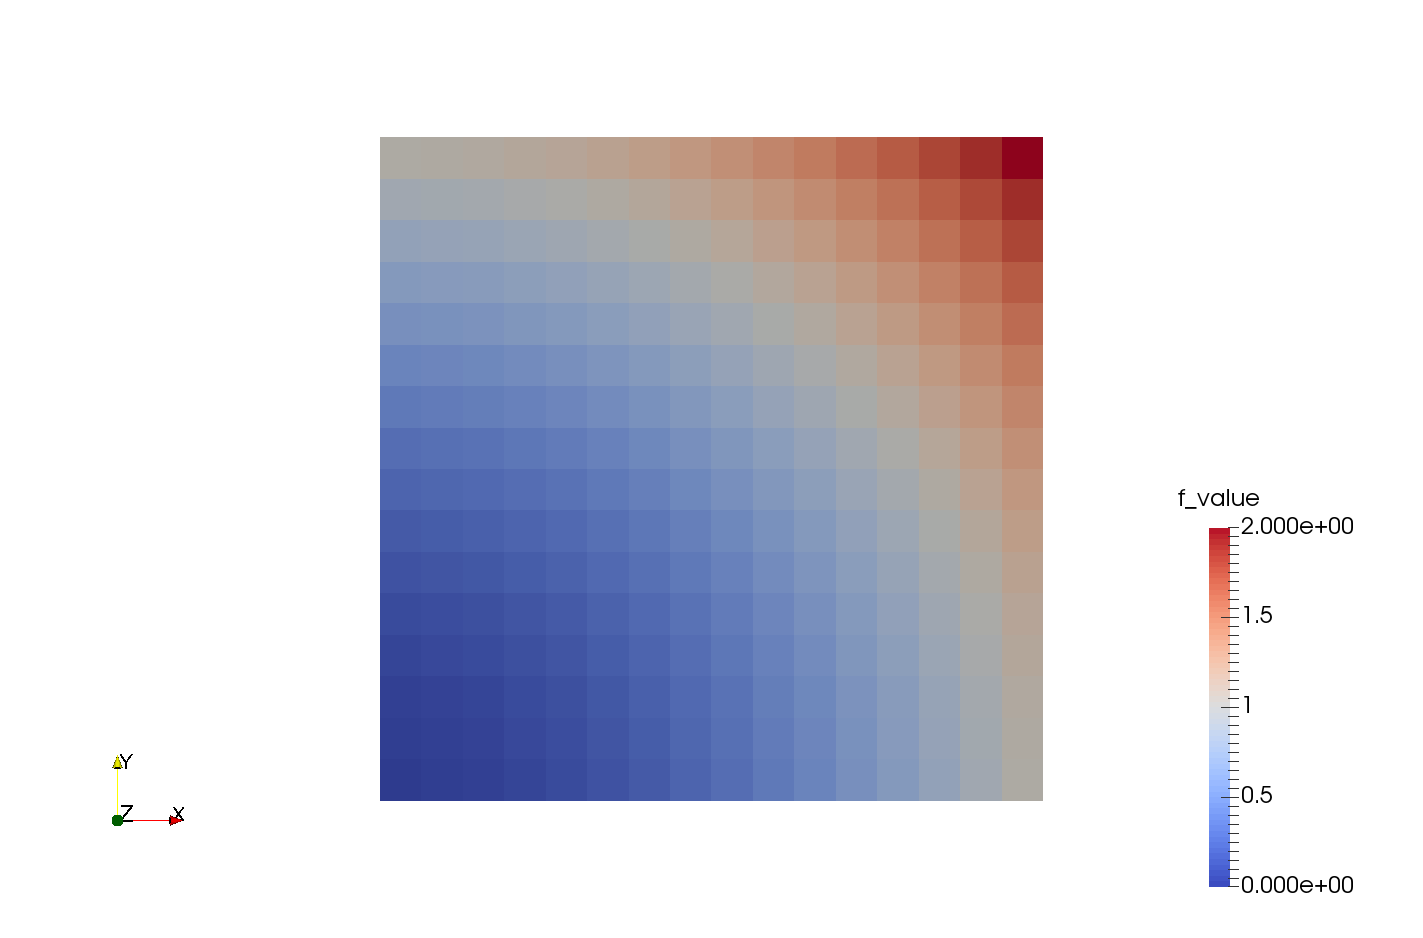
\includegraphics[width =\textwidth]{/results/2/case1-verification-fullgrid.png}
		\centering    
		 \caption{Verification}
	    \label{fig:results2case1Full}	 
    \end{subfigure} 
    \caption{(a) Combination and (b) verification for case 1}
    \label{fig:results2case1}
\end{figure}
%2figure case 2 verification difference, combigrid, fullgrid alll together
\begin{figure}[h]
	\centering
    \begin{subfigure}[b]{0.49\textwidth}
	    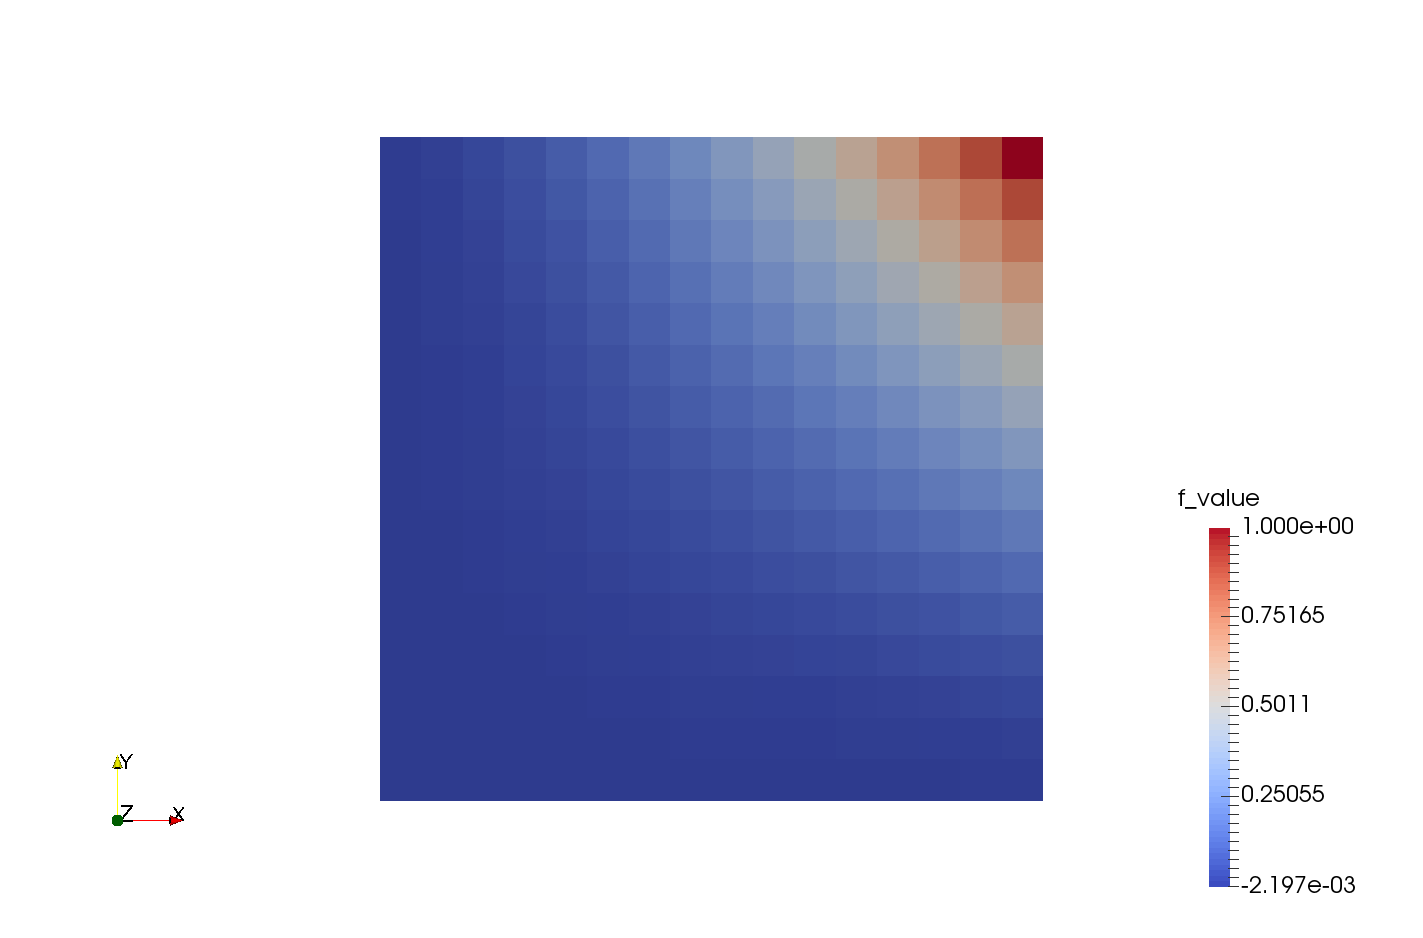
\includegraphics[width =\textwidth]{/results/2/case2-verification-combination.png}
	    %\vspace{3em}
		\centering
        \label{fig:results2case2Combi}
        \caption{Combination}
    \end{subfigure} 
    \begin{subfigure}[b]{0.49\textwidth}    
	    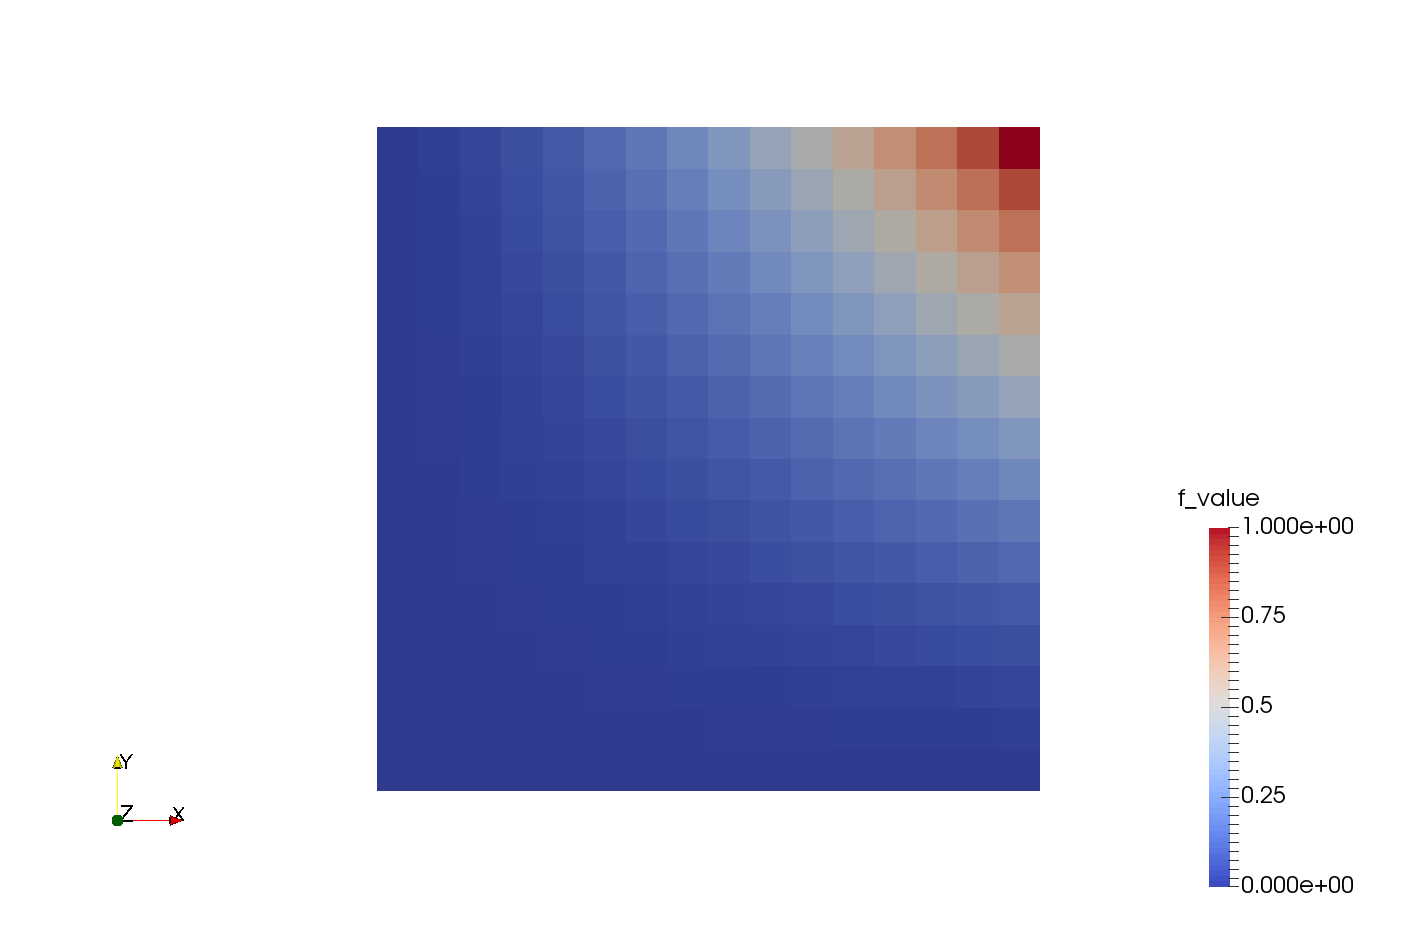
\includegraphics[width =\textwidth]{/results/2/case2-verification-fullgrid.png}
		\centering    
	 \caption{Verification}
	    \label{fig:results2case2Full}	 	 
    \end{subfigure} 
    \caption{(a) Combination and (b) verification for case 2}
    \label{fig:results2case2}
\end{figure}
%2figure case 3 verification difference, combigrid, fullgrid alll together
\begin{figure}[h]
	\centering
    \begin{subfigure}[b]{0.49\textwidth}
	    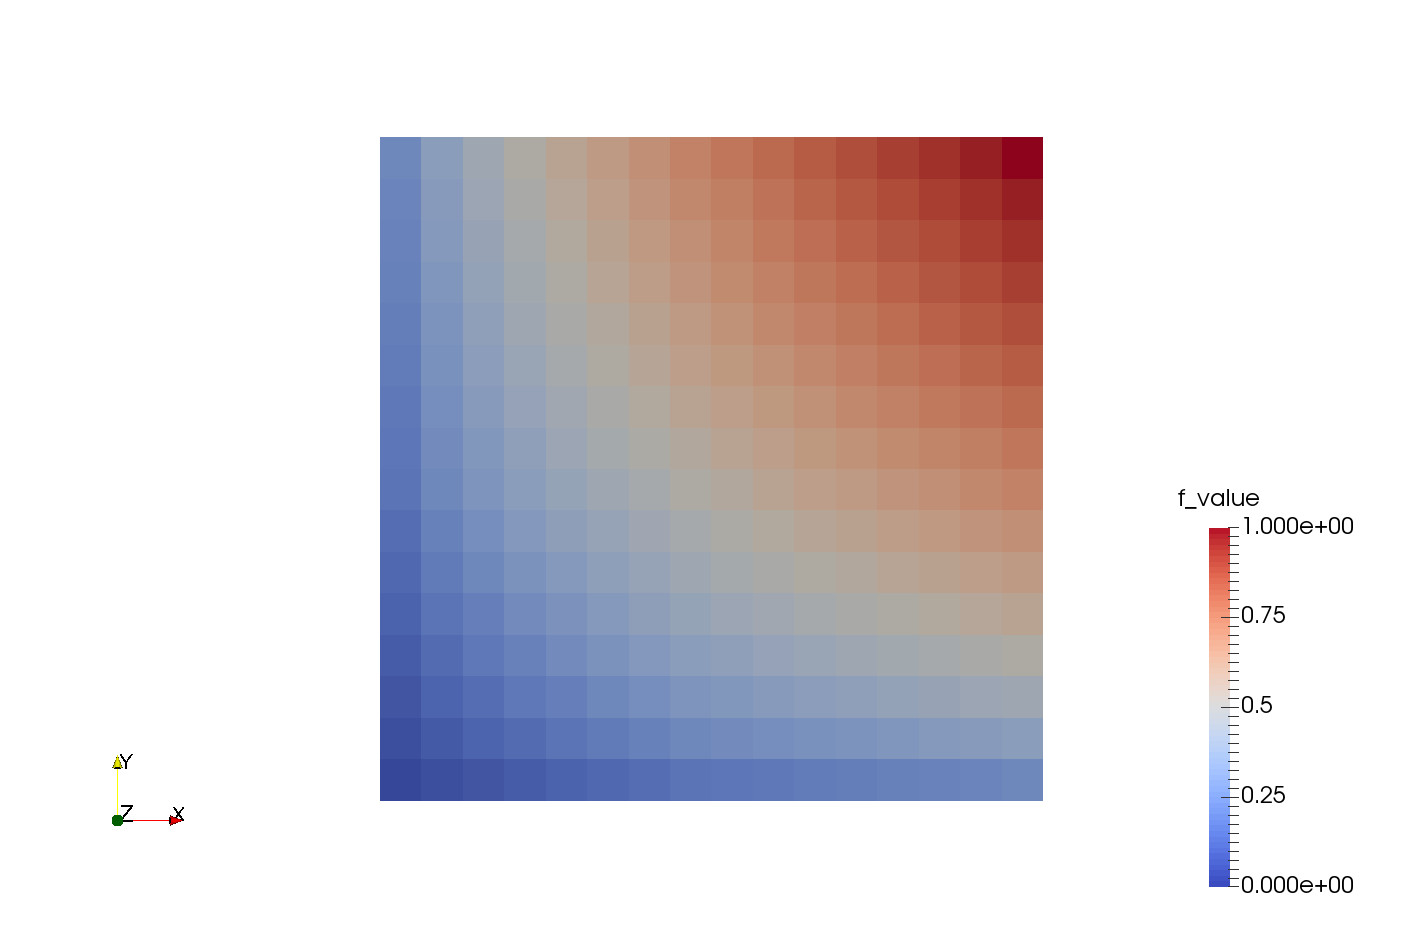
\includegraphics[width =\textwidth]{/results/2/case3-verification-combination.png}
	    %\vspace{3em}
		\centering
        \label{fig:results2case3Combi}
        \caption{Combination}
    \end{subfigure} 
    \begin{subfigure}[b]{0.49\textwidth}    
	    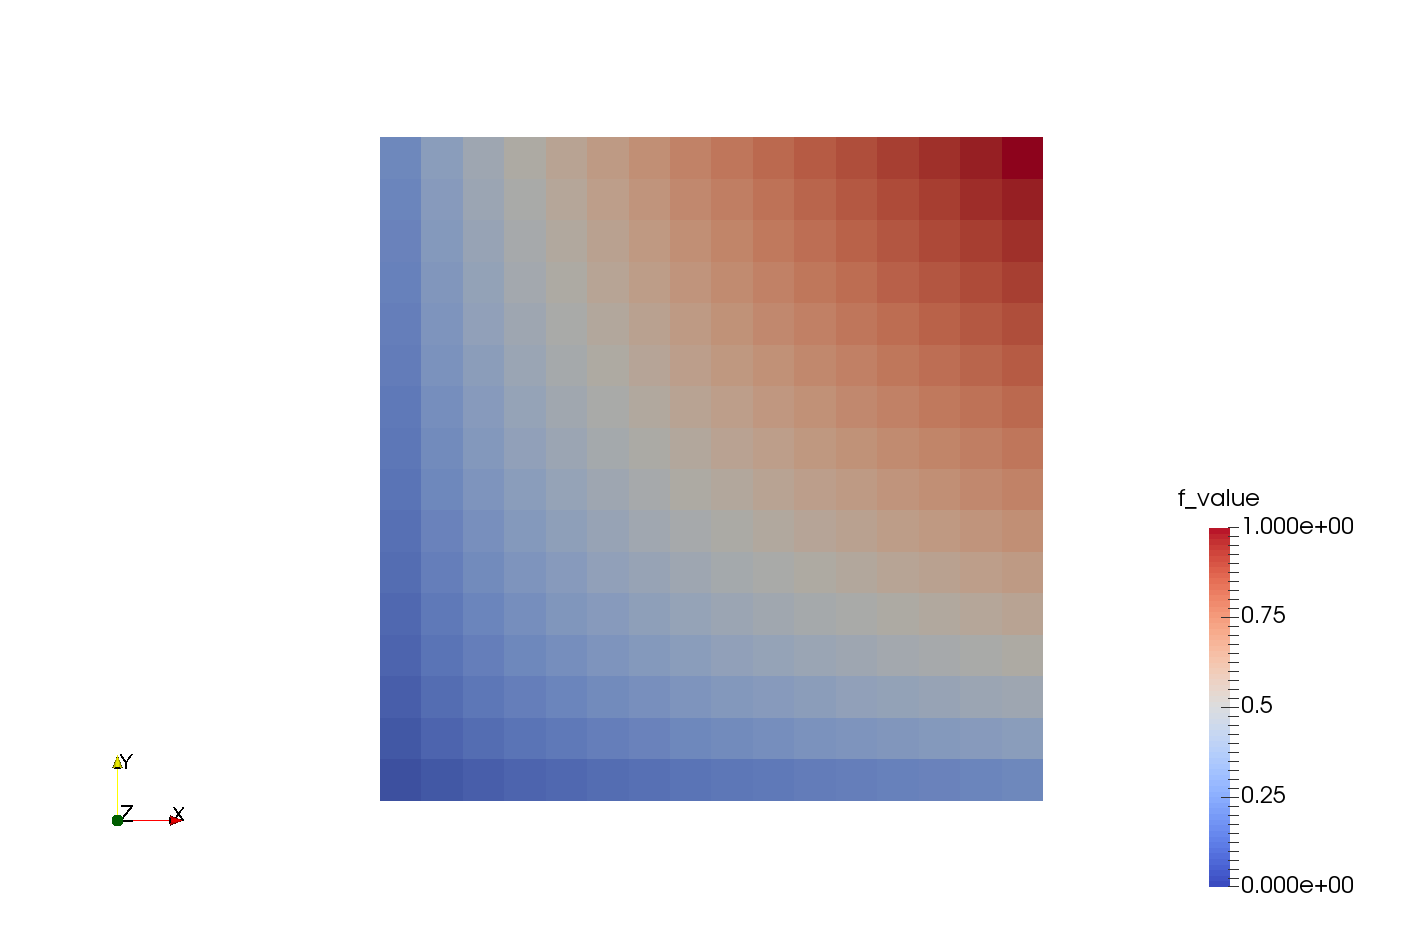
\includegraphics[width =\textwidth]{/results/2/case3-verification-fullgrid.png}
		\centering    
	 \caption{Verification}
	    \label{fig:results2case3Full}	 	 
    \end{subfigure} 
    \caption{(a) Combination and (b) verification for case 3}
    \label{fig:results2case3}
\end{figure}
%2figure case 4 verification difference, combigrid, fullgrid alll together
\begin{figure}[h!]
	\centering
    \begin{subfigure}[b]{0.49\textwidth}
	    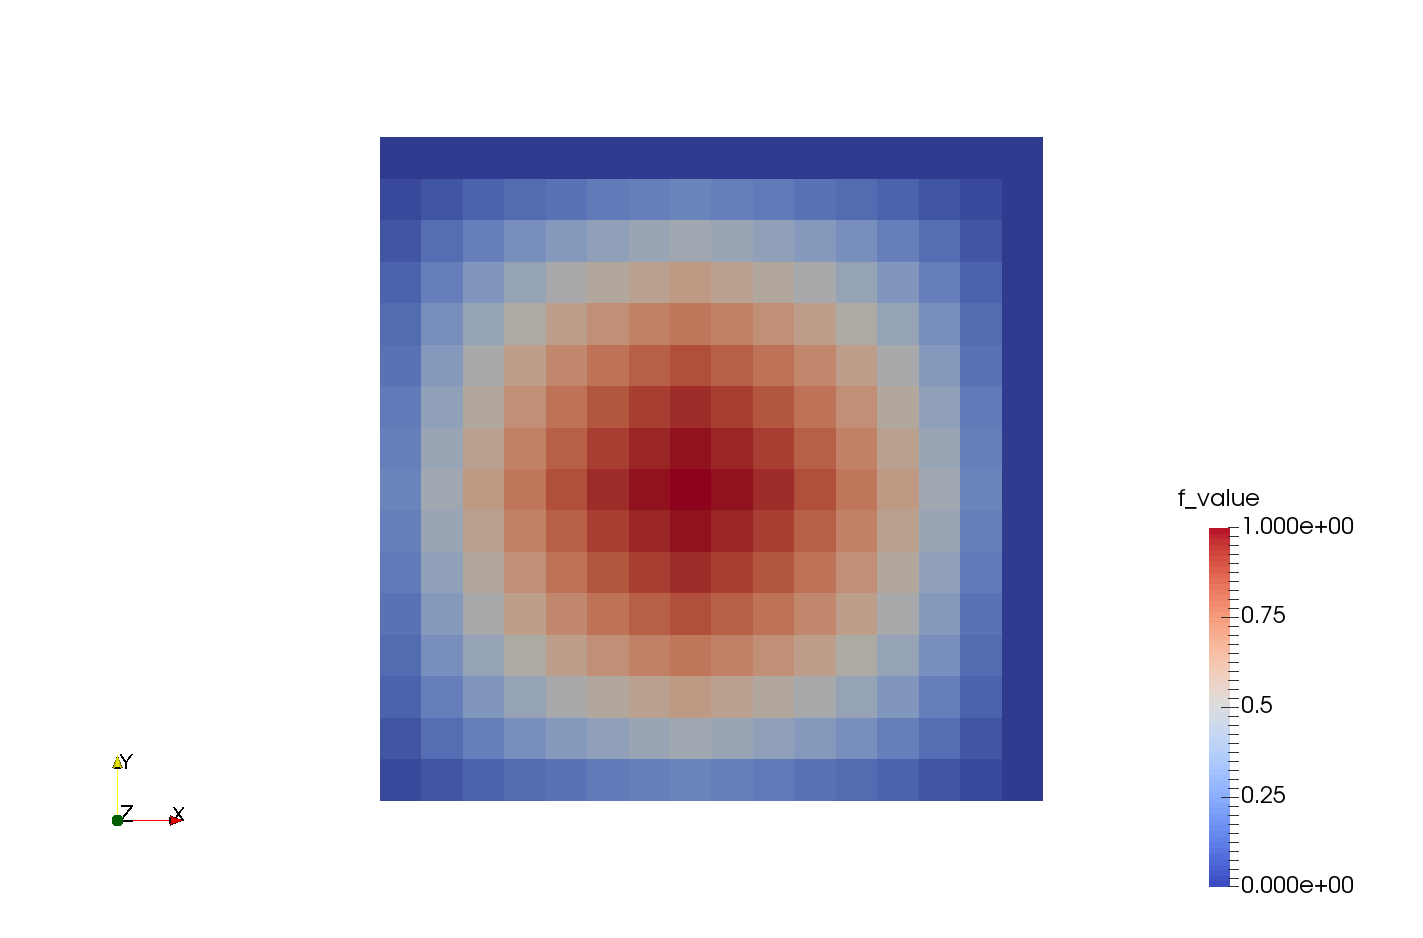
\includegraphics[width =\textwidth]{/results/2/case4-verification-combination.png}
	    %\vspace{3em}
		\centering
        \label{fig:results2case4Combi}
        \caption{Combination}
    \end{subfigure} 
    \begin{subfigure}[b]{0.49\textwidth}    
	    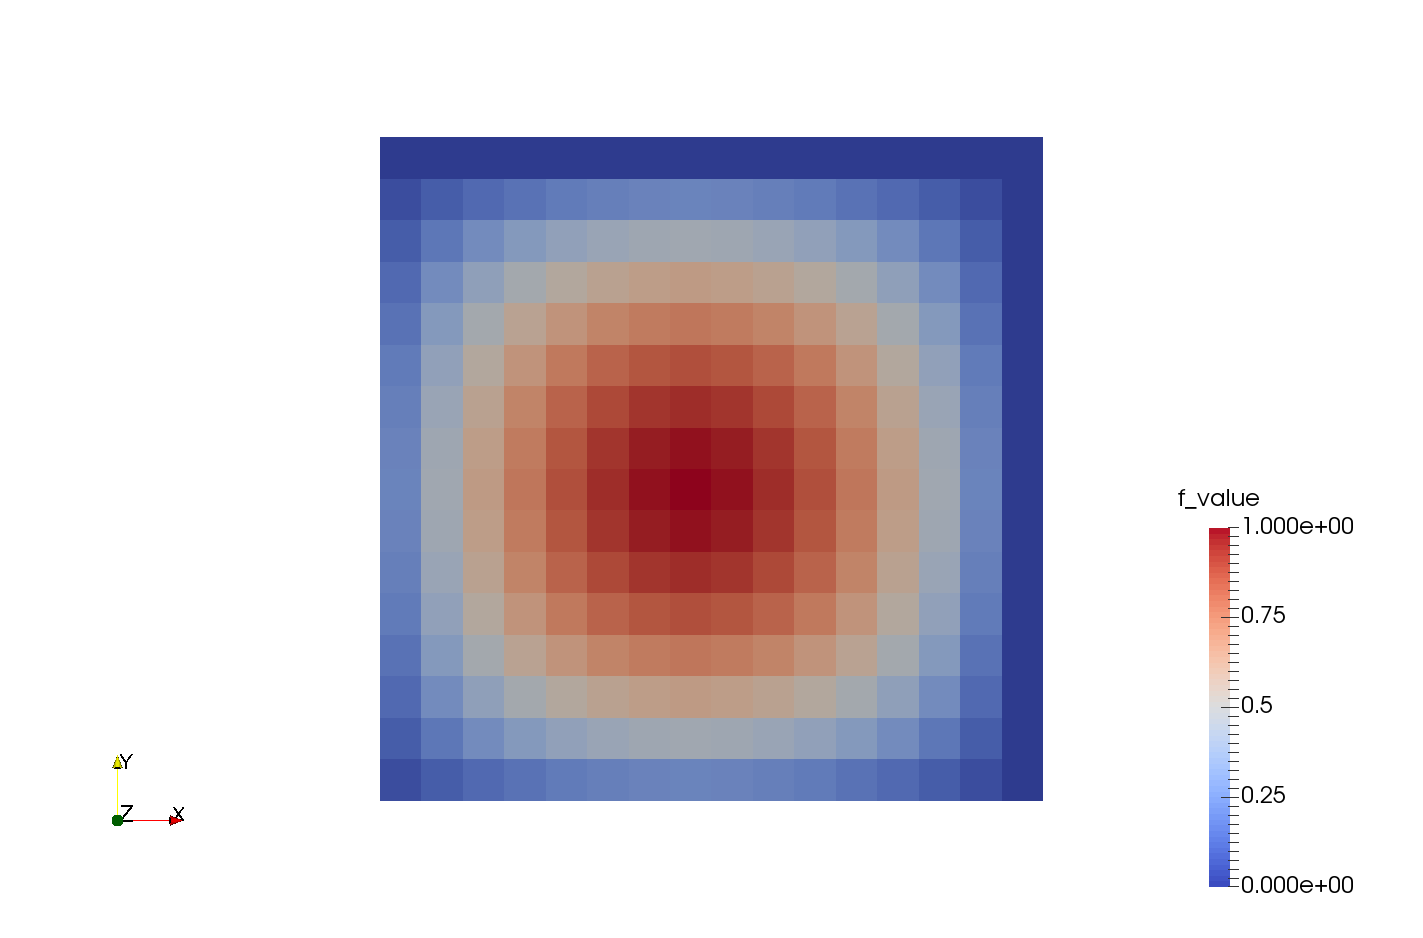
\includegraphics[width =\textwidth]{/results/2/case4-verification-fullgrid.png}
		\centering    
	 \caption{Verification}
	    \label{fig:results2case4Full}	 	 
    \end{subfigure} 
    \caption{(a) Combination and (b) verification for case 4}
    \label{fig:results2case4}
\end{figure}

%Case 1-4 differences
\begin{figure}[h!]
	\centering
    \begin{subfigure}[b]{0.49\textwidth}
	    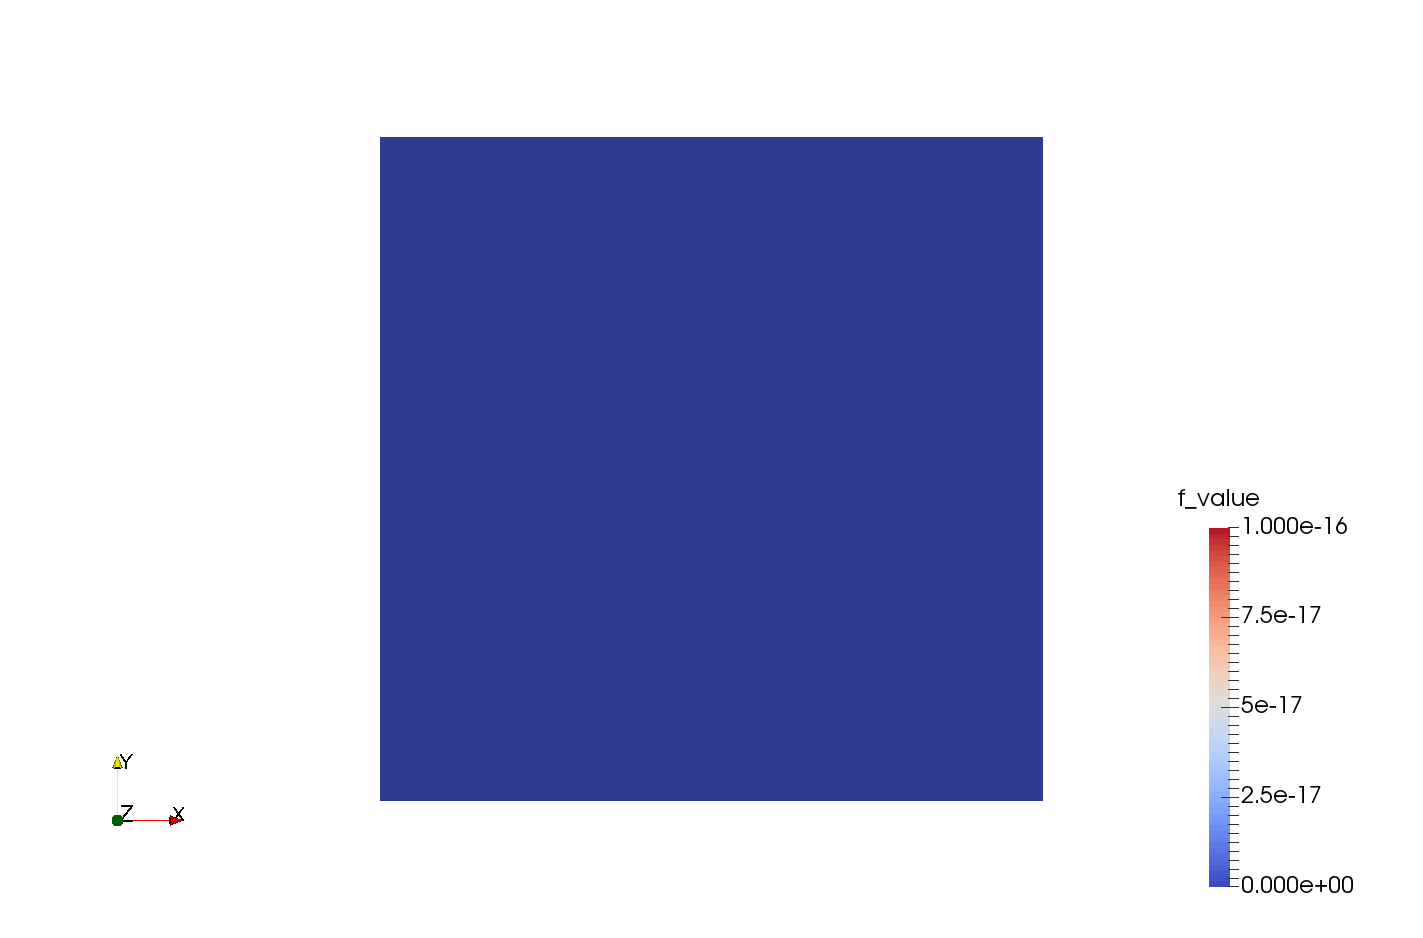
\includegraphics[width =\textwidth]{/results/2/case1-verification-difference.png}
	    %\vspace{3em}
		\centering
        \label{fig:results2case1Diff}
        \caption{Case 1}
    \end{subfigure} 
    \begin{subfigure}[b]{0.49\textwidth}    
	    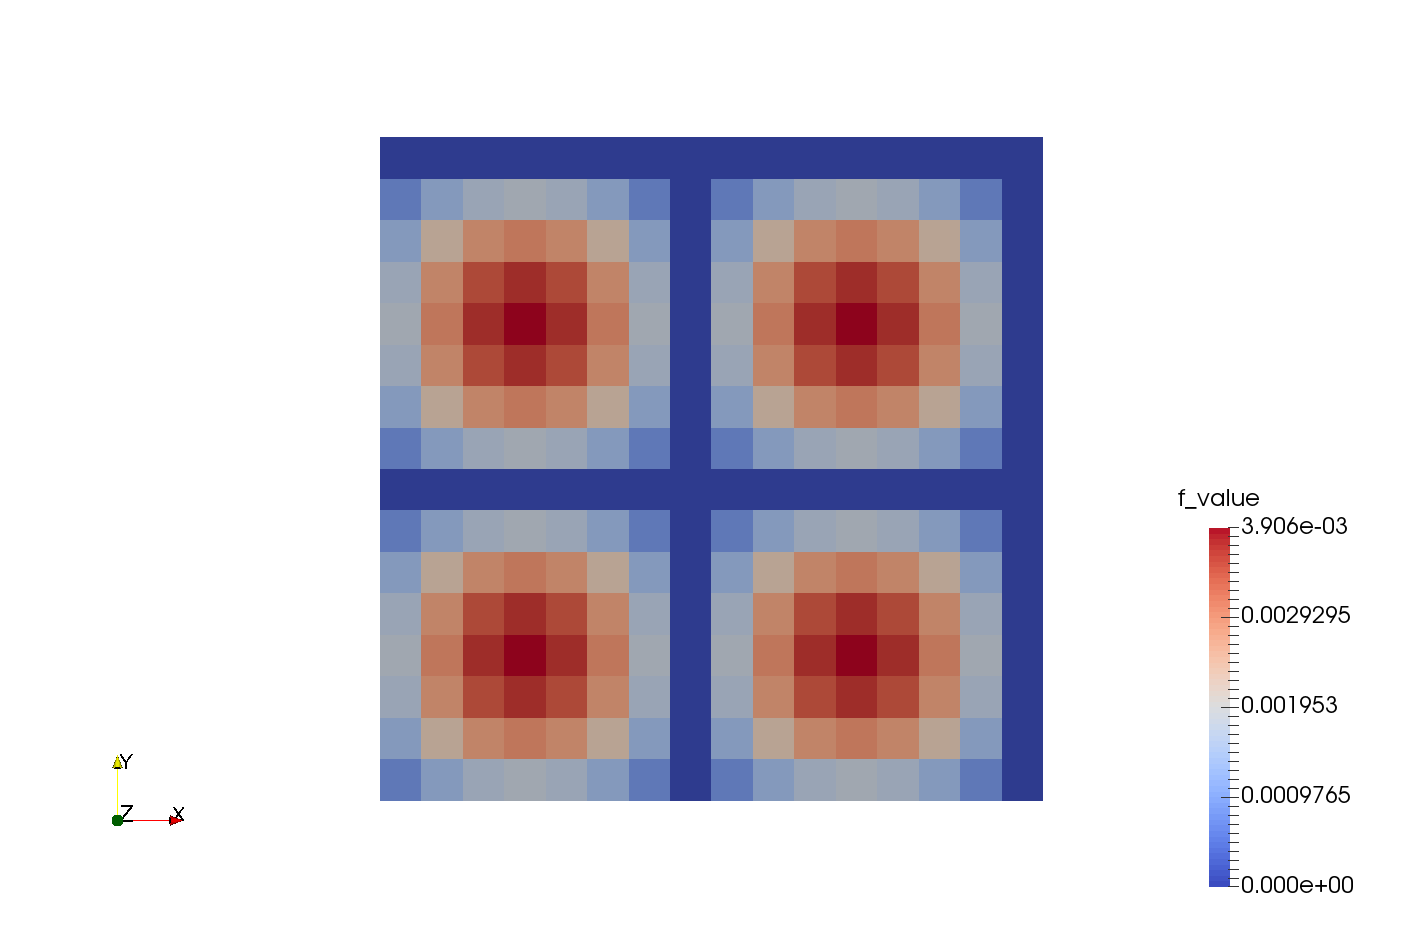
\includegraphics[width =\textwidth]{/results/2/case2-verification-difference.png}
		\centering    
	 \caption{Case 2}
	    \label{fig:results2case2Diff}	 	 
    \end{subfigure} 
    \begin{subfigure}[b]{0.49\textwidth}
	    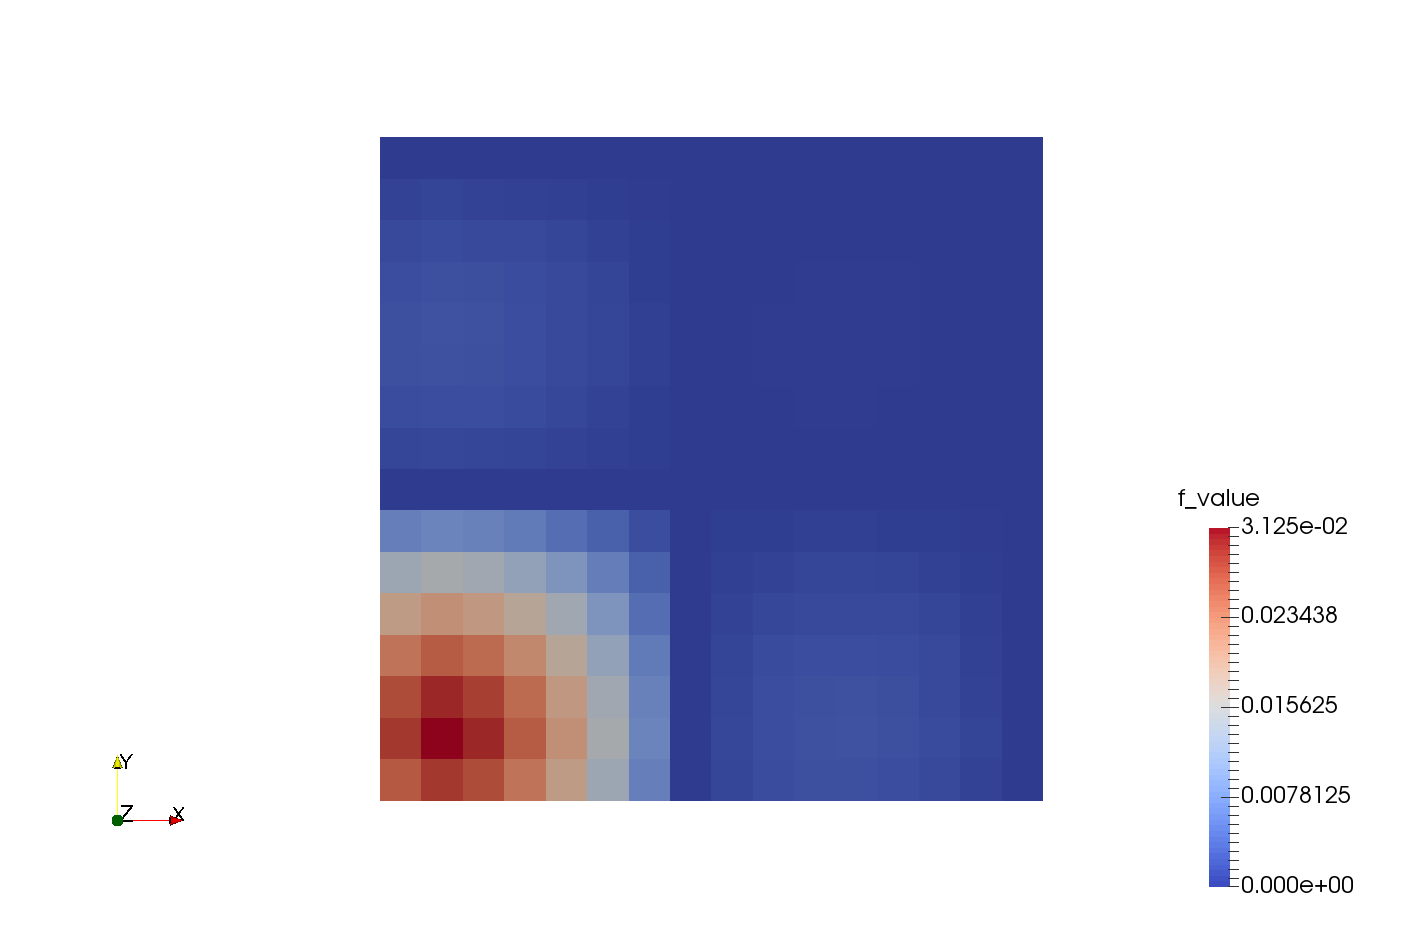
\includegraphics[width =\textwidth]{/results/2/case3-verification-difference.png}
	    %\vspace{3em}
		\centering
        \label{fig:results2case3Diff}
        \caption{Case 3}
    \end{subfigure} 
    \begin{subfigure}[b]{0.49\textwidth}    
	    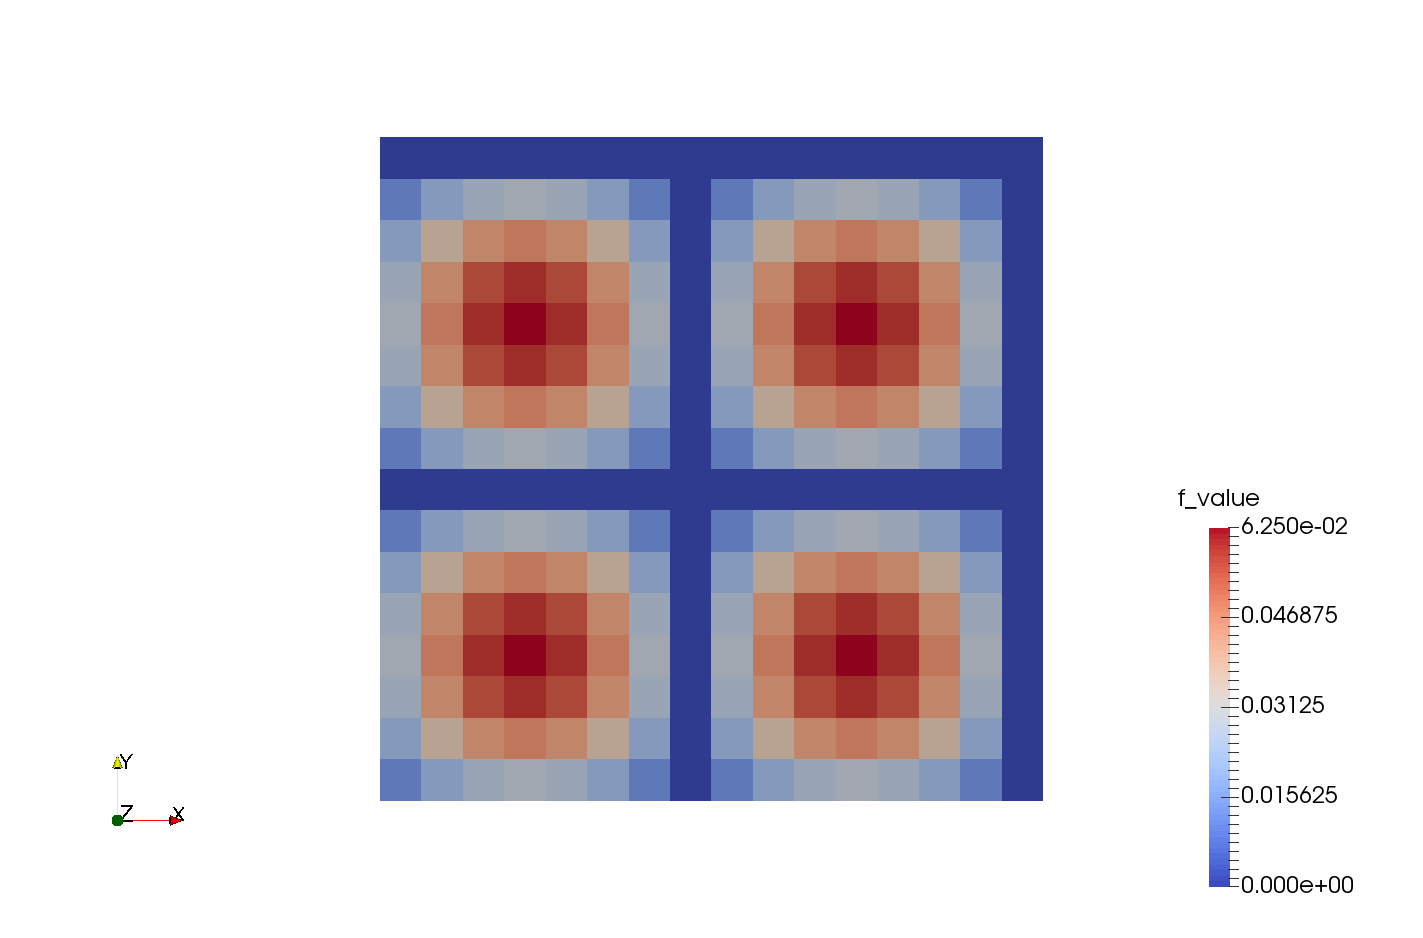
\includegraphics[width =\textwidth]{/results/2/case4-verification-difference.png}
		\centering    
	 \caption{Case 4}
	    \label{fig:results2case4Diff}	 	 
    \end{subfigure} 
    \caption{Difference case 1-4}
    \label{fig:results2case1-4Diff}
\end{figure}


The absolute values of the general error for cases 1 to 4 are compiled in the table \ref{table:GenError}. The general error is 0 for case 1, as already discussed. Case 4 shows a much higher absolute error as the function has a multiplicative factor of 16, leading to higher function values. 

\begin{table}[h]
\centering
\label{table:GenError}
\caption{The resulting general error for cases 1-4 for verification of components}
\vspace{1em}
\begin{tabular}{| c | c | c |}
\hline
 Test Case Number & Function &  General Error\\
 \hline
 1 & $f(x)=x^2+y^2$ & 0 \\
 \hline
 2 & $f(x)=x^2 \cdot y^2 $ & 0.4306\\
 \hline
 3 & $f(x)=\sqrt[2]{x} \cdot \sqrt[2]{y}$ & 0.9224\\
 \hline
 4 & $f(x)=16 \cdot x(1-x)y(1-y)$ & 6.8906 \\
 \hline
\end{tabular}
\end{table}

\section{Results of local refinement (spatial adaptivity)}
Based on the the fact that the current method has been verified, next two different cases are checked for local refinement -- one simply to ensure the proper functionality of the implementation of recursive tree,  and second for the test cases presented above. 

\subsection{Error indicator based on predefined error function}
As explained earlier, the objective here is to come up with a valid test case for local refinement. Based on author's background in mesh generation, there is a technique specially for unstructured grid generation with background predefined function \cite{Henshaw1996} and adaptive grid generation algorithm\cite{Ebeida2010}. Motivated by ideas presented we will enforce a predefined error to the problem by defining an error function which is higher than our threshold for certain regions. This way we can predict the expected working of the local refinement exactly. For better clarity, the solution tree structure is presented in figure \ref{fig:QuadTreeRoot} and the predefined function with it's image on the unit square problem is presented in figure \ref{fig:Predef}.\\

% 3figure of tree from aastha
% 3figure of predefined error from aastha

\begin{figure}[h]
	\centering
	    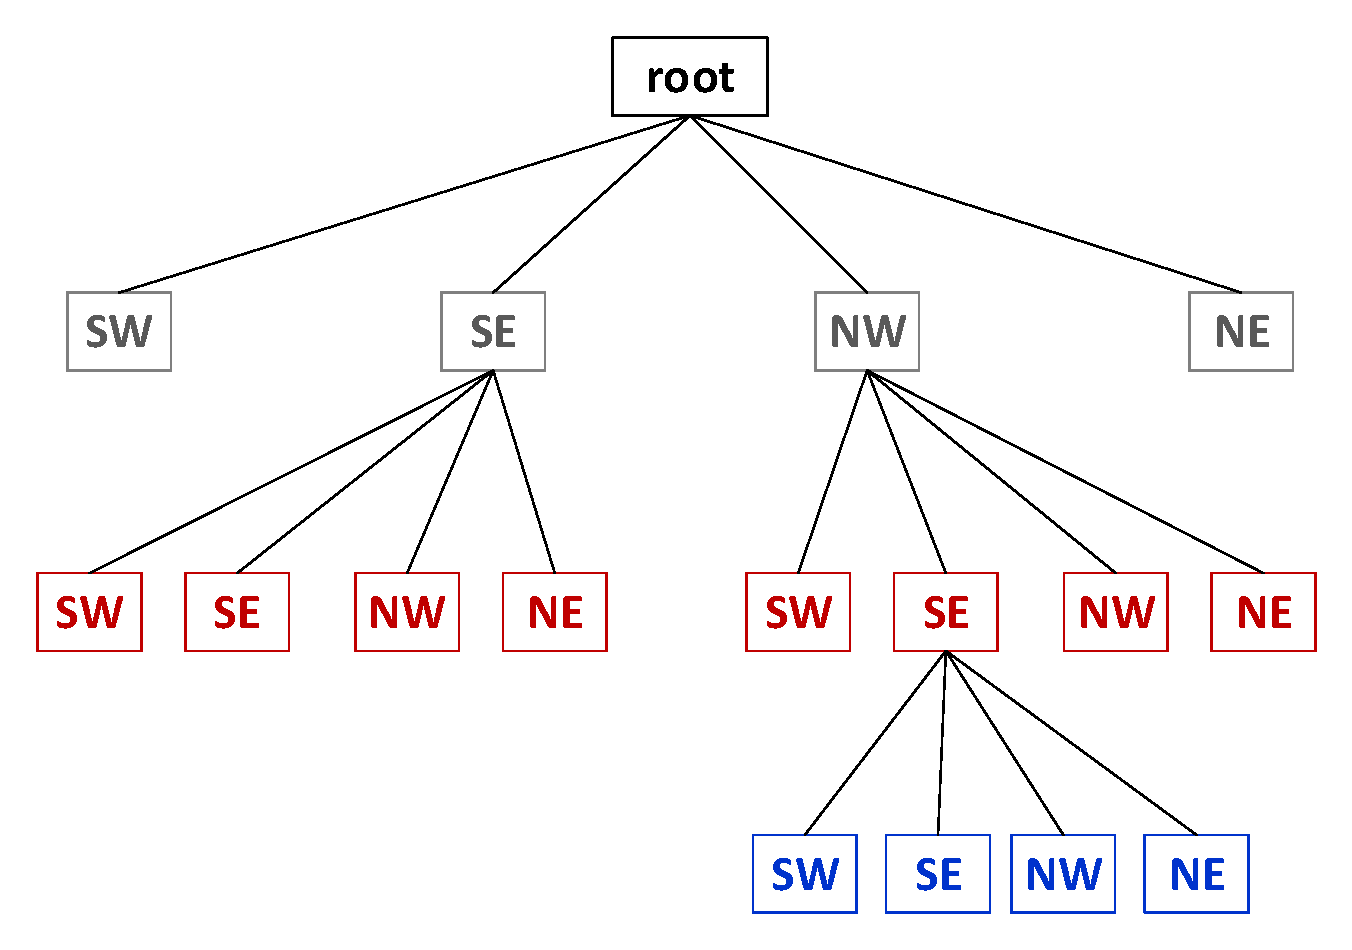
\includegraphics[width =0.66\textwidth]{/results/3/QuadTreeRoot.pdf}
	    %\vspace{3em}
		\centering
        \caption{Quad tree representation}
        \label{fig:QuadTreeRoot}
\end{figure}


		
\begin{figure}[h]
	\centering
    \begin{subfigure}[b]{0.66\textwidth}    
	    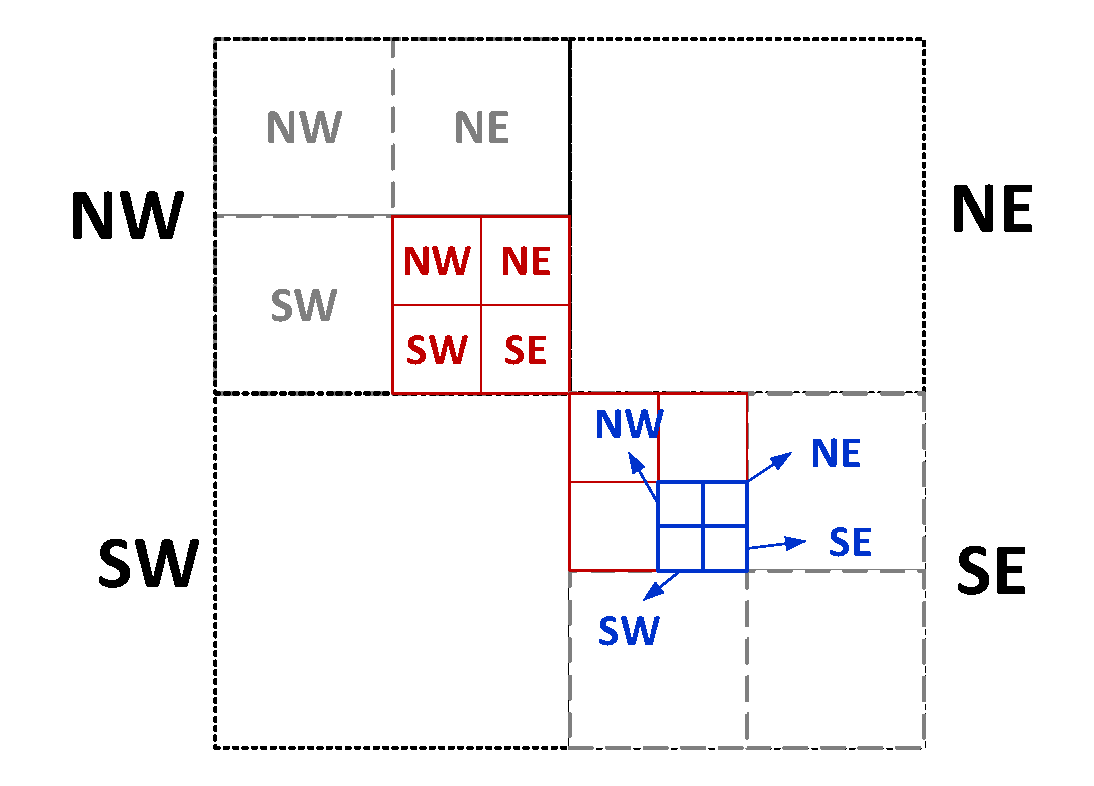
\includegraphics[width =\textwidth]{/results/3/QuadTreeSquare.pdf}
		\centering    
		\caption{Quad tree}
		\label{fig:QuadTreeSquare}
    \end{subfigure} 
    \begin{subfigure}[b]{0.75\textwidth}
	    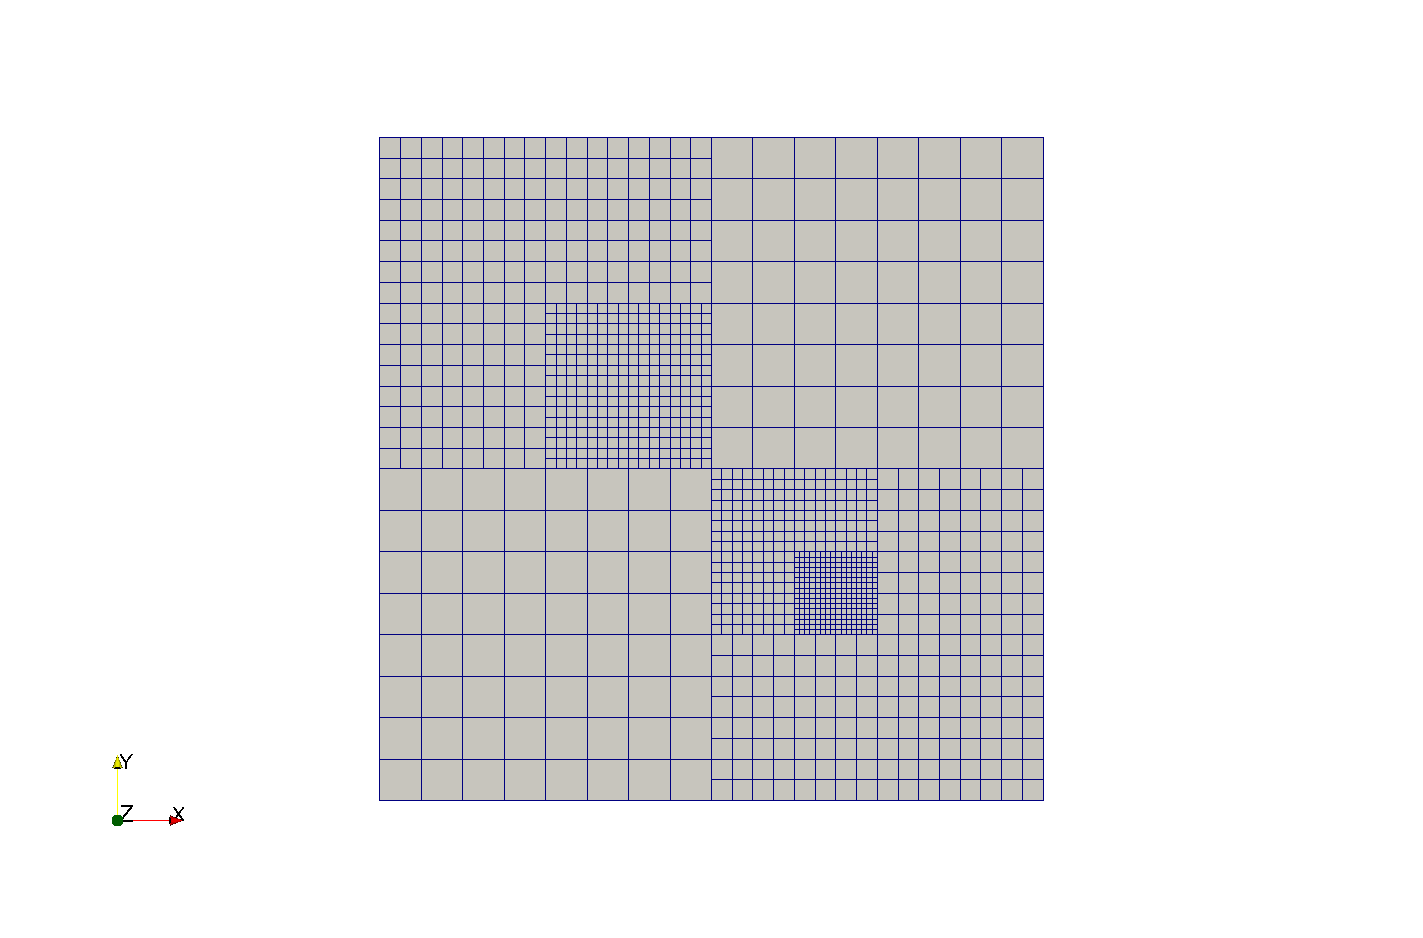
\includegraphics[width =\textwidth]{/results/3/predefined-refinement-vtk.png}
	    %\vspace{3em}
		\centering
        \caption{Predefined refinement}
        \label{fig:PredefRefine}
    \end{subfigure} 
    \caption{Predefined}
    \label{fig:Predef}
\end{figure}

% 3figure predefined refinement from VTK
% 3figure predefined error from VTK

		
\begin{figure}[h]
	\centering
	    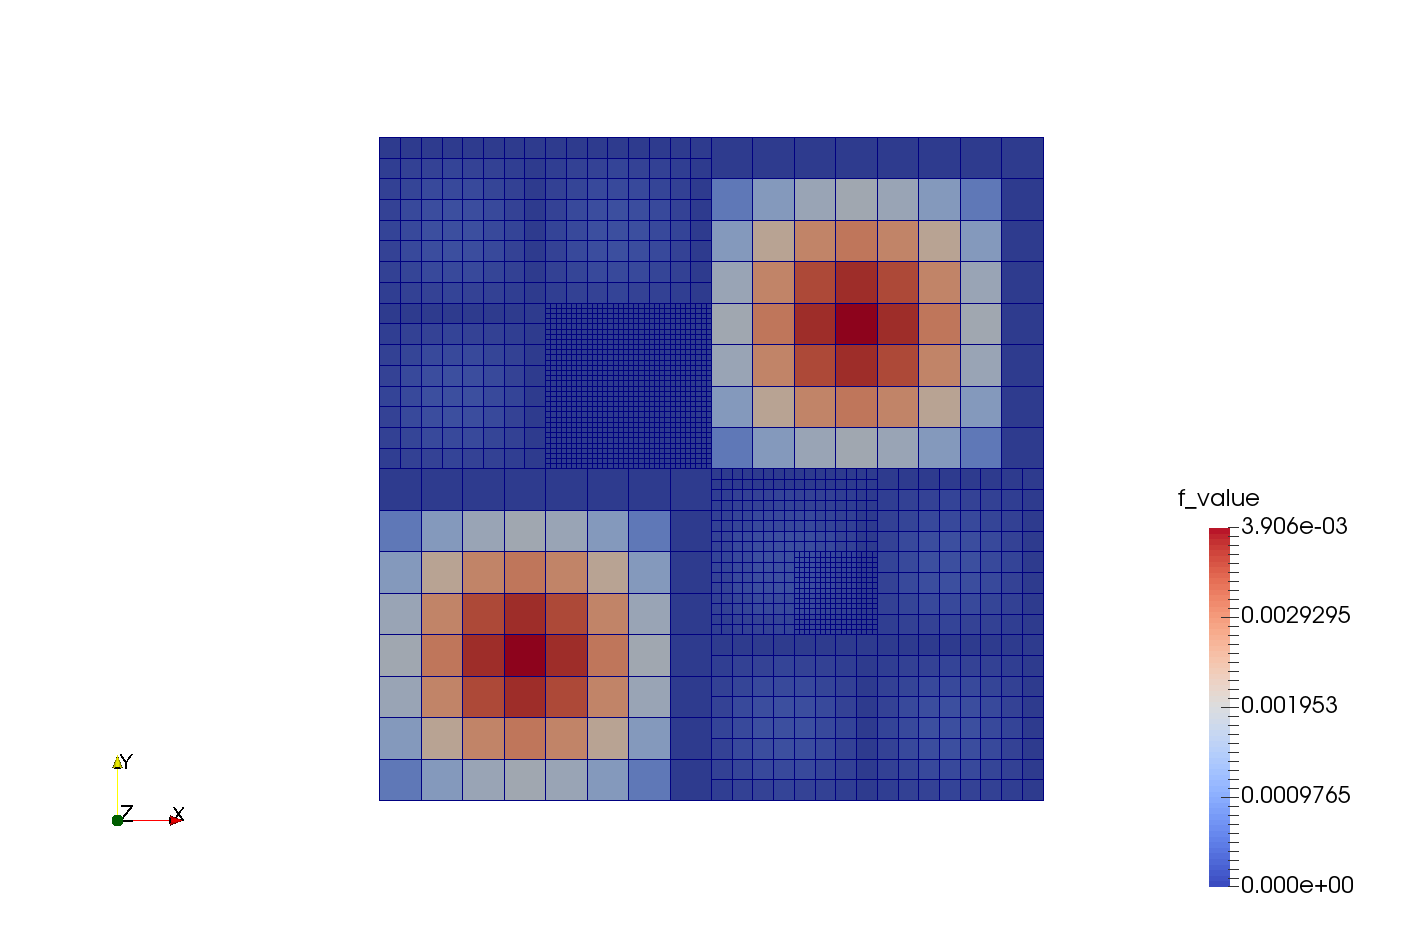
\includegraphics[width =0.75\textwidth]{/results/3/predefined-error-vtk.png}
		\centering    
	 \caption{Predefined error}
       \label{fig:PredefError}
\end{figure}

As seen in figure \ref{fig:PredefError}, the solution to this case matches the expectations. Based on this result, the final evaluation is performed in the next section.

\subsection{Error indicator based on solution of combination technique}
After verification of the code in both adaptive and non-adaptive cases, the next focus is on further investigation into the actual problem at hand, which is performing the adaptation in correspondence with the local error of solution in each node or subtree. For that, an error indicator has been introduced which compares the solution to the full grid method. The primary reason for defining some extra test cases in the verification part was that to be able to observe how the local refinement works with different cases, otherwise there is much similarity between case 2, 3 and 4. The results are visualized in figures \ref{fig:AdaptiveCase2}, \ref{fig:AdaptiveCase3} and \ref{fig:AdaptiveCase4} for cases 2,3 and 4, respectively. \\


%4adaptive case 2: before refinement and after refinement together 
\begin{figure}[h]
	\centering
    \begin{subfigure}[b]{0.49\textwidth}
	    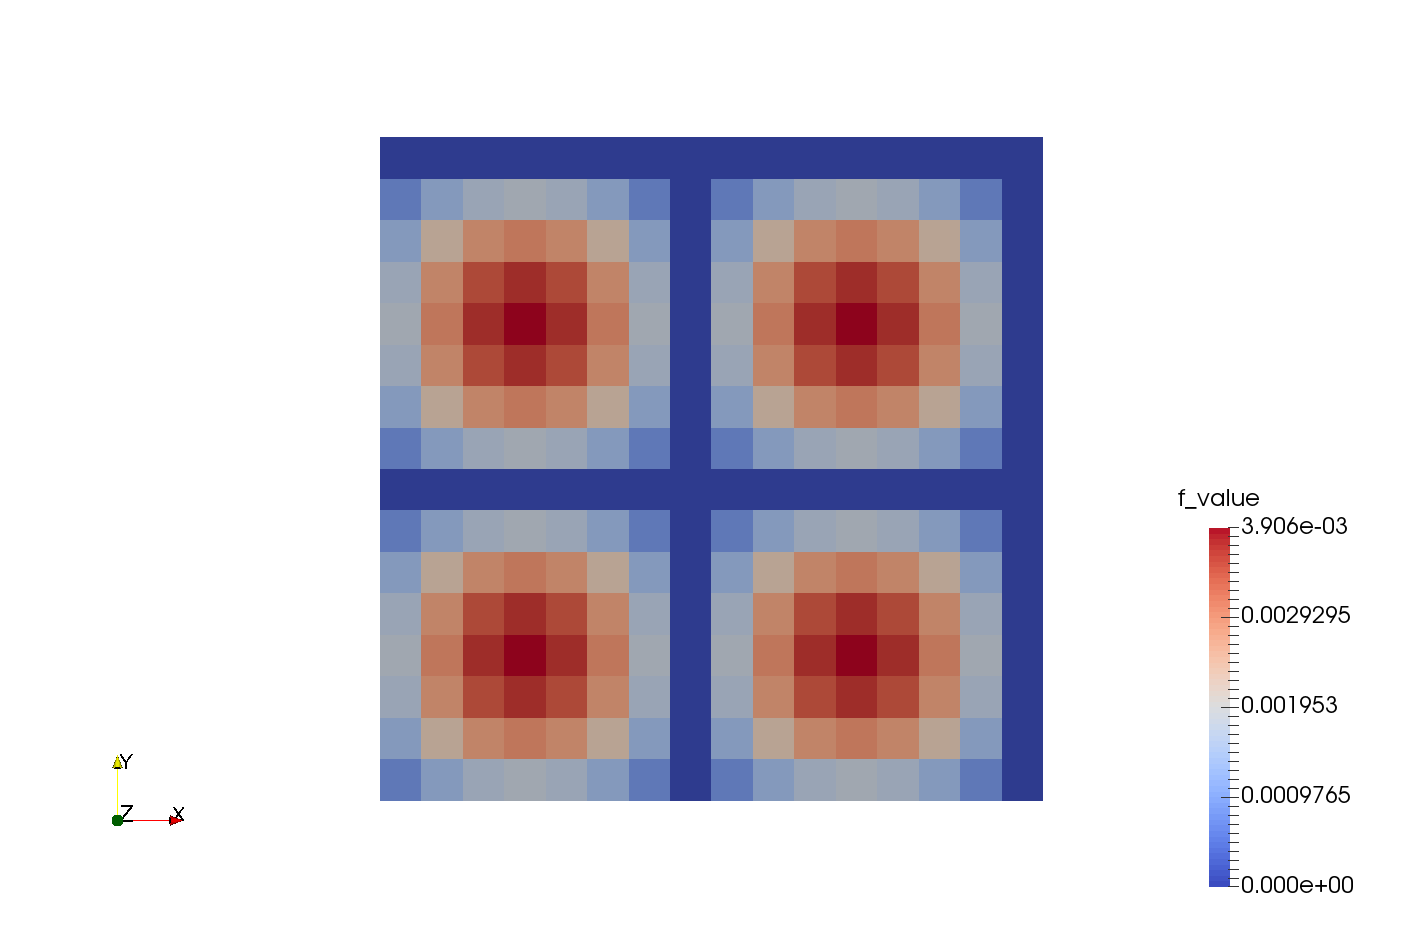
\includegraphics[width =\textwidth]{/results/4/case2-adaptive-before-refinement.png}
	    %\vspace{3em}
		\centering
        \caption{case 2 before refinement}
        \label{fig:AdaptiveCase2Before}
    \end{subfigure} 
    \begin{subfigure}[b]{0.49\textwidth}    
	    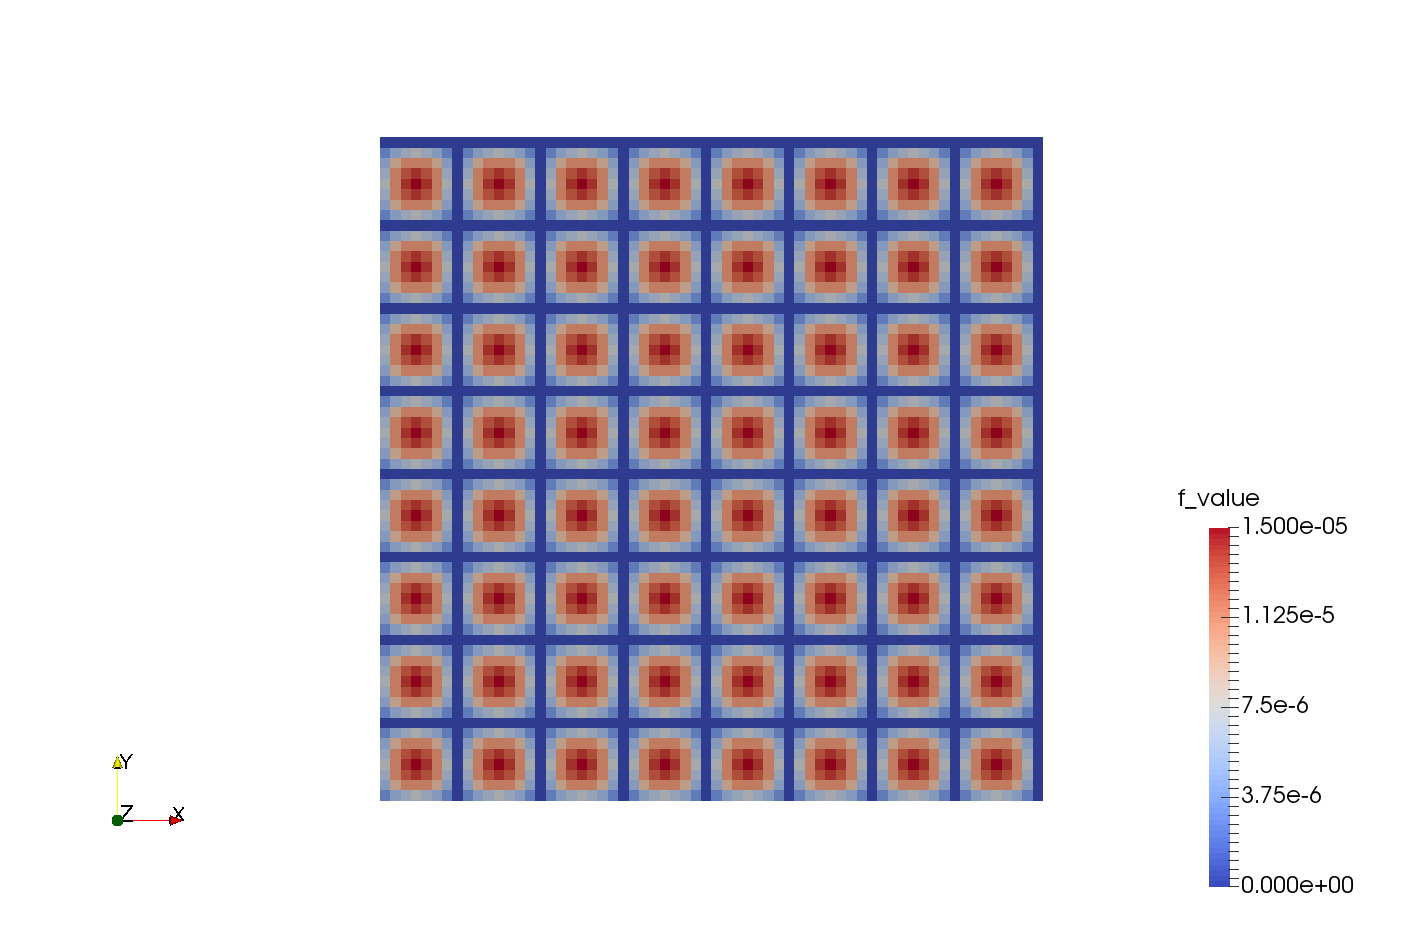
\includegraphics[width =\textwidth]{/results/4/case2-adaptive-after-refinement.png}
		\centering    
	 \caption{case 2 after refinement}
       \label{fig:AdaptiveCase2After}
    \end{subfigure} 
    \caption{Case 2 before and after refinement}
    \label{fig:AdaptiveCase2}
\end{figure}

%4adaptive case 3: before refinement and after refinement together
\begin{figure}[h]
	\centering
    \begin{subfigure}[b]{0.49\textwidth}
	    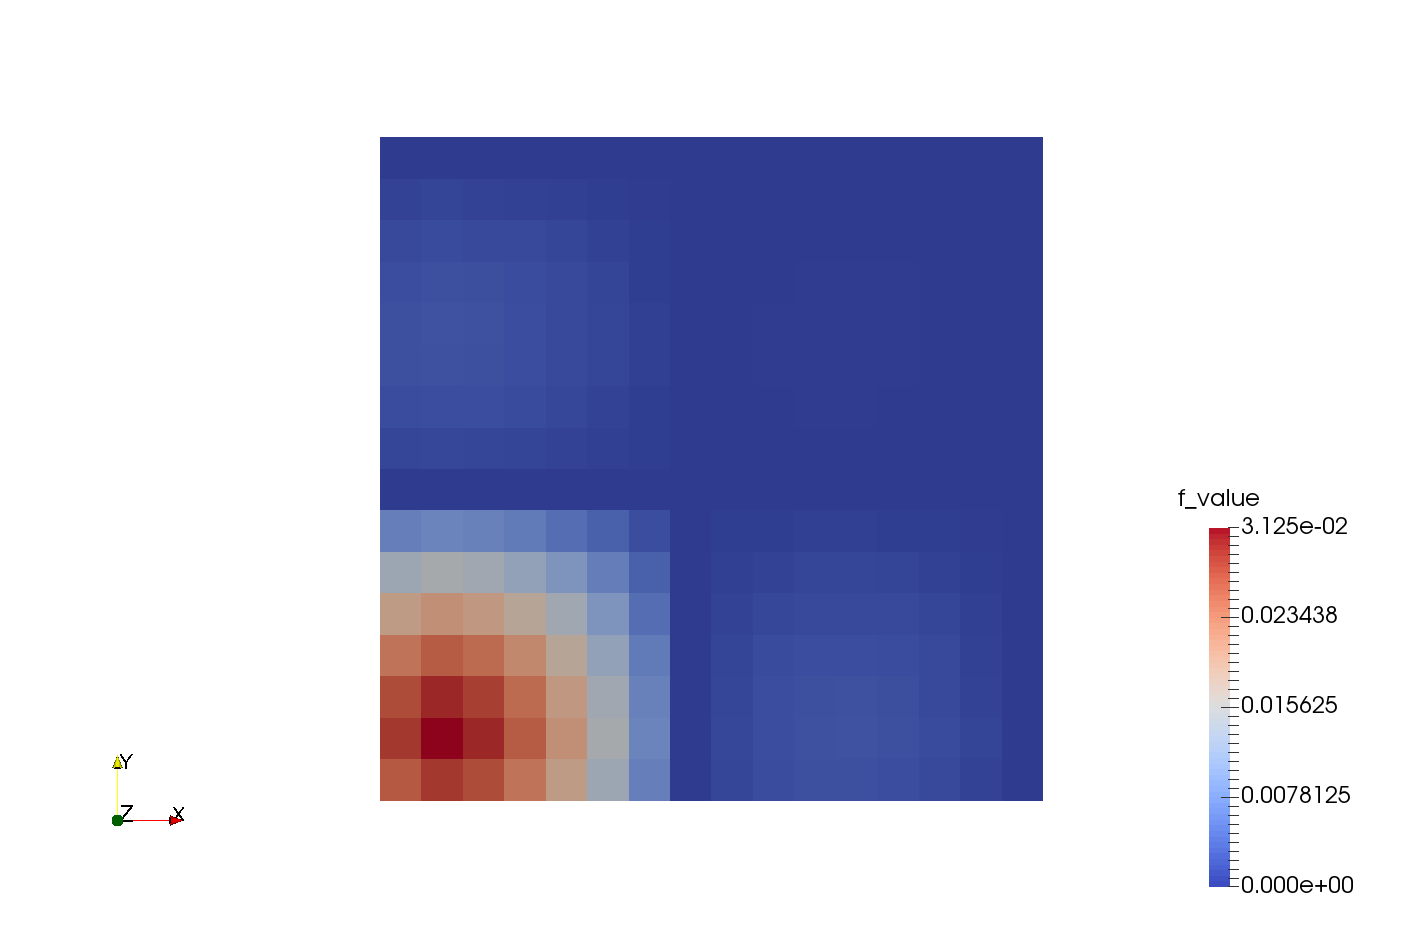
\includegraphics[width =\textwidth]{/results/4/case3-adaptive-before-refinement.png}
	    %\vspace{3em}
		\centering
        \caption{case 3 before refinement}
        \label{fig:AdaptiveCase3Before}
    \end{subfigure} 
    \begin{subfigure}[b]{0.49\textwidth}    
	    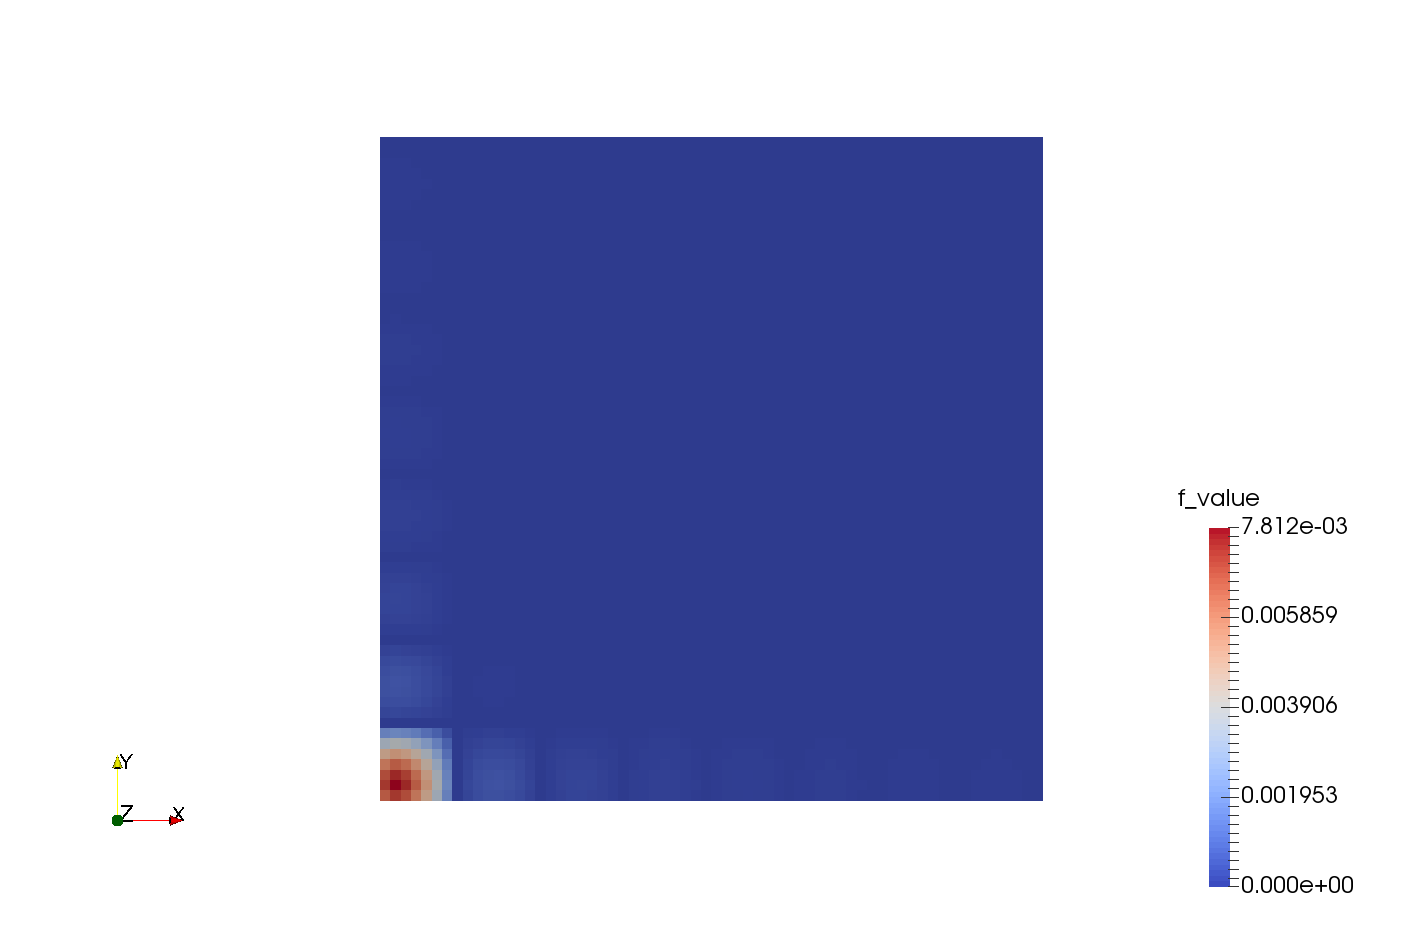
\includegraphics[width =\textwidth]{/results/4/case3-adaptive-after-refinement.png}
		\centering    
	 \caption{case 3 after refinement}
       \label{fig:AdaptiveCase3After}
    \end{subfigure} 
    \caption{Case 3 before and after refinement}
    \label{fig:AdaptiveCase3}
\end{figure}

%4adaptive case 4: before refinement and after refinement together
\begin{figure}[h]
	\centering
    \begin{subfigure}[b]{0.49\textwidth}
	    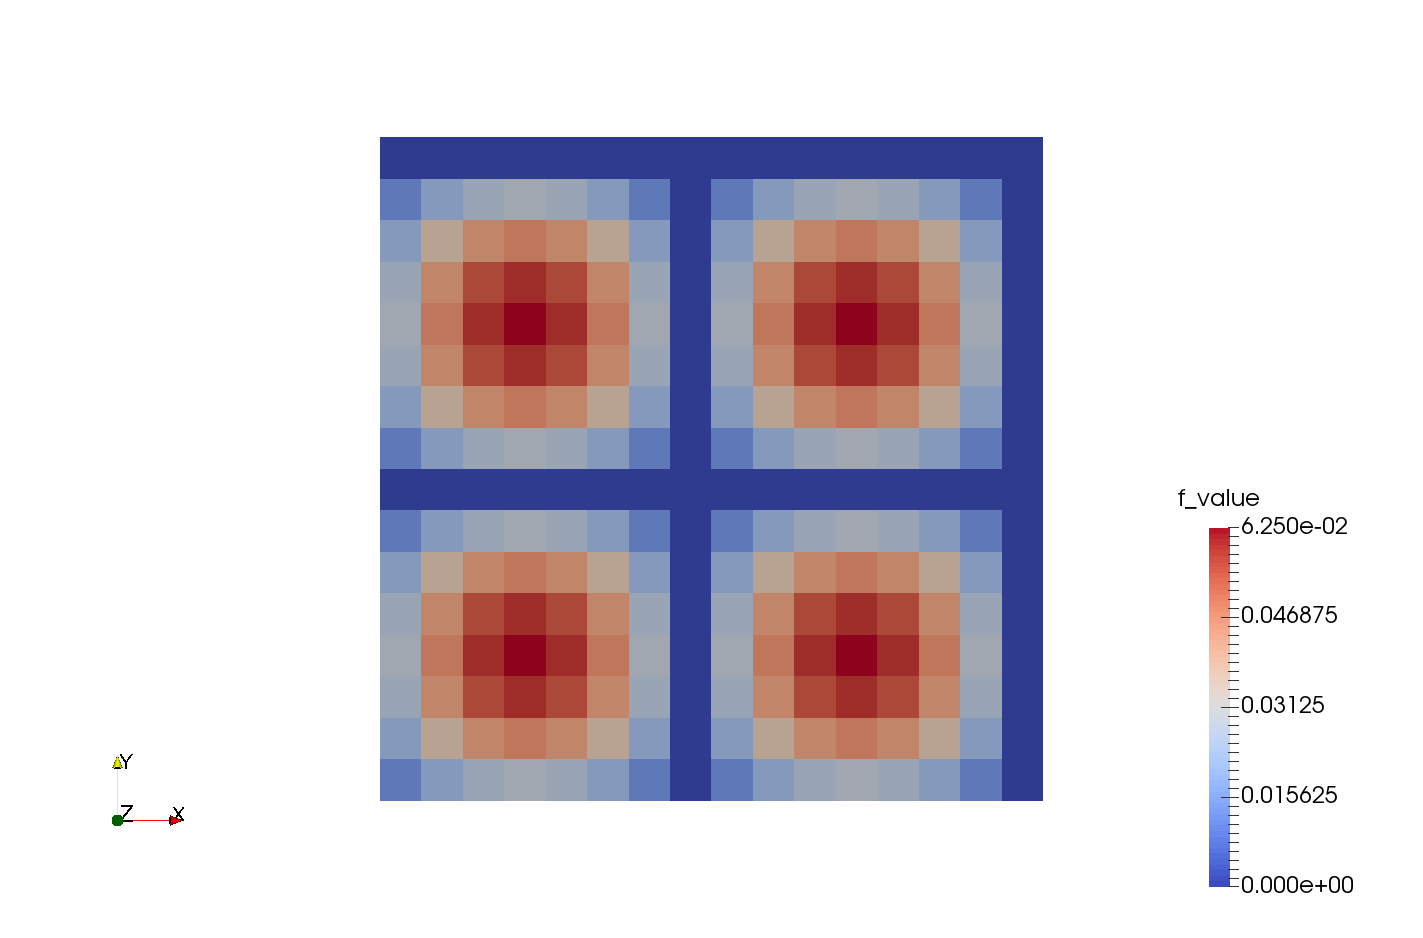
\includegraphics[width =\textwidth]{/results/4/case4-adaptive-before-refinement.png}
	    %\vspace{3em}
		\centering
        \caption{case 4 before refinement}
        \label{fig:AdaptiveCase4Before}
    \end{subfigure} 
    \begin{subfigure}[b]{0.49\textwidth}    
	    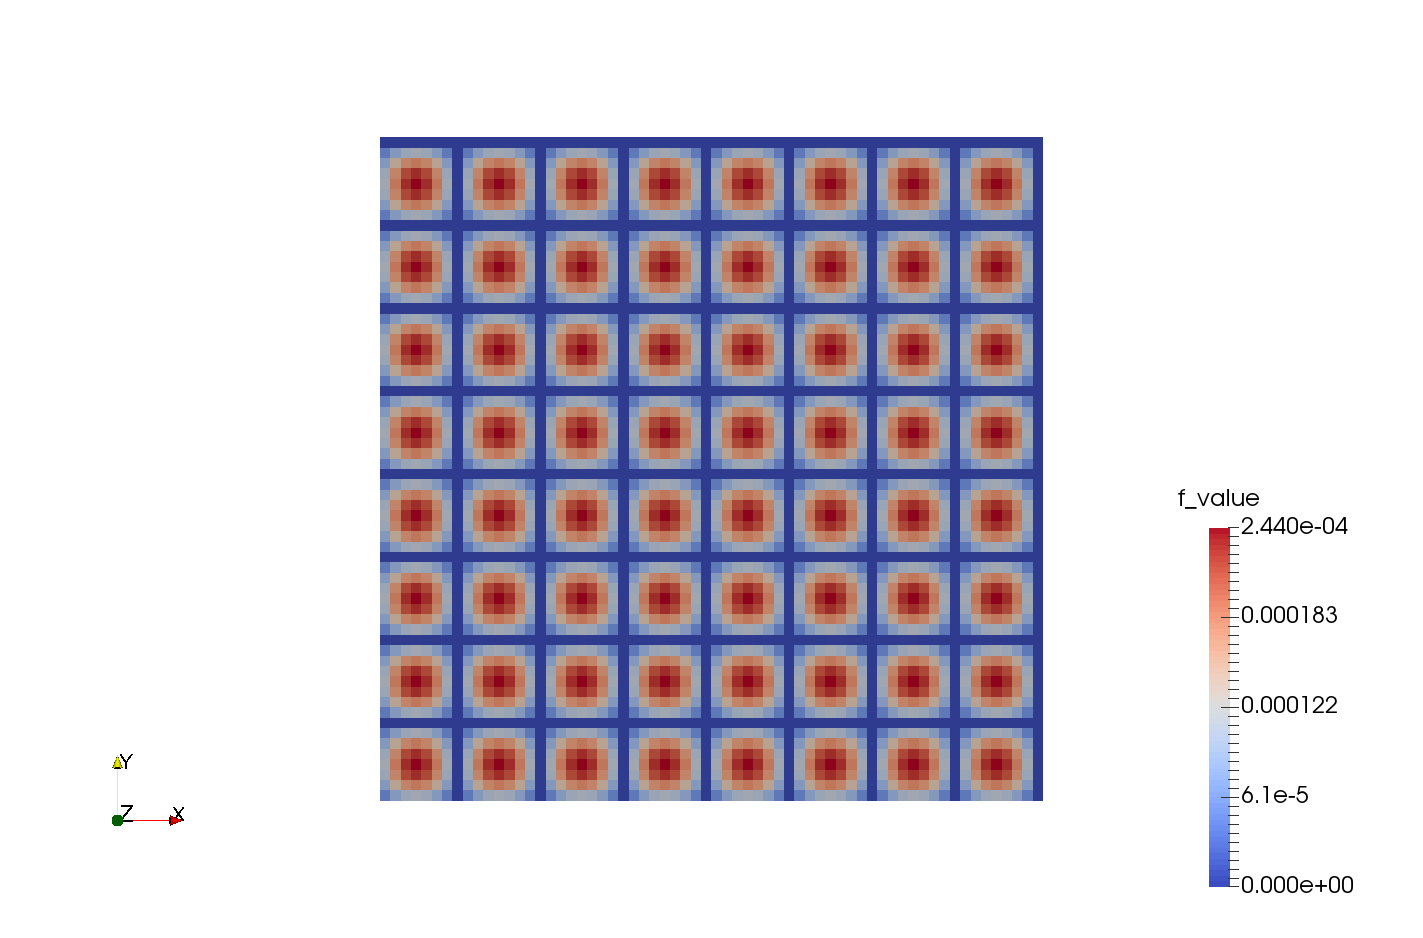
\includegraphics[width =\textwidth]{/results/4/case4-adaptive-after-refinement.png}
		\centering    
	 \caption{case 4 after refinement}
       \label{fig:AdaptiveCase4After}
    \end{subfigure} 
    \caption{Case 4 before and after refinement}
    \label{fig:AdaptiveCase4}
\end{figure}


It is important to point out the necessity of visualizing the error in the solution because from the solution images, the difference is hard to distinguish with human eye.

\section{Error and Accuracy}
In the last section the error is visualized in unit square simply because it doesn't make sense to just give one total error value for a special schemes. The difference here is to have multiple refinement levels performed in a loop/recursive way and then check how the total error acts. Based on arguments in literature a logarithmic behavior is expected. Key factors in the implemented code which are at play are threshold for the error and the level of refinement. Based on them some other schemes imagined here are as follow:
\begin{enumerate}
\item Threshold independent, refinement level changing.
\item Threshold changing, refinement level constant.
\end{enumerate}
The reason for these two scheme is that the results should be separated and based on the factors at play. Figures \ref{fig:ErrorRefinementLevel} and \ref{fig:ErrorThreshod} show the resulting error graphs for cases 2 to 4.

%5figure error threshold independent
%5figure refinement level constant

\begin{figure}[h]
	\centering
	    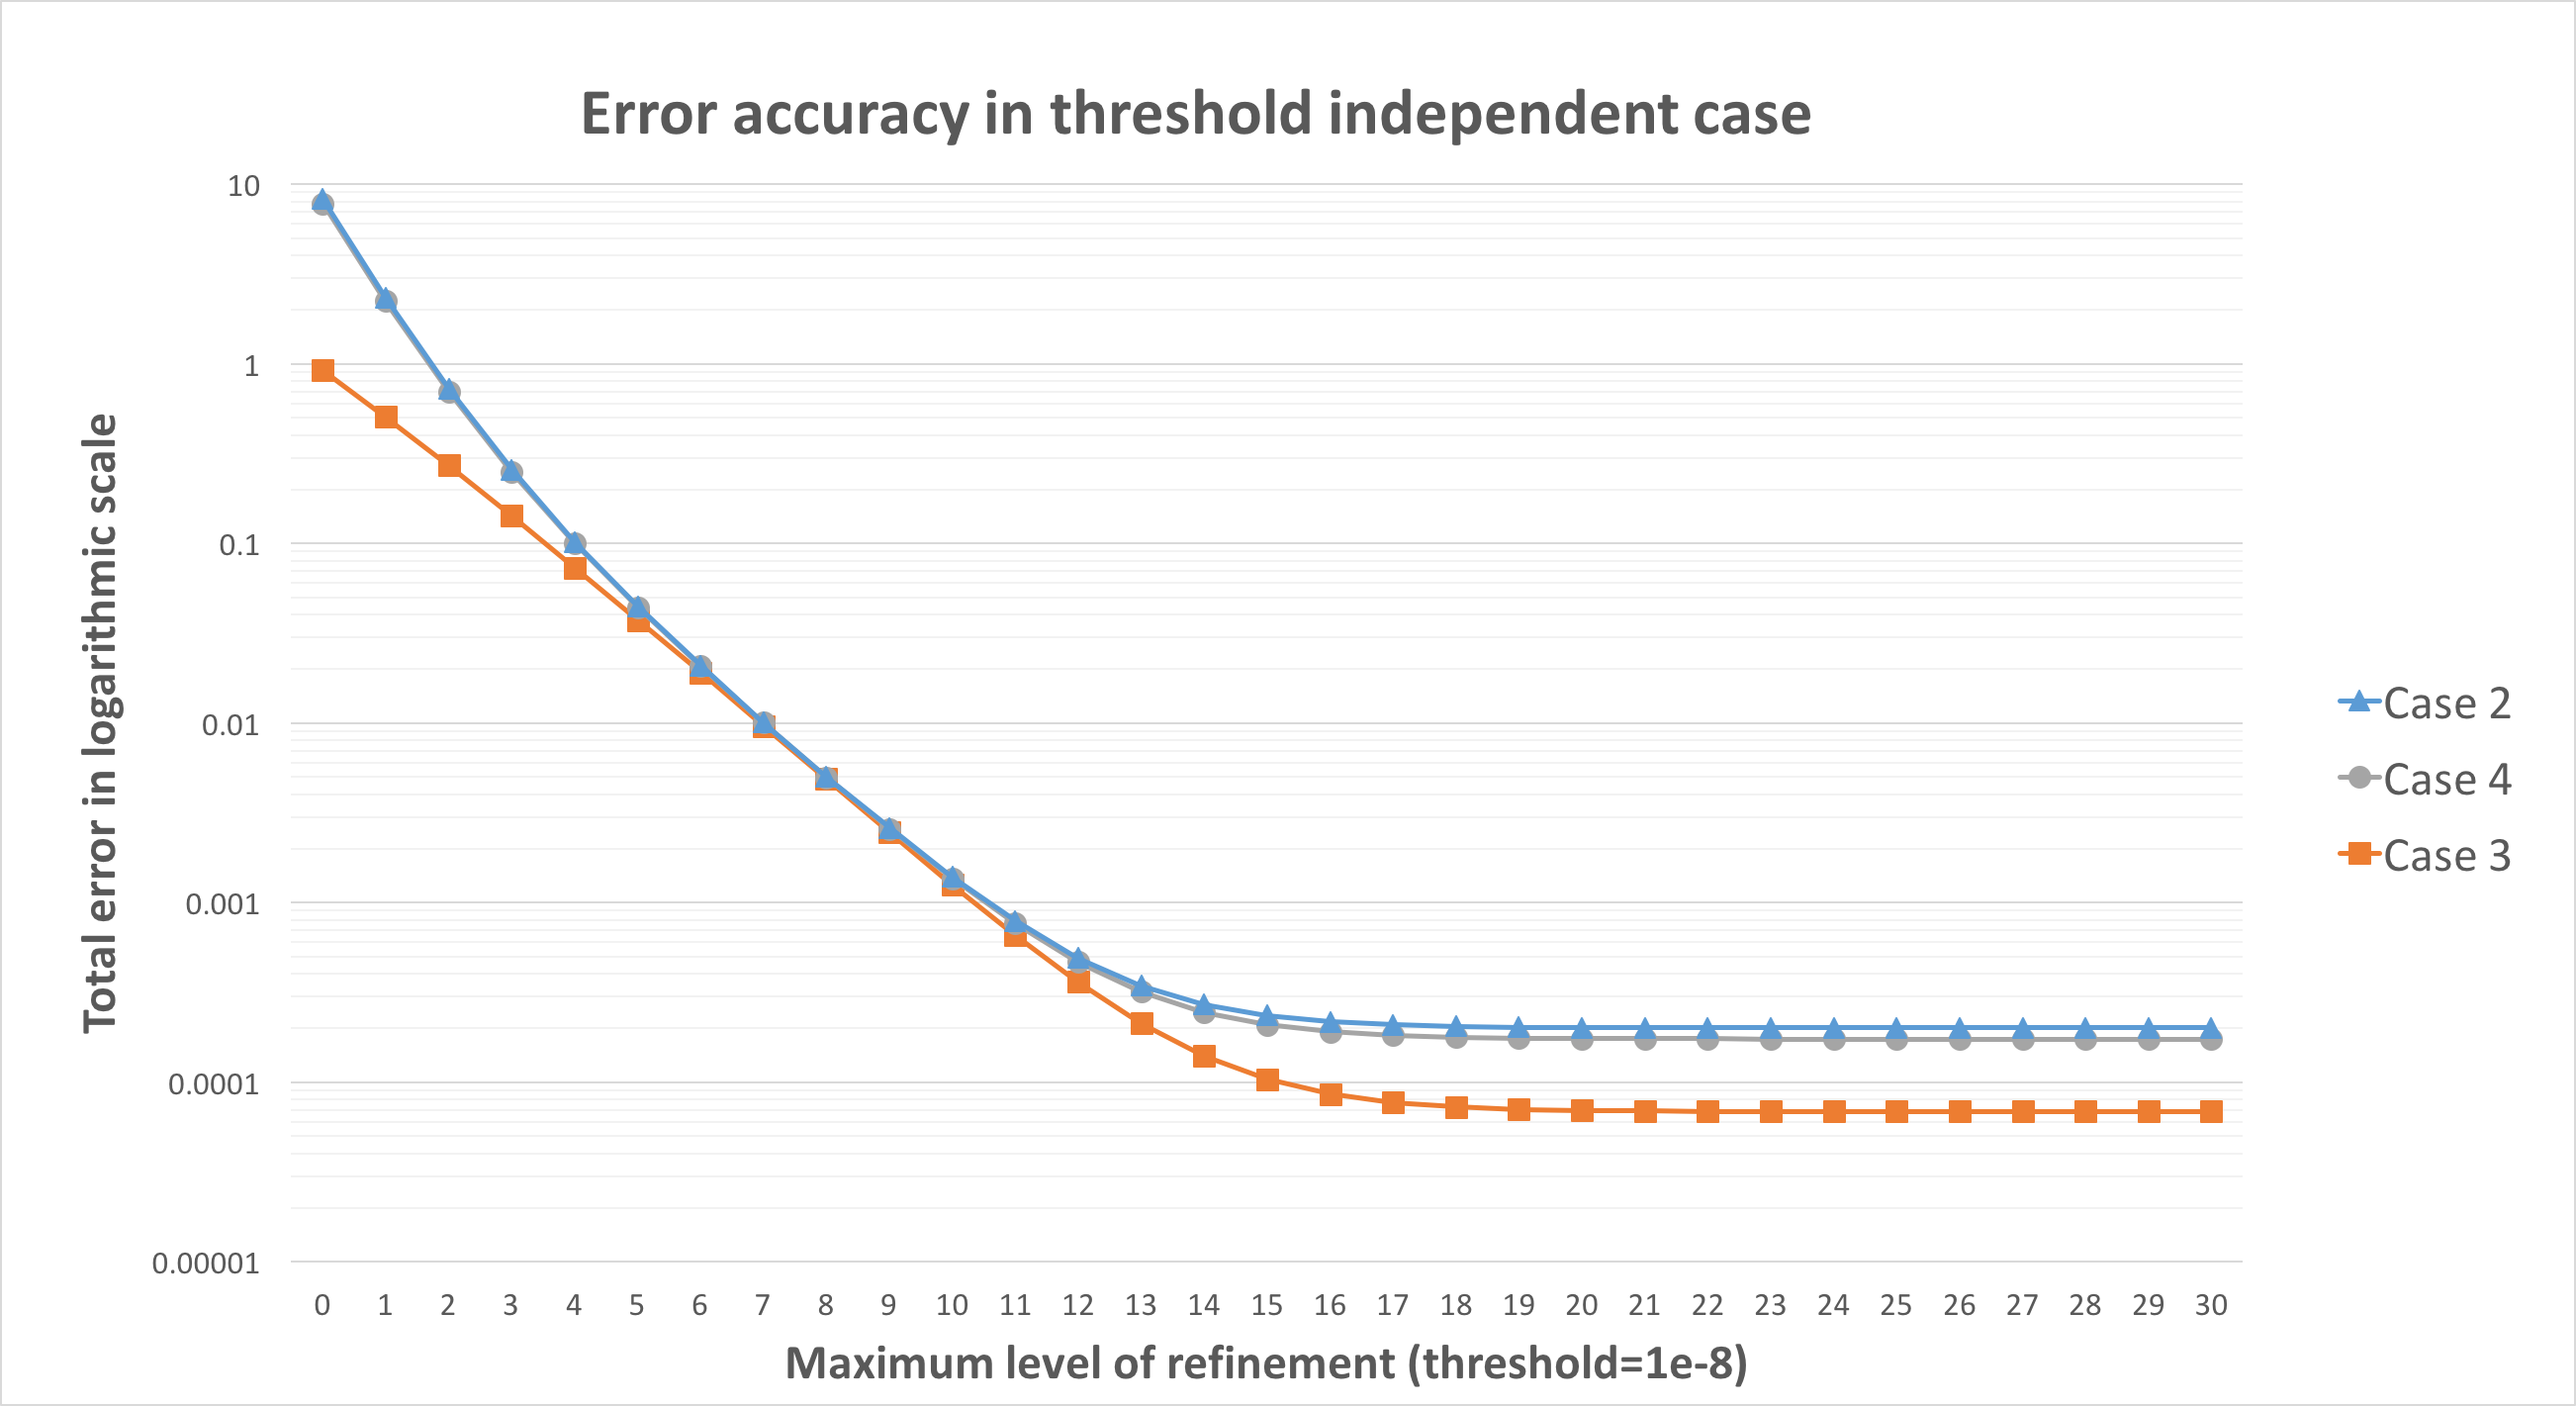
\includegraphics[width =\textwidth]{/results/5/Error-RefinementLevel.png}
		\centering    
	 \caption{Error-RefinementLevel}
       \label{fig:ErrorRefinementLevel}
\end{figure}

\begin{figure}[h]
	\centering
	    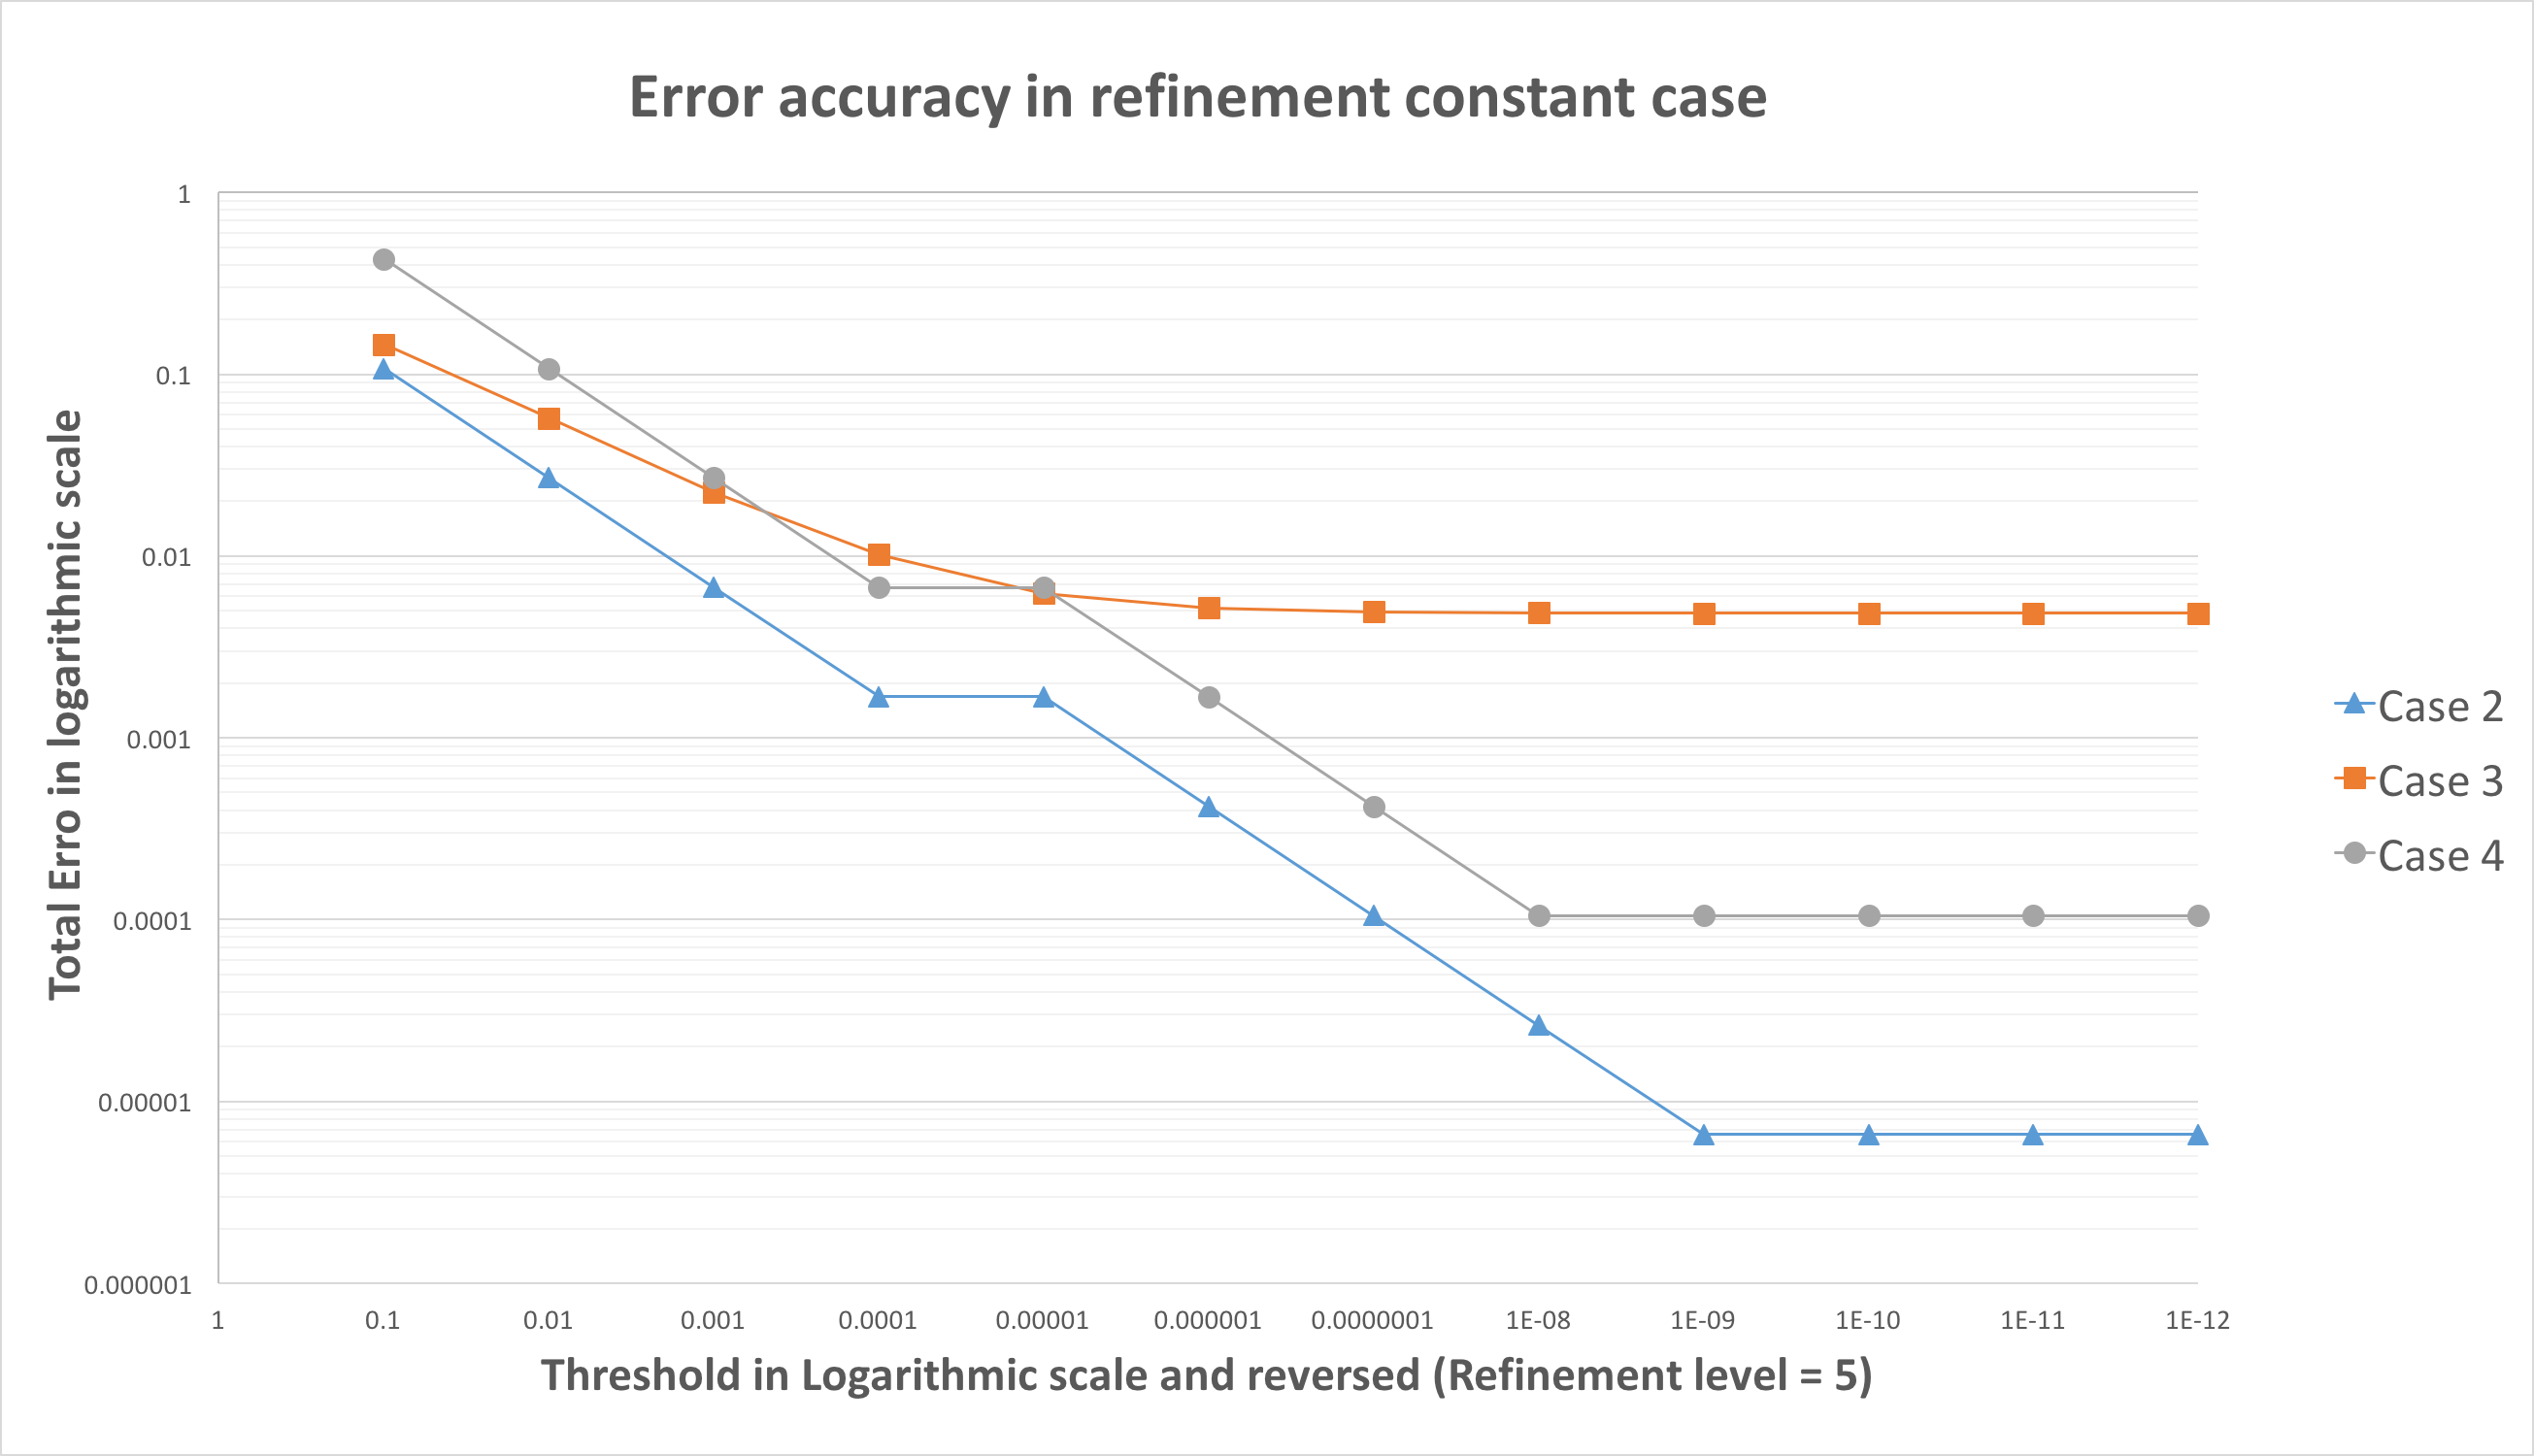
\includegraphics[width =\textwidth]{/results/5/Error-Threshod.png}
		\centering    
	 \caption{Error-Threshold}
       \label{fig:ErrorThreshod}
\end{figure}

As expected, the logarithmic error in both cases decreases with an increase in the level of mesh refinement and becomes constant after one point. It highlights the fact that the mesh independence is achieved in both cases and the results are free from the effect of the mesh refinement. Comparison of figures \ref{fig:ErrorRefinementLevel} and \ref{fig:ErrorThreshod} for case 2 shows much higher error in the threshold-independent approach and a significantly lower error in the refinement-constant approach. The reason is due to the specific definition of the function, in which only a small subsection is relevant for mesh-refinement. As the threshold-independent approach is unable to focus on a specific subsection, the resulting error is higher by a factor of 10 compared to the refinement-constant approach.






		\chapter{Conclusion}
\label{chapter:results}

\section{Conclusion}
This thesis investigated a new adaptive algorithmic approach using sparse grids and combination technique for solving interpolation types of problems. It is advantageous in terms of its robustness less floating point operations(FLOPs). The approach is also suitable for parallelization inherently separation of the problem to independant subproblems. Focused on reaching same order of grid points and memory use as conventional combination methods the approach tries to achieve better accuracy by faster adapting to region with higher order of error by starting from much coarser grid.\\

Several test functions as listed below verify that our implementation works as expected compared to high resolution full grid without adaptation and thus validated  to ensure the functionality under a variety of cases.
\begin{enumerate}
\item $f(x)=x^2+y^2$
\item $f(x)=x^2 \cdot y^2 $
\item $f(x)=\sqrt[2]{x} \cdot \sqrt[2]{y}$
\item $f(x)=16 \cdot x(1-x)y(1-y)$
\end{enumerate}
The default scheme of $\overrightarrow{l}=(4,4)$ for all the nodes of the tree including the root is assumed. In case the test function is not of hyperbolic form with respect to two dimension the bilinear interpolation used in combination technique gives the perfect solution. Simulations are run to observe the error for the local mesh refinement for two independent cases. The error accuracy is observed to be better than full grid mesh refinement. Test cases are also prepared in order to observe the mesh refinement when a predefined error function is enforced to the problem. Besides the predefined error, a simulation based error indicator for local grid has been investigated. The error accuracy is observed to be atleast as effective as the full grid mesh refinement. Under changing levels of refinement in a loop the logarithmic behavior of error as expected form the literature is observed for the solution suggested.\\
To examine the independent effect of the two key factors, threshold for the error and the level of refinement, two approaches are evaluated.
\begin{enumerate}
\item Threshold independent, refinement level changing.
\item Threshold changing, refinement level constant.
\end{enumerate}
The logarithmic error in both cases with an increase of that factor and thus level of refinement becomes saturated after one point since we there is no further refinement. Two different cases are different because one makes the height of the tree to be higher in some local part and the other one ensures that in each level we reach an expected local error. Test case 2 shows much higher error in the threshold-independent approach than the refinement-constant approach due to the definition of the function, in which error in concentrated in one subsection.\\
Overall, the conclusion is that the approach works as expected under different circumstances and while it has been validated for both adaptive and non-adaptive versions it shows the application of this method will be promising for future research and maybe a baseline for prospective scientist. Although It had worked for the cases presented but the author believes certain functions with higher derivatives or with singularities can bring some problems as one first need to detect the errors on the grid position. Therefore, If the variation of the function is inside the blocks basically this method will not work.

\section{Suggestions for future works}
As described earlier the interpolation problem is just a baseline for the adaptive mesh refinement combination technique. However, usually problems which has been tackled extensively in relevant literature e.g. regression and partial differential equation problem require higher complexity. This is becasue the numerical operations there are much more complex as they can be even non-linear in format. Thus definition of error indicator in such problems might be tricky but once we can achieve that we can investigate whether the current method can be applied there. 

		
		
		% ---------------------------------------------------------------------------
		%
		% Appendix
		%
		% ---------------------------------------------------------------------------
		
		\part*{Appendix}
		\addcontentsline{toc}{part}{Appendix}
		
		\appendix %---------------------------------------
		
		\chapter{Appendix}
%\section{Detailed Validation Results}
\label{chapter:DetailedDescriptions}

\section{Source Code}
 \lstset{language=C++}
\begin{lstlisting}[caption= Source code for adaptive combination technique, label=code:combi]
#ifndef COMBINATION_H
#define COMBINATION_H

#include "Fullgrid.h"
#include <stdio.h>

class Combination {
private:
	/*private member variable and function definitions. */

protected:
	/*protected member variable and function definitions. */


public:
	/*public member variable and function definitions. */
	Fullgrid _grid_l1 , _grid_l2 , _grid_lmin;
	Fullgrid _grid_l1_interpolated , _grid_l2_interpolated , _grid_lmin_interpolated;
	Fullgrid _grid_combination;
	int level_max[DIMENSION],level_min[DIMENSION];
	int _Npoints[DIMENSION];

	/** Constructor for the Combination */
	Combination(int* level_1,int* level_2,int* _level_max, int* _level_min, Domain domain)
	:_grid_l1(level_1, domain),_grid_l2(level_2, domain),_grid_lmin(_level_min, domain)
	,_grid_l1_interpolated(_level_max, domain),_grid_l2_interpolated(_level_max, domain)
	,_grid_lmin_interpolated(_level_max, domain),_grid_combination(_level_max, domain){

		for ( int i = 0; i < DIMENSION; ++i ) {
			level_max[i]=_level_max[i];
			level_min[i]=_level_min[i];
		}
		//evaluate case function for each grids needed to be combined
		_grid_l1.evaluate(domain);
		_grid_l2.evaluate(domain);
		_grid_lmin.evaluate(domain);

	}

	/** Destructor Deallocates the data
	 * TASK
	 *  */
	virtual ~Combination() {
		//delete[] ;
	}

	void GetCombination(int* level_1,int* level_2, Domain domain){
		/*apply the method iterate*/
		for ( int i = 0; i < DIMENSION; ++i ) {
			_Npoints[i]=(pow(2,level_max[i]))+1;	//2^l+1
		}
		direct_injection(level_1,_grid_l1,domain,&_grid_l1_interpolated);
		direct_injection(level_2,_grid_l2,domain,&_grid_l2_interpolated);
		direct_injection(level_min,_grid_lmin,domain,&_grid_lmin_interpolated);

		interpolation(level_1,&_grid_l1_interpolated, domain);
		interpolation(level_2,&_grid_l2_interpolated, domain);
		interpolation(level_min,&_grid_lmin_interpolated, domain);

		for ( int i = 0; i < _Npoints[0]; ++i ) {
			for ( int j = 0; j < _Npoints[1]; ++j ) {
				_grid_combination.function_values[i][j]= _grid_l1_interpolated.function_values[i][j] + _grid_l2_interpolated.function_values[i][j] - _grid_lmin_interpolated.function_values[i][j];
			}
		}

	}

	void interpolation(int* level, Fullgrid* interpolated_grid, Domain domain){

		int lower_local_index[DIMENSION], upper_local_index[DIMENSION];
		//interploation in X direction
		for ( int i = 0; i < _Npoints[0]-1; ++i ) {
			for ( int j = 0; j < _Npoints[1]; ++j ) {
				lower_local_index[0]=(int) floor( i/( pow( 2,level_max[0]-level[0] ) ) ) ;
				upper_local_index[0]=lower_local_index[0]+1;
				interpolated_grid->function_values[i][j]= ((double) ( upper_local_index[0] * ( pow( 2,level_max[0]-level[0] ) ) - i))/((double) ( pow( 2,level_max[0]-level[0] ) )) * interpolated_grid->function_values[(int) (lower_local_index[0]* pow( 2,level_max[0]-level[0] ) )][j]+ ((double) ( i - lower_local_index[0] * ( pow( 2,level_max[0]-level[0] ) ) ))/((double) ( pow( 2,level_max[0]-level[0] ) )) * interpolated_grid->function_values[(int) (upper_local_index[0]*pow( 2,level_max[0]-level[0] ))][j];
			}
		}
		//interploation in Y direction
		for ( int i = 0; i < _Npoints[0]; ++i ) {
			for ( int j = 0; j < _Npoints[1]-1; ++j ) {
				lower_local_index[1]=(int) floor( j/( pow( 2,level_max[1]-level[1] ) ) );
				upper_local_index[1]=lower_local_index[1]+1;
				interpolated_grid->function_values[i][j]= ((double) ( upper_local_index[1] * ( pow( 2,level_max[1]-level[1] ) ) - j))/((double) ( pow( 2,level_max[1]-level[1] ) )) * interpolated_grid->function_values[i][(int) (lower_local_index[1]*pow( 2,level_max[1]-level[1] ))]+ ((double) ( j - lower_local_index[1] * ( pow( 2,level_max[1]-level[1] ) ) ))/((double) ( pow( 2,level_max[1]-level[1] ) )) * interpolated_grid->function_values[i][(int) (upper_local_index[1]*pow( 2,level_max[1]-level[1] ))];
			}
		}

	}

	void direct_injection(int* level, Fullgrid _grid, Domain domain, Fullgrid* _projected_grid){

		// Initialize to zero
		for ( int i = 0; i < _Npoints[0]; ++i ) {
			for ( int j = 0; j < _Npoints[1]; ++j ) {
				_projected_grid->function_values[i][j]= 0;
			}
		}

		//for all local values we directly project to global
		int _Npoints_local[DIMENSION];
		for ( int i = 0; i < DIMENSION; ++i ) {
			_Npoints_local[i]=(pow(2,level[i]))+1;	//2^l+1
		}

		for ( int i = 0; i < _Npoints_local[0]; ++i ) {
			for ( int j = 0; j < _Npoints_local[1]; ++j ) {
				_projected_grid->function_values[ (int) (i*pow( 2,level_max[0]-level[0] ))][ (int) (j*pow( 2,level_max[1]-level[1] )) ]= _grid.function_values[i][j];
			}
		}
	}

};

#endif
\end{lstlisting}

 \lstset{language=C++}
\begin{lstlisting}[caption= Source code for Full grid method, label=code:fullG]
#ifndef FULLGRID_H
#define FULLGRID_H

#include "Definitions.h"
/*here Full grid structure will be build*/

class Fullgrid {
public:
	/*public member variable and function definitions. */
	int _Npoints[DIMENSION];
	double _mesh_size[DIMENSION];
	double** function_values;
	double *position_d1, *position_d2;

	/** Default constructor for the fullgrid
	 */
	Fullgrid(int* level, Domain _domain) {
		for ( int i = 0; i < DIMENSION; ++i ) {
			_Npoints[i]=(pow(2,level[i]))+1;	//2^l+1
			_mesh_size[i]= (_domain.end_point[i] - _domain.start_point[i]) / (pow(2,level[i]) );	//2^-l
		}
		position_d1 = new double[ _Npoints[0] ];
		position_d2 = new double[ _Npoints[1] ];
		//Assign first dimension
		function_values = new double*[_Npoints[0]];
		//Assign second dimension
		for(int i = 0; i <_Npoints[0] ; i++){
			function_values[i] = new double[_Npoints[1]];
		}
	}

	//copy constructor
	Fullgrid(const Fullgrid& _copyfromfullgrid) {
		for ( int i = 0; i < DIMENSION; ++i ) {
			_Npoints[i]=_copyfromfullgrid._Npoints[i];	//2^l+1
			_mesh_size[i]= _copyfromfullgrid._mesh_size[i];
		}
		position_d1 = new double[ _Npoints[0] ];
		position_d2 = new double[ _Npoints[1] ];
		function_values = new double*[_Npoints[0]];
		for(int i = 0; i <_Npoints[0] ; i++){
			function_values[i] = new double[_Npoints[1]];
		}
		for ( int j_1 = 0; j_1 < _Npoints[0]; ++j_1 ) {
			position_d1[j_1]=_copyfromfullgrid.position_d1[j_1];
		}
		for ( int j_2 = 0; j_2 < _Npoints[1]; ++j_2 ) {
			position_d2[j_2]=_copyfromfullgrid.position_d2[j_2];
		}
		//		**(_array) = new double[index_size_global]();  ///Zero-initialize (somehow doesn't work here)
		for ( int i = 0; i < _Npoints[0]; ++i ) {
			for ( int j = 0; j < _Npoints[1]; ++j ) {
				function_values[i][j]= _copyfromfullgrid.function_values[i][j];  //X^2*Y^2 - TASK (implement new function to do here)
			}
		}

	}

	//Assignment operator
	Fullgrid& operator=(const Fullgrid& _equalfullgrid){
		if (this!=&_equalfullgrid){
			for ( int i = 0; i < DIMENSION; ++i ) {
				_Npoints[i]=_equalfullgrid._Npoints[i];	//2^l+1
				_mesh_size[i]= _equalfullgrid._mesh_size[i];
			}
			position_d1 = new double[ _Npoints[0] ];
			position_d2 = new double[ _Npoints[1] ];
			function_values = new double*[_Npoints[0]];
			//Assign second dimension
			for(int i = 0; i <_Npoints[0] ; i++){
				function_values[i] = new double[_Npoints[1]];
			}

			for ( int j_1 = 0; j_1 < _Npoints[0]; ++j_1 ) {
				position_d1[j_1]=_equalfullgrid.position_d1[j_1];
			}
			for ( int j_2 = 0; j_2 < _Npoints[1]; ++j_2 ) {
				position_d2[j_2]=_equalfullgrid.position_d2[j_2];
			}
			//		**(_array) = new double[index_size_global]();  ///Zero-initialize (somehow doesn't work here)
			for ( int i = 0; i < _Npoints[0]; ++i ) {
				for ( int j = 0; j < _Npoints[1]; ++j ) {
					function_values[i][j]= _equalfullgrid.function_values[i][j];  //X^2*Y^2 - TASK (implement new function to do here)
				}
			}
		}
		return *this;
	}

	/** Destructor Deallocates the data
	 * TASK
	 */
	virtual ~Fullgrid() {
		delete[] function_values;
		delete[] position_d1;
		delete[] position_d2;
	}

	/*evaluates function value for TestFunction defined in definitions*/
	void evaluate(Domain _domain){

		for ( int j_1 = 0; j_1 < _Npoints[0]; ++j_1 ) {
			position_d1[j_1]=_domain.start_point[0]+j_1*_mesh_size[0];
		}
		for ( int j_2 = 0; j_2 < _Npoints[1]; ++j_2 ) {
			position_d2[j_2]=_domain.start_point[1]+j_2*_mesh_size[1];
		}
		//		**(_array) = new double[index_size_global]();  ///Zero-initialize (somehow doesn't work here)
		for ( int i = 0; i < _Npoints[0]; ++i ) {
			for ( int j = 0; j < _Npoints[1]; ++j ) {
				function_values[i][j]= TestFunction(position_d1[i],position_d2[j]);  //X^2*Y^2 - TASK (implement new function to do here)
			}
		}
	}



	/** notice: by introducing domain it may need to change accordingly by adding level of domain
	by putting level_max it will give the index for full grid
	 */
	/** here a multidimensional indices which is stored in 1D array called "index" is mapped to a value to use in grid
	 *  TASK
	 */
	/**
	int Map2arrayIndex_local(int * index, int*level)  {
		int multiplier=1,mapped_index=0;
		for loop over dimensions to get to index
		for ( int i = 0; i < DIMENSION; ++i ) {
			_Npoints[i]=(pow(2,level[i]))+1;	//2^l+1
			if (i>0){
				multiplier*=_Npoints[i-1];
			}
			mapped_index+=index[i]*multiplier;
		}
		return mapped_index;
	}
	 */
private:

};

#endif

\end{lstlisting}

 \lstset{language=C++}
\begin{lstlisting}[caption= Source code for quad trees, label=code:quad]
#ifndef QUADTREE_H
#define QUADTREE_H

#include "Definitions.h"
#include "Combination.h"
#include "Visual.h"
#include <math.h>

class Node{
public:
	bool refined_factor; //whether the node should be refined or not 0=no refinement 1=to be refined
	double total_error_in_node; //total error calculated in the subtree
	double total_error_in_node_using_predefined_function; //
	int node_level;
	string name;
	Domain domain;


	Fullgrid* beforecombi_fullgrid;
	Fullgrid* aftercombi_fullgrid;
	Fullgrid* difference_grid;

	Node* parent_node;
	Node* NW_child_node;
	Node* NE_child_node;
	Node* SE_child_node;
	Node* SW_child_node;


	//constructor
	Node(): parent_node(NULL),NW_child_node(NULL),NE_child_node(NULL),SE_child_node(NULL),SW_child_node(NULL){};

};


#endif
\end{lstlisting}

 \lstset{language=C++}
\begin{lstlisting}[caption= Source code for solution, label=code:sol]
#ifndef SOLUTION_H
#define SOLUTION_H

#include "QuadTree.h"
#include "Definitions.h"
#include "Combination.h"
#include "Visual.h"
#include <math.h>
#include <iostream>
using namespace std;

#include <sys/types.h>
#include <sys/stat.h>
#include <unistd.h>

bool solve(Node* current_node);

void expand_Quad(Node* current_node);

double evaluate_predefinedError(Domain new_domain);

void AdaptiveRefinement(Node* current_node);

bool solve(Node* current_node){

	current_node->beforecombi_fullgrid	= new Fullgrid(level_max, current_node->domain);
	current_node->aftercombi_fullgrid	= new Fullgrid(level_max, current_node->domain);
	current_node->difference_grid		= new Fullgrid(level_max, current_node->domain);

	current_node->beforecombi_fullgrid->evaluate(current_node->domain);

	Combination* _combinationSolution= new Combination(level_1,level_2,level_max,level_min,current_node->domain);
	_combinationSolution->GetCombination(level_1,level_2, current_node->domain);
	current_node->aftercombi_fullgrid=&_combinationSolution->_grid_combination;

	//**************************Calculation of difference value between sparse grid combination and normal full grid and computing total error of the node
	current_node->total_error_in_node=0;
	for ( int i = 0; i < _Npoints[0]; ++i ) {
		for ( int j = 0; j < _Npoints[1]; ++j ) {
			current_node->difference_grid->function_values[i][j]= current_node->beforecombi_fullgrid->function_values[i][j] - current_node->aftercombi_fullgrid->function_values[i][j];
			if (current_node->difference_grid->function_values[i][j]<0){
				current_node->total_error_in_node-=current_node->difference_grid->function_values[i][j];//if it's negative then make it positive and add (sum + absolute(x)) = sum - x
			}
			else{
				current_node->total_error_in_node+=current_node->difference_grid->function_values[i][j];//if it's positive then just add (sum + absolute(x)) = sum + x
			}

		}
	}
	//**************************
	if (USE_PREDEFINED_ERROR==0){ //if we use predefined then we don't use the error calculated
		if (current_node->total_error_in_node>TRESHOLD_ERROR && current_node->node_level<MAX_ADAPTATION_LEVEL){   //if error is not satisfied or we didn't go too far then make a new refinement
			current_node->refined_factor=1;
		}
		else {
			current_node->refined_factor=0;
		}
	}
	else if (USE_PREDEFINED_ERROR==1){
		current_node->total_error_in_node_using_predefined_function = evaluate_predefinedError(current_node->domain);
		if (current_node->total_error_in_node_using_predefined_function>TRESHOLD_ERROR && current_node->node_level<MAX_ADAPTATION_LEVEL){   //if error is not satisfied or we didn't go too far then make a new refinement
			current_node->refined_factor=1;
		}
		else {
			current_node->refined_factor=0;
		}
	}


	//if only we need refining then we draw that branch


	if (current_node->refined_factor==0){
		if (WRITE_VTK==1){
			struct stat st_results = {0};
			if (stat("Results", &st_results) == -1) {
				mkdir("Results", 0700);
			}
			//vtk with subdirectory for no combination
			struct stat st_nocombi = {0};
			if (stat("Results/no_combination", &st_nocombi) == -1) {
				mkdir("Results/no_combination", 0700);
			}
			string fullgrid_name="./Results/no_combination/noCombi"  + std::to_string(current_node->node_level) +  current_node->name;
			const char *cfullgrid_name = fullgrid_name.c_str();
			write_vtkFile(cfullgrid_name,current_node->domain,current_node->beforecombi_fullgrid);
			//vtk with subdirectory for combination
			struct stat st_combi = {0};
			if (stat("Results/combination", &st_combi) == -1) {
				mkdir("Results/combination", 0700);
			}
			string combigrid_name="./Results/combination/Combi"  + std::to_string(current_node->node_level) +  current_node->name;
			const char *ccombigrid_name = combigrid_name.c_str();
			write_vtkFile(ccombigrid_name,current_node->domain,current_node->aftercombi_fullgrid);
			//vtk with subdirectory for no combination
			struct stat st_diff = {0};
			if (stat("Results/difference_grid", &st_diff) == -1) {
				mkdir("Results/difference_grid", 0700);
			}
			string diffgrid_name="./Results/difference_grid/difference" + std::to_string(current_node->node_level) + current_node->name;
			const char *cdiffgrid_name = diffgrid_name.c_str();
			write_vtkFile(cdiffgrid_name,current_node->domain,current_node->difference_grid);
		}
	}

	return current_node->refined_factor;
}

void expand_Quad(Node* current_node){

	//making this node parent of all children
	current_node->SW_child_node = new Node();
	current_node->SE_child_node = new Node();
	current_node->NW_child_node = new Node();
	current_node->NE_child_node = new Node();
	current_node->SW_child_node->parent_node=current_node;
	current_node->SE_child_node->parent_node=current_node;
	current_node->NW_child_node->parent_node=current_node;
	current_node->NE_child_node->parent_node=current_node;
	//naming scheme
	current_node->SW_child_node->name=current_node->name+"SW";
	current_node->SE_child_node->name=current_node->name+"SE";
	current_node->NW_child_node->name=current_node->name+"NW";
	current_node->NE_child_node->name=current_node->name+"NE";
	//Node level is added one time
	current_node->SW_child_node->node_level=current_node->node_level+1;
	current_node->SE_child_node->node_level=current_node->node_level+1;
	current_node->NW_child_node->node_level=current_node->node_level+1;
	current_node->NE_child_node->node_level=current_node->node_level+1;
	//Setting new domains for all four children
	//South West child
	current_node->SW_child_node->domain.start_point[0] = current_node->domain.start_point[0];
	current_node->SW_child_node->domain.start_point[1] = current_node->domain.start_point[1];
	current_node->SW_child_node->domain.end_point[0]   = (current_node->domain.start_point[0]+current_node->domain.end_point[0])/2;
	current_node->SW_child_node->domain.end_point[1]   = (current_node->domain.start_point[1]+current_node->domain.end_point[1])/2;
	//South East child
	current_node->SE_child_node->domain.start_point[0] = (current_node->domain.start_point[0]+current_node->domain.end_point[0])/2;
	current_node->SE_child_node->domain.start_point[1] = current_node->domain.start_point[1];
	current_node->SE_child_node->domain.end_point[0]   = current_node->domain.end_point[0];
	current_node->SE_child_node->domain.end_point[1]   = (current_node->domain.start_point[1]+current_node->domain.end_point[1])/2;
	//North West Child
	current_node->NW_child_node->domain.start_point[0] = current_node->domain.start_point[0];
	current_node->NW_child_node->domain.start_point[1] = (current_node->domain.start_point[1]+current_node->domain.end_point[1])/2;
	current_node->NW_child_node->domain.end_point[0]   = (current_node->domain.start_point[0]+current_node->domain.end_point[0])/2;
	current_node->NW_child_node->domain.end_point[1]   = current_node->domain.end_point[1];
	//North East Child
	current_node->NE_child_node->domain.start_point[0] = (current_node->domain.start_point[0]+current_node->domain.end_point[0])/2;
	current_node->NE_child_node->domain.start_point[1] = (current_node->domain.start_point[1]+current_node->domain.end_point[1])/2;
	current_node->NE_child_node->domain.end_point[0]   = current_node->domain.end_point[0];
	current_node->NE_child_node->domain.end_point[1]   = current_node->domain.end_point[1];
}

double evaluate_predefinedError(Domain new_domain){
	double _error=0;
	//calculation of positions might be for no reason after evaluate function has been called once
	int Ncell[DIMENSION];
	double mesh_size_domain[DIMENSION];
	double *cellposition_d1, *cellposition_d2;

	for ( int i = 0; i < DIMENSION; ++i ) {
		Ncell[i]=(pow(2,level_max[i]));	//2^l cell
		mesh_size_domain[i]= (new_domain.end_point[i] - new_domain.start_point[i]) / (pow(2,level_max[i]) );	//2^-l
	}
	cellposition_d1 = new double[ Ncell[0] ];
	cellposition_d2 = new double[ Ncell[1] ];

	for ( int j_1 = 0; j_1 < Ncell[0]; ++j_1 ) {
		cellposition_d1[j_1]=new_domain.start_point[0]+j_1*mesh_size_domain[0]+mesh_size_domain[0]/2.0;
	}
	for ( int j_2 = 0; j_2 < Ncell[1]; ++j_2 ) {
		cellposition_d2[j_2]=new_domain.start_point[1]+j_2*mesh_size_domain[1]+mesh_size_domain[1]/2.0;
	}
	for ( int i = 0; i < _Npoints[0]; ++i ) {
		for ( int j = 0; j < _Npoints[1]; ++j ) {
			_error+= ErrorFunction(cellposition_d1[i],cellposition_d2[j]);  //X^2*Y^2 - TASK (implement new function to do here)
		}
	}
	return _error;
}

void AdaptiveRefinement(Node* current_node){

	current_node->refined_factor=solve(current_node);

	if (current_node->refined_factor==1)
	{
		expand_Quad(current_node);

		AdaptiveRefinement(current_node->SW_child_node);
		AdaptiveRefinement(current_node->SE_child_node);
		AdaptiveRefinement(current_node->NW_child_node);
		AdaptiveRefinement(current_node->NE_child_node);
	}

}

double compute_error(Node* current_node){
	static int j=0;

	double current_error=0;
	if (current_node->refined_factor==0){
		current_error+=current_node->total_error_in_node;
		j++;
		//cout<<"current one we are at j= "<< j <<" with name= "<<current_node->name<<endl;
		//cout<<"total error in node was=" << current_node->total_error_in_node<<endl;
		const char *temp = current_node->name.c_str();
		if (USE_PREDEFINED_ERROR==1){printf ("total error predefined for %s =  %f\n",temp,current_node->total_error_in_node_using_predefined_function);	}

	}
	else if (current_node->refined_factor==1)
	{
		current_error+=compute_error(current_node->SW_child_node);
		current_error+=compute_error(current_node->SE_child_node);
		current_error+=compute_error(current_node->NW_child_node);
		current_error+=compute_error(current_node->NE_child_node);
	}

	return current_error;
}

#endif

\end{lstlisting}


		
		%Activate if you want to show all the references
		%*\nocite{*}
	


  \clearemptydoublepage
  \bibliography{bibliography/literature}
	
	
	
 
\end{document}

